% Chapter 3
\chapter{Muon Identification in the \lhcb High Level Trigger}
\label{Muon_id_hlt}

The \lhcb trigger system has been briefly described in \secref{lhcb_trigger}. The current chapter focuses on the muon identification
part of the trigger. Muons are important for the \lhcb experment, since a large fraction of its physics programme is based on
the identification of muons in the final state: for example the measurement of \phis through \BsJpsiPhi decays, the study of CP
violation through semileptonic decays, and the measurement
in several rare decays such as \BdKstmumu and \Bsmm. It is therefore of major importance to maintain and improve the efficiency
and purity of identified muons in the Run II data-taking of LHCb. During the shutdown period between \runone and II, effort has
been put to re-optimize the software performing the muon identification. A unified software that can be run both online in the
LHCb software trigger and in the offline reconstruction has been obtained. Furthermore, the detection effciency of low momentum
muons is improved given the available comptuting resources of \runtwo. Low momentum muons are intreasting {\color{red} for these analysis, site diego kaon physics}
A brief description of the unified \muonID code is given in \secref{muid_hlt1}. The low momentum muon efficiency optimization
is addressed in \secref{mvm_algorrithm}.

\section{\muonID in \hlt}
\label{muid_hlt1}

The \muonID \cite{LHCb-PUB-2009-013,LHCb-PUB-2010-002} that is used both in the High Level Trigger (\hlt) \cite{LHCb-PUB-2011-017}
and in the offline event processing has been revisited in view of the \lhc \runtwo.
Note that during \runone the \hlt version of the \muonID software was different from the one used offline in order
to comfront with the available computing resources. The main reasons for revisiting the software are;
First to unify the \muonID used in \hlt and offline as much as possible.
Second to optimize the trigger efficiency of low transverse momentum muons.
In particular, the \muonID has undergone a significant refactory resulting in a modularised common code base
between \hlt and offline event processing \cite{kevinThesis}. Bacause of that
muon indentification in the \hltone and offline are identical \footnote{The \muonID in \hlttwo was the same as offline already in \runone.},
which combined with the novel {\it online detector alignment and calibration} endeavour \cite{Aaij:2016rxn,LHCb-PROC-2015-024},  allows for the trigger
to produce offline quality data. After the modularization readability and maintenance of the code were improved.
An increase in performance of the \muonID code was also achieved both in CPU and memory usage.

The algorithm sequence of the \hltone muon trigger lines\footnote{The term trigger line is defined in \secref{det_trigger}}
during \runone was tuned in order to comply with the output rate limitations given the existinng computing infrastructure,
named {\it Event Filter Farm} (EFF). Since then the EFF has undergone a significant upgrade resulting in an
increased processing power along with increased storage capabilities. In view of this infrastructure upgrade
as well as the \runtwo \lhc running conditions the total output rate of the entire trigger system was increased
from 5\khz to 12.5\khz, see \figref{det_trigger_scheams}. The impact on the \hltone is that its output rate is
roughly doubled and additional processing time is available. This boost in computing power allowed for changes
in the \muonID alogorithm sequence regarding muons above 500 \mevc. Particularly the \mvm algorithm that filtered
the above tracks during \runone, see \figref{hlt1_algo_seq}, was removed.
Instead all these muons are passed directly to the next stages of the \muonID software.

\subsection{\hltone muon lines algorithm sequence}
\label{hlt1run2}

The role of the trigger system and the decitions that it provides were presented in \secref{det_trigger},
where the concept of a trigger line is also introduced in the previous section. The \hltone muon trigger lines are
mainly organized in single muon and dimuon ones; both exploit the same muon identification procedure which
is described in the current subsection. The efficiency of the muon lines during \runone is shown in \figref{det_run_one_muon_line_eff}.
It can be observed that a low \pt turn on and a large efficiency loss in the dimuon lines are present.
In order to understand the origin of this efficiency loss the \hltone algorithm sequence is analysed further.
The \hltone muon trigger lines sequence during \runone is shown in the left of \figref{hlt1_algo_seq}.
A brief summary of this procedure is given in the current subsection, for a full description see \cite{LHCb-PUB-2011-017}.

During \runone the muon identification started directly from \veloTracks\footnote{see \figref{track_types}}
and filtered out keeping good muon candidates before running any tracking algotrithm\footnote{see \secref{det_tracking}}.
This is done by the \mvm algorithm, see \secref{sec:muon_matching} and \cite{LHCb-PUB-2011-017} for the full discription.
Subsequently the \FwD algorithm uses information from the tracking stations and upgrades the \veloTracks to long tracks, defined in \secref{det_tracking}.
After this, the \isMuon algorithm is applied\footnote{\isMuon is an alias for the \muonID software.}.
In addition there are some quality cuts between each algorithm step, such as the number of hits produced in the
\velo sub-detector by a track or the fitted track $\chisq/\nDoF$ as well as momentum cuts applied after the \FwD
tracking algorithm. The minimum momentum and transverse momentum was 6 \gevc and 0.5 \gevc respectively.

\begin{figure}[t]
  \centering
  \tikzsetnextfilename{hlt1_alg_seq_old}
  \scalebox{1}{\begin{tikzpicture}[node distance=.5cm and 2.cm]
       \node [block, source] (test-0) {\veloTracks};
       \node [block, op, below=of test-0, ] (test-1) {\mvm};
        \node [block, op,  below=of test-1] (test-2) {\FwD};
        \node [block, op, below=of test-2] (test-3) {\isMuon};
        \node [block, op, below=of test-3] (test-4) {\fitTrack};
        \node [block, op, below=of test-4] (test-5) {\diMuons };
        \node [block, cut, below=of test-5] (test-6) {Additional cuts};
        \node [block, sink, below=of test-6] (test-7) {Decision};
       \path [line] (test-0) -- (test-1);
       \path [line] (test-1) -- (test-2);
       \path [line] (test-2) -- (test-3);
       \path [line] (test-3) -- (test-4);
       \path [line] (test-4) -- (test-5);
       \path [line] (test-5) -- (test-6);
       \path [line] (test-6) -- (test-7);
\end{tikzpicture}
}
  \tikzsetnextfilename{hlt1_alg_seq_new}
  \scalebox{1}{\begin{tikzpicture}[node distance=.5cm and 2.cm, every node/.style={rectangle,fill=white}]
       \node [block, source] (test-0) {Velo Tracks};
       \node [block, cut, below=of test-0, ] (test-1) {$\pt > 500$ MeV/c};
       \node [block, op, below=of test-1,  xshift=2cm] (test-2) {MatchVeloTTMuon};
       \node [block, op, below=of test-2] (test-20) {Forward Tracking};
       \node [block, op, below=of test-20] (test-4) {Fit track};
        \node [block, source, below=of test-1,  xshift=-2cm] (test-3) {Get long track};
        \node [block, cut, below=of test-4,   xshift=-2cm] (test-5) {Cuts on track};
        \node [block, op, below=of test-5] (test-6) {IsMuon};
        \node [block, op, below=of test-6] (test-7) {Make dimuons };
	\node [block, cut, below=of test-7] (test-8) {Additional cuts};
	\node [block, sink,below=of test-8] (test-9) {Decision};
       \path [line] (test-0) -- (test-1);
       \path [line] (test-1) -- node {no} (test-2);
       \path [line] (test-1) -- node {yes} (test-3);
       \path [line] (test-2) -- (test-20);
       \path [line] (test-20) -- (test-4);
       \path [line] (test-3) -- (test-5);
       \path [line] (test-4) -- (test-5);
       \path [line] (test-5) -- (test-6);
       \path [line] (test-6) -- (test-7);
       \path [line] (test-7) -- (test-8);
       \path [line] (test-8) -- (test-9);
\end{tikzpicture}
}
 \caption{ \runone and \runtwo \hltone algoriths compared. }
  \label{hlt1_algo_seq}
\end{figure}

A detailed efficiency breakdown \cite{kevinThesis} of the \runone \hltone muon lines showed that the main source of efficiency
loss is due to the quality and momentum cuts. Also the \mvm algorithm is reduces the efficiency by roughly $4\%$.
The updated code sequence of the \hltone muon lines is documented in \cite{kevinThesis}.
% Whilst the upgrade of the \mvm algorithm for softer muons in \secref{sec:matchvelottmuon}.

In the the \runtwo updated \hltone algorithm sequence of \figref{det_run_two_trigger}.
For the majority of the tracks, which have transverse momentum larger than 500 MeV, the sequence is different with respect to
Run I: full tracking is performed for these tracks, so that the start for muon finding is already with long tracks.
After soft quality cuts these get passed through the standard \isMuon algorithm in order to be identified;
positively identified muons are then combined into dimuons as in Run I.
The combination of the use of long tracks and standard muon identification is much more efficient than the
procedure in Run I, and is exactly the same as the one of offline reconstruction.
Tracks with transverse momentum smaller than 500 MeV cannot be immediately upgraded to long tracks for timing reasons.
However some of them will be muons, and the efficiency for these could be recovered using a different strategy,
explained in \secref{mvm_algorrithm}.


\section{MatchVeloMuon update}
\label{mvm_algorrithm}
In \runone all \veloTracks in \hltone were filtered by the \mvm algorithm, as mentioned in \secref{hlt1run2}.
Given the available information from the muon stations, the latter algorithm performs a quick check on whether a
\velo track is compatible with being identified as a muon by the subsequent tracking algorithms, before these
algorithms are actually run. If the \velo track passes certain simple requirements it
is accepted, otherwise it is discarded permanently and not processed further by the \hlt muon lines. As a result
valuable computing time is saved, since the \FwD tracking and fitting algorithms are time costly.

\subsection{The MatchVeloMuon algorithm}
\label{sec:muon_matching}

The \mvm algorithm takes a \velo track as input and checks whether it is compatible with being a muon by
searching for hits inside an area in the M3 muon station. This area is called {\it Field of Interest} (FoI).
The hits found inside the M3 FoI are called {\it seed hits} and they are used as starting space points to look
for more hits in the rest of the muon stations. For each M3 seed hit, additional hits are searched for
by extrapolating from each M3 seed hit further to the rest of the muon stations.
Since there is no magnetic field between the muon stations, the above-mentioned extrapolations are simple straight lines.
The corresponding FoIs for the rest of the muon stations are smaller, compared to the M3 FoI, since there
is no additional deflection involved. These smaller FoIs do account for the fact that the presence of heavy material
between the muon stations affects the trajectory of a muon passing through. This effect is called {\it multiple
scattering}, and it is more pronounced for low momentum tracks.

M3 is the first station to search for hits that could be assigned to a certain \velo track: This is because the
number of hits in M2 is large compared to M3, see Figure 3.2 in \cite{roelThesis}; Thus an initial \velo track
candidate would result in a large number of seed hits, which is not computationally feasible. Note that the muon
reconstruction algorithm (\isMuon) starts from the M3 station as well, for the same reason.

Regarding the issue of FoI size computation: As it can be seen in \figref{lhcb_detector_cross_section},
the \lhcb magnet is between the \velo tracker and the muon system. Thus a track traversing the area from the
\velo to the muon stations is deflected by the magnetic field based on its momentum.  The lower the momentum
of a track the more it is deflected by the magnetic field. No momentum or charge information is available for
the \velo track before the \FwD algorithm is run. Thus, the size of the M3 FoI is defined assuming a minimum
track momentum of 6 \gevc. This particular momentum value corresponds to the threshold value of the subsequent
\isMuon algorithm.

At least three hits in the muon stations M2-M5 are required by the \mvm algorithm in order to accept the initial \velo track.
At the end of this procedure all {\it muon candidate tracks} that could result from an initial \velo track are considered.
Within the scope of the current chapter a muon candidate is defined as the track formed by muon hits only.
Note that at this stage of the algorithm an estimate of the momentum of the initial \velo track becomes available
for each candidate muon track using the kick method \cite{Hommels:999327}. The kick method provides an estimate
of the track momentum by comparing the slope of the track before and after passing through the \lhcb magnetic
field. The relation between the change in slope and the track momentum is empirically estimated in \cite{roelThesis}.

As a last step the candidate muon tracks originating from the above procedure are filtered by a $\chisq/\nDoF$
requirement. The \chisq is simple to compute since there is no magnetic field in the region of the muon stations
and all tracks are almost straight lines. Deviations from the straight line approach are only due to
multiple scattering, mentioned above. The \chisq requirement reduces the chances that random combinations of muon hits
can fake a muon track. The requirement is particularly useful for low momentum tracks for which the number
of M3 seed hits is larger. This is because the corresponding M3 FoI are larger, and thus the number of possible
random combinations of muon tracks increases.

An important detail that increases the discriminating power of the above-mentioned \chisq is based on the
assumption that the bending induced by the \lhcb magnetic field can be approximated by a single instantaneous
change in the slope of the charged particle trajectory. This instantaneous change happens at the so called
{\it focal plane}. The special coordinates of the focal plane form a {\it magnet hit}, which is included in
the \chisq computation, as if it was an actual hit. Note that this instantaneous change in slope is an approximation
and in reality the track follows a smooth trajectory inside the whole area of the magnetic field, see \figref{det_evt_display}.
However estimating this trajectory consumes valuable computation time during \hltone run-time, while \mvm can perform
efficiently enough without a smooth track trajectory using the focal
pane approximation. The position of the $z$ focal plane as a function of the track parameters has been studied
\cite{Hommels:999327} and is used in the \mvm algorithm. As mentioned in the beginning of the paragraph including
information on the estimated focal plane helps rejecting fake muon tracks.
This is because the magnet hit essentially requires that the muon hits are aligned in a straight line that
also passes from the magnet hit. The latter is true for real muon tracks only.

\subsection{Upgrade to MatchVeloTTMuon}
\label{sec:matchvelottmuon}
As mentioned in \secref{muid_hlt1}, due to the increased \hltone rate in \runtwo it becomes possible to
remove the \mvm algorithm from the sequence of the \hltone muon lines and instead push all \veloTracks with
$\pt>500 \mevc$ further in the algorithm sequence. Additionally, another improvement is the use of
information from the \ttracker tracker when reconstructing \veloTracks \cite{LHCb-PUB-2015-005}.
Note that the \ttracker is positioned close enough to the \lhcb magnet to allow for an initial track momentum estimate.
The \ttracker momentum resolution is inferior, $\sim 15\%$, compared to the one of a Long track.
However, adding information from the \ttracker the purity of the of the \veloTracks increases \cite{Bowen:2105078}.
This is achieved by reducing the number of fake tracks also known as {\it ghost tracks}.
The resulting set of tracks is called \veloTTracks.

The above-mentioned improvements offer opportunities for reconstructing muons with $\pt<500 \mevc$,
hereafter low momentum muons, by improving the old \mvm algorithm and using it in newly introduced
\hltone muon lines which aim at reconstructing low \pt muons.

\begin{figure}[t]
  \centering
    \tikzsetnextfilename{pt_zoom_efficiencies}
    \scalebox{.6}{\begin{tikzpicture}
\pgfdeclareplotmark{cross} {
\pgfpathmoveto{\pgfpoint{-0.3\pgfplotmarksize}{\pgfplotmarksize}}
\pgfpathlineto{\pgfpoint{+0.3\pgfplotmarksize}{\pgfplotmarksize}}
\pgfpathlineto{\pgfpoint{+0.3\pgfplotmarksize}{0.3\pgfplotmarksize}}
\pgfpathlineto{\pgfpoint{+1\pgfplotmarksize}{0.3\pgfplotmarksize}}
\pgfpathlineto{\pgfpoint{+1\pgfplotmarksize}{-0.3\pgfplotmarksize}}
\pgfpathlineto{\pgfpoint{+0.3\pgfplotmarksize}{-0.3\pgfplotmarksize}}
\pgfpathlineto{\pgfpoint{+0.3\pgfplotmarksize}{-1.\pgfplotmarksize}}
\pgfpathlineto{\pgfpoint{-0.3\pgfplotmarksize}{-1.\pgfplotmarksize}}
\pgfpathlineto{\pgfpoint{-0.3\pgfplotmarksize}{-0.3\pgfplotmarksize}}
\pgfpathlineto{\pgfpoint{-1.\pgfplotmarksize}{-0.3\pgfplotmarksize}}
\pgfpathlineto{\pgfpoint{-1.\pgfplotmarksize}{0.3\pgfplotmarksize}}
\pgfpathlineto{\pgfpoint{-0.3\pgfplotmarksize}{0.3\pgfplotmarksize}}
\pgfpathclose
\pgfusepathqstroke
}
\pgfdeclareplotmark{cross*} {
\pgfpathmoveto{\pgfpoint{-0.3\pgfplotmarksize}{\pgfplotmarksize}}
\pgfpathlineto{\pgfpoint{+0.3\pgfplotmarksize}{\pgfplotmarksize}}
\pgfpathlineto{\pgfpoint{+0.3\pgfplotmarksize}{0.3\pgfplotmarksize}}
\pgfpathlineto{\pgfpoint{+1\pgfplotmarksize}{0.3\pgfplotmarksize}}
\pgfpathlineto{\pgfpoint{+1\pgfplotmarksize}{-0.3\pgfplotmarksize}}
\pgfpathlineto{\pgfpoint{+0.3\pgfplotmarksize}{-0.3\pgfplotmarksize}}
\pgfpathlineto{\pgfpoint{+0.3\pgfplotmarksize}{-1.\pgfplotmarksize}}
\pgfpathlineto{\pgfpoint{-0.3\pgfplotmarksize}{-1.\pgfplotmarksize}}
\pgfpathlineto{\pgfpoint{-0.3\pgfplotmarksize}{-0.3\pgfplotmarksize}}
\pgfpathlineto{\pgfpoint{-1.\pgfplotmarksize}{-0.3\pgfplotmarksize}}
\pgfpathlineto{\pgfpoint{-1.\pgfplotmarksize}{0.3\pgfplotmarksize}}
\pgfpathlineto{\pgfpoint{-0.3\pgfplotmarksize}{0.3\pgfplotmarksize}}
\pgfpathclose
\pgfusepathqfillstroke
}
\pgfdeclareplotmark{newstar} {
\pgfpathmoveto{\pgfqpoint{0pt}{\pgfplotmarksize}}
\pgfpathlineto{\pgfqpointpolar{44}{0.5\pgfplotmarksize}}
\pgfpathlineto{\pgfqpointpolar{18}{\pgfplotmarksize}}
\pgfpathlineto{\pgfqpointpolar{-20}{0.5\pgfplotmarksize}}
\pgfpathlineto{\pgfqpointpolar{-54}{\pgfplotmarksize}}
\pgfpathlineto{\pgfqpointpolar{-90}{0.5\pgfplotmarksize}}
\pgfpathlineto{\pgfqpointpolar{234}{\pgfplotmarksize}}
\pgfpathlineto{\pgfqpointpolar{198}{0.5\pgfplotmarksize}}
\pgfpathlineto{\pgfqpointpolar{162}{\pgfplotmarksize}}
\pgfpathlineto{\pgfqpointpolar{134}{0.5\pgfplotmarksize}}
\pgfpathclose
\pgfusepathqstroke
}
\pgfdeclareplotmark{newstar*} {
\pgfpathmoveto{\pgfqpoint{0pt}{\pgfplotmarksize}}
\pgfpathlineto{\pgfqpointpolar{44}{0.5\pgfplotmarksize}}
\pgfpathlineto{\pgfqpointpolar{18}{\pgfplotmarksize}}
\pgfpathlineto{\pgfqpointpolar{-20}{0.5\pgfplotmarksize}}
\pgfpathlineto{\pgfqpointpolar{-54}{\pgfplotmarksize}}
\pgfpathlineto{\pgfqpointpolar{-90}{0.5\pgfplotmarksize}}
\pgfpathlineto{\pgfqpointpolar{234}{\pgfplotmarksize}}
\pgfpathlineto{\pgfqpointpolar{198}{0.5\pgfplotmarksize}}
\pgfpathlineto{\pgfqpointpolar{162}{\pgfplotmarksize}}
\pgfpathlineto{\pgfqpointpolar{134}{0.5\pgfplotmarksize}}
\pgfpathclose
\pgfusepathqfillstroke
}
\definecolor{c}{rgb}{1,1,1};
\draw [color=c, fill=c] (0,0) rectangle (10,6.27517);
\draw [color=c, fill=c] (1.4,1.00403) rectangle (9.2,5.89866);
\definecolor{c}{rgb}{0,0,0};
\draw [c] (1.4,1.00403) -- (1.4,5.89866) -- (9.2,5.89866) -- (9.2,1.00403) -- (1.4,1.00403);
\definecolor{c}{rgb}{1,1,1};
\draw [color=c, fill=c] (1.4,1.00403) rectangle (9.2,5.89866);
\definecolor{c}{rgb}{0,0,0};
\draw [c] (1.4,1.00403) -- (1.4,5.89866) -- (9.2,5.89866) -- (9.2,1.00403) -- (1.4,1.00403);
\draw [c,line width=0.4] (1.4,1.00403) -- (9.2,1.00403);
\draw [anchor= east] (9.2,0.301208) node[scale=1.37879, rotate=0]{$\pt [\gevc]$};
\draw [c,line width=0.4] (1.4,1.15087) -- (1.4,1.00403);
\draw [c,line width=0.4] (4.51688,1.15087) -- (4.51688,1.00403);
\draw [c,line width=0.4] (7.63377,1.15087) -- (7.63377,1.00403);
\draw [c,line width=0.4] (7.63377,1.15087) -- (7.63377,1.00403);
\draw [anchor=base] (1.4,0.665168) node[scale=1.11794, rotate=0]{0};
\draw [anchor=base] (4.51688,0.665168) node[scale=1.11794, rotate=0]{0.2};
\draw [anchor=base] (7.63377,0.665168) node[scale=1.11794, rotate=0]{0.4};
\draw [c,line width=0.4] (1.4,5.89866) -- (9.2,5.89866);
\draw [c,line width=0.4] (1.4,5.75182) -- (1.4,5.89866);
\draw [c,line width=0.4] (4.51688,5.75182) -- (4.51688,5.89866);
\draw [c,line width=0.4] (7.63377,5.75182) -- (7.63377,5.89866);
\draw [c,line width=0.4] (7.63377,5.75182) -- (7.63377,5.89866);
\draw [c,line width=0.4] (1.4,1.00403) -- (1.4,5.89866);
\draw [anchor= east] (0.36,5.89866) node[scale=1.82597, rotate=90]{$\epsilon$};
\draw [c,line width=0.4] (1.634,1.00403) -- (1.4,1.00403);
\draw [c,line width=0.4] (1.634,1.9453) -- (1.4,1.9453);
\draw [c,line width=0.4] (1.634,2.88658) -- (1.4,2.88658);
\draw [c,line width=0.4] (1.634,3.82785) -- (1.4,3.82785);
\draw [c,line width=0.4] (1.634,4.76913) -- (1.4,4.76913);
\draw [c,line width=0.4] (1.634,5.7104) -- (1.4,5.7104);
\draw [c,line width=0.4] (1.634,5.7104) -- (1.4,5.7104);
\draw [anchor= east] (1.4,1.00403) node[scale=1.11794, rotate=0]{0};
\draw [anchor= east] (1.4,1.9453) node[scale=1.11794, rotate=0]{0.2};
\draw [anchor= east] (1.4,2.88658) node[scale=1.11794, rotate=0]{0.4};
\draw [anchor= east] (1.4,3.82785) node[scale=1.11794, rotate=0]{0.6};
\draw [anchor= east] (1.4,4.76913) node[scale=1.11794, rotate=0]{0.8};
\draw [anchor= east] (1.4,5.7104) node[scale=1.11794, rotate=0]{1};
\draw [c,line width=0.4] (9.2,1.00403) -- (9.2,5.89866);
\draw [c,line width=0.4] (8.966,1.00403) -- (9.2,1.00403);
\draw [c,line width=0.4] (8.966,1.9453) -- (9.2,1.9453);
\draw [c,line width=0.4] (8.966,2.88658) -- (9.2,2.88658);
\draw [c,line width=0.4] (8.966,3.82785) -- (9.2,3.82785);
\draw [c,line width=0.4] (8.966,4.76913) -- (9.2,4.76913);
\draw [c,line width=0.4] (8.966,5.7104) -- (9.2,5.7104);
\draw [c,line width=0.4] (8.966,5.7104) -- (9.2,5.7104);
\definecolor{c}{rgb}{0,0,1};
\foreach \P in {(2.17922,3.57114),(3.73766,4.79281),(5.2961,4.99732),(6.85455,5.18214),(8.41299,5.18747)}{\draw[mark options={color=c,fill=c},mark size=2.402402pt,mark=*] plot coordinates {\P};}
\draw [c,line width=0.4] (2.11211,3.57114) -- (1.4,3.57114);
\draw [c,line width=0.4] (1.4,3.53758) -- (1.4,3.6047);
\draw [c,line width=0.4] (2.24633,3.57114) -- (2.95844,3.57114);
\draw [c,line width=0.4] (2.95844,3.53758) -- (2.95844,3.6047);
\draw [c,line width=0.4] (2.17922,3.63826) -- (2.17922,4.27582);
\draw [c,line width=0.4] (2.14566,4.27582) -- (2.21278,4.27582);
\draw [c,line width=0.4] (2.17922,3.50403) -- (2.17922,2.86494);
\draw [c,line width=0.4] (2.14566,2.86494) -- (2.21278,2.86494);
\draw [c,line width=0.4] (3.67055,4.79281) -- (2.95844,4.79281);
\draw [c,line width=0.4] (2.95844,4.75925) -- (2.95844,4.82636);
\draw [c,line width=0.4] (3.80478,4.79281) -- (4.51688,4.79281);
\draw [c,line width=0.4] (4.51688,4.75925) -- (4.51688,4.82636);
\draw [c,line width=0.4] (3.73766,4.85992) -- (3.73766,4.94028);
\draw [c,line width=0.4] (3.70411,4.94028) -- (3.77122,4.94028);
\draw [c,line width=0.4] (3.73766,4.72569) -- (3.73766,4.64528);
\draw [c,line width=0.4] (3.70411,4.64528) -- (3.77122,4.64528);
\draw [c,line width=0.4] (5.22899,4.99732) -- (4.51688,4.99732);
\draw [c,line width=0.4] (4.51688,4.96376) -- (4.51688,5.03087);
\draw [c,line width=0.4] (5.36322,4.99732) -- (6.07532,4.99732);
\draw [c,line width=0.4] (6.07532,4.96376) -- (6.07532,5.03087);
\draw [c,line width=0.4] (5.2961,5.06443) -- (5.2961,5.14344);
\draw [c,line width=0.4] (5.26255,5.14344) -- (5.32966,5.14344);
\draw [c,line width=0.4] (5.2961,4.9302) -- (5.2961,4.8511);
\draw [c,line width=0.4] (5.26255,4.8511) -- (5.32966,4.8511);
\draw [c,line width=0.4] (6.78743,5.18214) -- (6.07532,5.18214);
\draw [c,line width=0.4] (6.07532,5.14858) -- (6.07532,5.21569);
\draw [c,line width=0.4] (6.92166,5.18214) -- (7.63377,5.18214);
\draw [c,line width=0.4] (7.63377,5.14858) -- (7.63377,5.21569);
\draw [c,line width=0.4] (6.85455,5.24925) -- (6.85455,5.33056);
\draw [c,line width=0.4] (6.82099,5.33056) -- (6.8881,5.33056);
\draw [c,line width=0.4] (6.85455,5.11502) -- (6.85455,5.03352);
\draw [c,line width=0.4] (6.82099,5.03352) -- (6.8881,5.03352);
\draw [c,line width=0.4] (8.34587,5.18747) -- (7.63377,5.18747);
\draw [c,line width=0.4] (7.63377,5.15391) -- (7.63377,5.22103);
\draw [c,line width=0.4] (8.4801,5.18747) -- (9.19221,5.18747);
\draw [c,line width=0.4] (9.19221,5.15391) -- (9.19221,5.22103);
\draw [c,line width=0.4] (8.41299,5.25459) -- (8.41299,5.4024);
\draw [c,line width=0.4] (8.37943,5.4024) -- (8.44654,5.4024);
\draw [c,line width=0.4] (8.41299,5.12036) -- (8.41299,4.97164);
\draw [c,line width=0.4] (8.37943,4.97164) -- (8.44654,4.97164);
\definecolor{c}{rgb}{1,0,0};
\draw [c,line width=0.4] (2.11211,3.14329) -- (1.4,3.14329);
\draw [c,line width=0.4] (1.4,3.10973) -- (1.4,3.17685);
\draw [c,line width=0.4] (2.24633,3.14329) -- (2.95844,3.14329);
\draw [c,line width=0.4] (2.95844,3.10973) -- (2.95844,3.17685);
\draw [c,line width=0.4] (2.17922,3.2104) -- (2.17922,3.84949);
\draw [c,line width=0.4] (2.14566,3.84949) -- (2.21278,3.84949);
\draw [c,line width=0.4] (2.17922,3.07617) -- (2.17922,2.43861);
\draw [c,line width=0.4] (2.14566,2.43861) -- (2.21278,2.43861);
\draw [c,line width=0.4] (3.67055,3.46081) -- (2.95844,3.46081);
\draw [c,line width=0.4] (2.95844,3.42726) -- (2.95844,3.49437);
\draw [c,line width=0.4] (3.80478,3.46081) -- (4.51688,3.46081);
\draw [c,line width=0.4] (4.51688,3.42726) -- (4.51688,3.49437);
\draw [c,line width=0.4] (3.73766,3.52793) -- (3.73766,3.64725);
\draw [c,line width=0.4] (3.70411,3.64725) -- (3.77122,3.64725);
\draw [c,line width=0.4] (3.73766,3.3937) -- (3.73766,3.27438);
\draw [c,line width=0.4] (3.70411,3.27438) -- (3.77122,3.27438);
\draw [c,line width=0.4] (5.22899,3.78507) -- (4.51688,3.78507);
\draw [c,line width=0.4] (4.51688,3.75151) -- (4.51688,3.81862);
\draw [c,line width=0.4] (5.36322,3.78507) -- (6.07532,3.78507);
\draw [c,line width=0.4] (6.07532,3.75151) -- (6.07532,3.81862);
\draw [c,line width=0.4] (5.2961,3.85218) -- (5.2961,3.98643);
\draw [c,line width=0.4] (5.26255,3.98643) -- (5.32966,3.98643);
\draw [c,line width=0.4] (5.2961,3.71795) -- (5.2961,3.58369);
\draw [c,line width=0.4] (5.26255,3.58369) -- (5.32966,3.58369);
\draw [c,line width=0.4] (6.78743,3.88548) -- (6.07532,3.88548);
\draw [c,line width=0.4] (6.07532,3.85192) -- (6.07532,3.91904);
\draw [c,line width=0.4] (6.92166,3.88548) -- (7.63377,3.88548);
\draw [c,line width=0.4] (7.63377,3.85192) -- (7.63377,3.91904);
\draw [c,line width=0.4] (6.85455,3.9526) -- (6.85455,4.11701);
\draw [c,line width=0.4] (6.82099,4.11701) -- (6.8881,4.11701);
\draw [c,line width=0.4] (6.85455,3.81837) -- (6.85455,3.65391);
\draw [c,line width=0.4] (6.82099,3.65391) -- (6.8881,3.65391);
\draw [c,line width=0.4] (8.34587,3.72327) -- (7.63377,3.72327);
\draw [c,line width=0.4] (7.63377,3.68971) -- (7.63377,3.75682);
\draw [c,line width=0.4] (8.4801,3.72327) -- (9.19221,3.72327);
\draw [c,line width=0.4] (9.19221,3.68971) -- (9.19221,3.75682);
\draw [c,line width=0.4] (8.41299,3.79038) -- (8.41299,4.06956);
\draw [c,line width=0.4] (8.37943,4.06956) -- (8.44654,4.06956);
\draw [c,line width=0.4] (8.41299,3.65615) -- (8.41299,3.37682);
\draw [c,line width=0.4] (8.37943,3.37682) -- (8.44654,3.37682);
\foreach \P in {(2.17922,3.14329),(3.73766,3.46081),(5.2961,3.78507),(6.85455,3.88548),(8.41299,3.72327)}{\draw[mark options={color=c,fill=c},mark size=2.402402pt,mark=*] plot coordinates {\P};}
\end{tikzpicture}
}
  \caption{Efficiency comparison between the old (red) and new (blue) matching algorithms in bins of transverse momentum.}
 \label{mvm_eff_pt_zoom_comp}
\end{figure}

The upgraded \mvTTm algorithm improves in several points with respect to the old \mvm algorithm.
First the available momentum and charge information from the \ttracker is used to open smaller M3 FoIs.
This reduces the number of M3 seed hits and hence increases the purity of the \mvTTm algorithm output
for reasons explained earlier in \secref{sec:muon_matching}. Second, the parametrization of the magnet $z$
focal plane as well as the uncertainties on the focal plane coordinates are improved using simulated data.
Furthermore, the vertical, non-bending, plane is included in the \chisq computation which was not the
case in the old \mvm algorithm. Note that the vertical component of the track trajectory is almost a straight
line. The two previous improvements increase the discriminating power of the \chisq. Finally the required number
of hits in the muon stations, mentioned in the previous subsection, is increased to four in order to further
suppress fake muon tracks.

An important caveat arises from the fact some of the \veloTTracks tracks do not have any information from
the \ttracker. These tracks are mainly normal high momentum tracks that pass through the \ttracker station's inner
acceptance hole where there is no active detector. Since there is no reason to discard these tracks the upgraded
\mvTTm treats them as the old \mvm algorithm did, meaning that the M3 FoI sizes are adjusted such that they cover
the possibility for both positively and negatively charged tracks.

\begin{figure}[t]
  \centering
    \tikzsetnextfilename{p_efficiencies}
    \scalebox{.6}{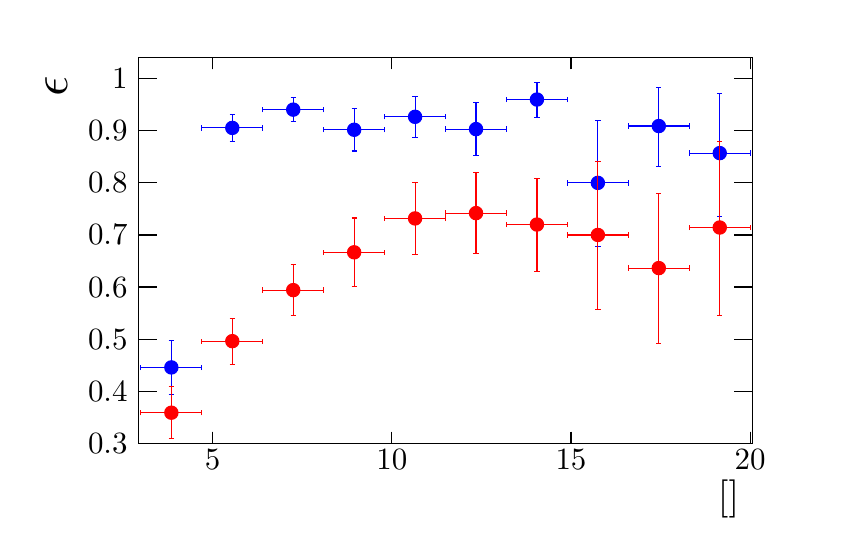
\begin{tikzpicture}
\pgfdeclareplotmark{cross} {
\pgfpathmoveto{\pgfpoint{-0.3\pgfplotmarksize}{\pgfplotmarksize}}
\pgfpathlineto{\pgfpoint{+0.3\pgfplotmarksize}{\pgfplotmarksize}}
\pgfpathlineto{\pgfpoint{+0.3\pgfplotmarksize}{0.3\pgfplotmarksize}}
\pgfpathlineto{\pgfpoint{+1\pgfplotmarksize}{0.3\pgfplotmarksize}}
\pgfpathlineto{\pgfpoint{+1\pgfplotmarksize}{-0.3\pgfplotmarksize}}
\pgfpathlineto{\pgfpoint{+0.3\pgfplotmarksize}{-0.3\pgfplotmarksize}}
\pgfpathlineto{\pgfpoint{+0.3\pgfplotmarksize}{-1.\pgfplotmarksize}}
\pgfpathlineto{\pgfpoint{-0.3\pgfplotmarksize}{-1.\pgfplotmarksize}}
\pgfpathlineto{\pgfpoint{-0.3\pgfplotmarksize}{-0.3\pgfplotmarksize}}
\pgfpathlineto{\pgfpoint{-1.\pgfplotmarksize}{-0.3\pgfplotmarksize}}
\pgfpathlineto{\pgfpoint{-1.\pgfplotmarksize}{0.3\pgfplotmarksize}}
\pgfpathlineto{\pgfpoint{-0.3\pgfplotmarksize}{0.3\pgfplotmarksize}}
\pgfpathclose
\pgfusepathqstroke
}
\pgfdeclareplotmark{cross*} {
\pgfpathmoveto{\pgfpoint{-0.3\pgfplotmarksize}{\pgfplotmarksize}}
\pgfpathlineto{\pgfpoint{+0.3\pgfplotmarksize}{\pgfplotmarksize}}
\pgfpathlineto{\pgfpoint{+0.3\pgfplotmarksize}{0.3\pgfplotmarksize}}
\pgfpathlineto{\pgfpoint{+1\pgfplotmarksize}{0.3\pgfplotmarksize}}
\pgfpathlineto{\pgfpoint{+1\pgfplotmarksize}{-0.3\pgfplotmarksize}}
\pgfpathlineto{\pgfpoint{+0.3\pgfplotmarksize}{-0.3\pgfplotmarksize}}
\pgfpathlineto{\pgfpoint{+0.3\pgfplotmarksize}{-1.\pgfplotmarksize}}
\pgfpathlineto{\pgfpoint{-0.3\pgfplotmarksize}{-1.\pgfplotmarksize}}
\pgfpathlineto{\pgfpoint{-0.3\pgfplotmarksize}{-0.3\pgfplotmarksize}}
\pgfpathlineto{\pgfpoint{-1.\pgfplotmarksize}{-0.3\pgfplotmarksize}}
\pgfpathlineto{\pgfpoint{-1.\pgfplotmarksize}{0.3\pgfplotmarksize}}
\pgfpathlineto{\pgfpoint{-0.3\pgfplotmarksize}{0.3\pgfplotmarksize}}
\pgfpathclose
\pgfusepathqfillstroke
}
\pgfdeclareplotmark{newstar} {
\pgfpathmoveto{\pgfqpoint{0pt}{\pgfplotmarksize}}
\pgfpathlineto{\pgfqpointpolar{44}{0.5\pgfplotmarksize}}
\pgfpathlineto{\pgfqpointpolar{18}{\pgfplotmarksize}}
\pgfpathlineto{\pgfqpointpolar{-20}{0.5\pgfplotmarksize}}
\pgfpathlineto{\pgfqpointpolar{-54}{\pgfplotmarksize}}
\pgfpathlineto{\pgfqpointpolar{-90}{0.5\pgfplotmarksize}}
\pgfpathlineto{\pgfqpointpolar{234}{\pgfplotmarksize}}
\pgfpathlineto{\pgfqpointpolar{198}{0.5\pgfplotmarksize}}
\pgfpathlineto{\pgfqpointpolar{162}{\pgfplotmarksize}}
\pgfpathlineto{\pgfqpointpolar{134}{0.5\pgfplotmarksize}}
\pgfpathclose
\pgfusepathqstroke
}
\pgfdeclareplotmark{newstar*} {
\pgfpathmoveto{\pgfqpoint{0pt}{\pgfplotmarksize}}
\pgfpathlineto{\pgfqpointpolar{44}{0.5\pgfplotmarksize}}
\pgfpathlineto{\pgfqpointpolar{18}{\pgfplotmarksize}}
\pgfpathlineto{\pgfqpointpolar{-20}{0.5\pgfplotmarksize}}
\pgfpathlineto{\pgfqpointpolar{-54}{\pgfplotmarksize}}
\pgfpathlineto{\pgfqpointpolar{-90}{0.5\pgfplotmarksize}}
\pgfpathlineto{\pgfqpointpolar{234}{\pgfplotmarksize}}
\pgfpathlineto{\pgfqpointpolar{198}{0.5\pgfplotmarksize}}
\pgfpathlineto{\pgfqpointpolar{162}{\pgfplotmarksize}}
\pgfpathlineto{\pgfqpointpolar{134}{0.5\pgfplotmarksize}}
\pgfpathclose
\pgfusepathqfillstroke
}
\definecolor{c}{rgb}{1,1,1};
\draw [color=c, fill=c] (0,0) rectangle (10,6.27517);
\draw [color=c, fill=c] (1.4,1.00403) rectangle (9.2,5.89866);
\definecolor{c}{rgb}{0,0,0};
\draw [c] (1.4,1.00403) -- (1.4,5.89866) -- (9.2,5.89866) -- (9.2,1.00403) -- (1.4,1.00403);
\definecolor{c}{rgb}{1,1,1};
\draw [color=c, fill=c] (1.4,1.00403) rectangle (9.2,5.89866);
\definecolor{c}{rgb}{0,0,0};
\draw [c] (1.4,1.00403) -- (1.4,5.89866) -- (9.2,5.89866) -- (9.2,1.00403) -- (1.4,1.00403);
\draw [c,line width=0.4] (1.4,1.00403) -- (9.2,1.00403);
\draw [anchor= east] (9.2,0.301208) node[scale=1.37879, rotate=0]{$\ptot [\gevc]$};
\draw [c,line width=0.4] (2.34132,1.15087) -- (2.34132,1.00403);
\draw [c,line width=0.4] (4.61723,1.15087) -- (4.61723,1.00403);
\draw [c,line width=0.4] (6.89314,1.15087) -- (6.89314,1.00403);
\draw [c,line width=0.4] (9.16905,1.15087) -- (9.16905,1.00403);
\draw [c,line width=0.4] (2.34132,1.15087) -- (2.34132,1.00403);
\draw [c,line width=0.4] (9.16905,1.15087) -- (9.16905,1.00403);
\draw [anchor=base] (2.34132,0.665168) node[scale=1.11794, rotate=0]{5};
\draw [anchor=base] (4.61723,0.665168) node[scale=1.11794, rotate=0]{10};
\draw [anchor=base] (6.89314,0.665168) node[scale=1.11794, rotate=0]{15};
\draw [anchor=base] (9.16905,0.665168) node[scale=1.11794, rotate=0]{20};
\draw [c,line width=0.4] (1.4,5.89866) -- (9.2,5.89866);
\draw [c,line width=0.4] (2.34132,5.75182) -- (2.34132,5.89866);
\draw [c,line width=0.4] (4.61723,5.75182) -- (4.61723,5.89866);
\draw [c,line width=0.4] (6.89314,5.75182) -- (6.89314,5.89866);
\draw [c,line width=0.4] (9.16905,5.75182) -- (9.16905,5.89866);
\draw [c,line width=0.4] (2.34132,5.75182) -- (2.34132,5.89866);
\draw [c,line width=0.4] (9.16905,5.75182) -- (9.16905,5.89866);
\draw [c,line width=0.4] (1.4,1.00403) -- (1.4,5.89866);
\draw [anchor= east] (0.36,5.89866) node[scale=1.82597, rotate=90]{$\epsilon$};
\draw [c,line width=0.4] (1.634,1.00403) -- (1.4,1.00403);
\draw [c,line width=0.4] (1.634,1.66546) -- (1.4,1.66546);
\draw [c,line width=0.4] (1.634,2.3269) -- (1.4,2.3269);
\draw [c,line width=0.4] (1.634,2.98834) -- (1.4,2.98834);
\draw [c,line width=0.4] (1.634,3.64977) -- (1.4,3.64977);
\draw [c,line width=0.4] (1.634,4.31121) -- (1.4,4.31121);
\draw [c,line width=0.4] (1.634,4.97265) -- (1.4,4.97265);
\draw [c,line width=0.4] (1.634,5.63408) -- (1.4,5.63408);
\draw [c,line width=0.4] (1.634,1.00403) -- (1.4,1.00403);
\draw [c,line width=0.4] (1.634,5.63408) -- (1.4,5.63408);
\draw [anchor= east] (1.4,1.00403) node[scale=1.11794, rotate=0]{0.3};
\draw [anchor= east] (1.4,1.66546) node[scale=1.11794, rotate=0]{0.4};
\draw [anchor= east] (1.4,2.3269) node[scale=1.11794, rotate=0]{0.5};
\draw [anchor= east] (1.4,2.98834) node[scale=1.11794, rotate=0]{0.6};
\draw [anchor= east] (1.4,3.64977) node[scale=1.11794, rotate=0]{0.7};
\draw [anchor= east] (1.4,4.31121) node[scale=1.11794, rotate=0]{0.8};
\draw [anchor= east] (1.4,4.97265) node[scale=1.11794, rotate=0]{0.9};
\draw [anchor= east] (1.4,5.63408) node[scale=1.11794, rotate=0]{1};
\draw [c,line width=0.4] (9.2,1.00403) -- (9.2,5.89866);
\draw [c,line width=0.4] (8.966,1.00403) -- (9.2,1.00403);
\draw [c,line width=0.4] (8.966,1.66546) -- (9.2,1.66546);
\draw [c,line width=0.4] (8.966,2.3269) -- (9.2,2.3269);
\draw [c,line width=0.4] (8.966,2.98834) -- (9.2,2.98834);
\draw [c,line width=0.4] (8.966,3.64977) -- (9.2,3.64977);
\draw [c,line width=0.4] (8.966,4.31121) -- (9.2,4.31121);
\draw [c,line width=0.4] (8.966,4.97265) -- (9.2,4.97265);
\draw [c,line width=0.4] (8.966,5.63408) -- (9.2,5.63408);
\draw [c,line width=0.4] (8.966,1.00403) -- (9.2,1.00403);
\draw [c,line width=0.4] (8.966,5.63408) -- (9.2,5.63408);
\definecolor{c}{rgb}{0,0,1};
\foreach \P in {(1.81786,1.96742),(2.59167,5.0091),(3.36548,5.24115),(4.13929,4.98562),(4.9131,5.1501),(5.6869,4.99398),(6.46071,5.36951),(7.23452,4.31121),(8.00833,5.03278),(8.78214,4.68917)}{\draw[mark options={color=c,fill=c},mark
 size=2.402402pt,mark=*] plot coordinates {\P};}
\draw [c,line width=0.4] (1.75074,1.96742) -- (1.43095,1.96742);
\draw [c,line width=0.4] (1.43095,1.93387) -- (1.43095,2.00098);
\draw [c,line width=0.4] (1.88497,1.96742) -- (2.20476,1.96742);
\draw [c,line width=0.4] (2.20476,1.93387) -- (2.20476,2.00098);
\draw [c,line width=0.4] (1.81786,2.03454) -- (1.81786,2.31016);
\draw [c,line width=0.4] (1.7843,2.31016) -- (1.85141,2.31016);
\draw [c,line width=0.4] (1.81786,1.90031) -- (1.81786,1.62472);
\draw [c,line width=0.4] (1.7843,1.62472) -- (1.85141,1.62472);
\draw [c,line width=0.4] (2.52455,5.0091) -- (2.20476,5.0091);
\draw [c,line width=0.4] (2.20476,4.97555) -- (2.20476,5.04266);
\draw [c,line width=0.4] (2.65878,5.0091) -- (2.97857,5.0091);
\draw [c,line width=0.4] (2.97857,4.97555) -- (2.97857,5.04266);
\draw [c,line width=0.4] (2.59167,5.07622) -- (2.59167,5.17895);
\draw [c,line width=0.4] (2.55811,5.17895) -- (2.62522,5.17895);
\draw [c,line width=0.4] (2.59167,4.94199) -- (2.59167,4.83908);
\draw [c,line width=0.4] (2.55811,4.83908) -- (2.62522,4.83908);
\draw [c,line width=0.4] (3.29836,5.24115) -- (2.97857,5.24115);
\draw [c,line width=0.4] (2.97857,5.20759) -- (2.97857,5.27471);
\draw [c,line width=0.4] (3.43259,5.24115) -- (3.75238,5.24115);
\draw [c,line width=0.4] (3.75238,5.20759) -- (3.75238,5.27471);
\draw [c,line width=0.4] (3.36548,5.30826) -- (3.36548,5.39295);
\draw [c,line width=0.4] (3.33192,5.39295) -- (3.39903,5.39295);
\draw [c,line width=0.4] (3.36548,5.17404) -- (3.36548,5.089);
\draw [c,line width=0.4] (3.33192,5.089) -- (3.39903,5.089);
\draw [c,line width=0.4] (4.07217,4.98562) -- (3.75238,4.98562);
\draw [c,line width=0.4] (3.75238,4.95206) -- (3.75238,5.01917);
\draw [c,line width=0.4] (4.2064,4.98562) -- (4.52619,4.98562);
\draw [c,line width=0.4] (4.52619,4.95206) -- (4.52619,5.01917);
\draw [c,line width=0.4] (4.13929,5.05273) -- (4.13929,5.25381);
\draw [c,line width=0.4] (4.10573,5.25381) -- (4.17284,5.25381);
\draw [c,line width=0.4] (4.13929,4.9185) -- (4.13929,4.71636);
\draw [c,line width=0.4] (4.10573,4.71636) -- (4.17284,4.71636);
\draw [c,line width=0.4] (4.84598,5.1501) -- (4.52619,5.1501);
\draw [c,line width=0.4] (4.52619,5.11655) -- (4.52619,5.18366);
\draw [c,line width=0.4] (4.98021,5.1501) -- (5.3,5.1501);
\draw [c,line width=0.4] (5.3,5.11655) -- (5.3,5.18366);
\draw [c,line width=0.4] (4.9131,5.21722) -- (4.9131,5.40614);
\draw [c,line width=0.4] (4.87954,5.40614) -- (4.94665,5.40614);
\draw [c,line width=0.4] (4.9131,5.08299) -- (4.9131,4.89215);
\draw [c,line width=0.4] (4.87954,4.89215) -- (4.94665,4.89215);
\draw [c,line width=0.4] (5.61979,4.99398) -- (5.3,4.99398);
\draw [c,line width=0.4] (5.3,4.96043) -- (5.3,5.02754);
\draw [c,line width=0.4] (5.75402,4.99398) -- (6.07381,4.99398);
\draw [c,line width=0.4] (6.07381,4.96043) -- (6.07381,5.02754);
\draw [c,line width=0.4] (5.6869,5.0611) -- (5.6869,5.32931);
\draw [c,line width=0.4] (5.65335,5.32931) -- (5.72046,5.32931);
\draw [c,line width=0.4] (5.6869,4.92687) -- (5.6869,4.65575);
\draw [c,line width=0.4] (5.65335,4.65575) -- (5.72046,4.65575);
\draw [c,line width=0.4] (6.3936,5.36951) -- (6.07381,5.36951);
\draw [c,line width=0.4] (6.07381,5.33595) -- (6.07381,5.40307);
\draw [c,line width=0.4] (6.52783,5.36951) -- (6.84762,5.36951);
\draw [c,line width=0.4] (6.84762,5.33595) -- (6.84762,5.40307);
\draw [c,line width=0.4] (6.46071,5.43662) -- (6.46071,5.58664);
\draw [c,line width=0.4] (6.42716,5.58664) -- (6.49427,5.58664);
\draw [c,line width=0.4] (6.46071,5.30239) -- (6.46071,5.14567);
\draw [c,line width=0.4] (6.42716,5.14567) -- (6.49427,5.14567);
\draw [c,line width=0.4] (7.16741,4.31121) -- (6.84762,4.31121);
\draw [c,line width=0.4] (6.84762,4.27765) -- (6.84762,4.34477);
\draw [c,line width=0.4] (7.30164,4.31121) -- (7.62143,4.31121);
\draw [c,line width=0.4] (7.62143,4.27765) -- (7.62143,4.34477);
\draw [c,line width=0.4] (7.23452,4.37832) -- (7.23452,5.10425);
\draw [c,line width=0.4] (7.20097,5.10425) -- (7.26808,5.10425);
\draw [c,line width=0.4] (7.23452,4.2441) -- (7.23452,3.49983);
\draw [c,line width=0.4] (7.20097,3.49983) -- (7.26808,3.49983);
\draw [c,line width=0.4] (7.94122,5.03278) -- (7.62143,5.03278);
\draw [c,line width=0.4] (7.62143,4.99922) -- (7.62143,5.06633);
\draw [c,line width=0.4] (8.07545,5.03278) -- (8.39524,5.03278);
\draw [c,line width=0.4] (8.39524,4.99922) -- (8.39524,5.06633);
\draw [c,line width=0.4] (8.00833,5.09989) -- (8.00833,5.5208);
\draw [c,line width=0.4] (7.97478,5.5208) -- (8.04189,5.5208);
\draw [c,line width=0.4] (8.00833,4.96566) -- (8.00833,4.52188);
\draw [c,line width=0.4] (7.97478,4.52188) -- (8.04189,4.52188);
\draw [c,line width=0.4] (8.71503,4.68917) -- (8.39524,4.68917);
\draw [c,line width=0.4] (8.39524,4.65562) -- (8.39524,4.72273);
\draw [c,line width=0.4] (8.84926,4.68917) -- (9.16905,4.68917);
\draw [c,line width=0.4] (9.16905,4.65562) -- (9.16905,4.72273);
\draw [c,line width=0.4] (8.78214,4.75629) -- (8.78214,5.44636);
\draw [c,line width=0.4] (8.74859,5.44636) -- (8.8157,5.44636);
\draw [c,line width=0.4] (8.78214,4.62206) -- (8.78214,3.88637);
\draw [c,line width=0.4] (8.74859,3.88637) -- (8.8157,3.88637);
\definecolor{c}{rgb}{1,0,0};
\draw [c,line width=0.4] (1.75074,1.39226) -- (1.43095,1.39226);
\draw [c,line width=0.4] (1.43095,1.3587) -- (1.43095,1.42582);
\draw [c,line width=0.4] (1.88497,1.39226) -- (2.20476,1.39226);
\draw [c,line width=0.4] (2.20476,1.3587) -- (2.20476,1.42582);
\draw [c,line width=0.4] (1.81786,1.45938) -- (1.81786,1.72283);
\draw [c,line width=0.4] (1.7843,1.72283) -- (1.85141,1.72283);
\draw [c,line width=0.4] (1.81786,1.32515) -- (1.81786,1.06178);
\draw [c,line width=0.4] (1.7843,1.06178) -- (1.85141,1.06178);
\draw [c,line width=0.4] (2.52455,2.30086) -- (2.20476,2.30086);
\draw [c,line width=0.4] (2.20476,2.2673) -- (2.20476,2.33442);
\draw [c,line width=0.4] (2.65878,2.30086) -- (2.97857,2.30086);
\draw [c,line width=0.4] (2.97857,2.2673) -- (2.97857,2.33442);
\draw [c,line width=0.4] (2.59167,2.36797) -- (2.59167,2.59431);
\draw [c,line width=0.4] (2.55811,2.59431) -- (2.62522,2.59431);
\draw [c,line width=0.4] (2.59167,2.23375) -- (2.59167,2.00741);
\draw [c,line width=0.4] (2.55811,2.00741) -- (2.62522,2.00741);
\draw [c,line width=0.4] (3.29836,2.94904) -- (2.97857,2.94904);
\draw [c,line width=0.4] (2.97857,2.91549) -- (2.97857,2.9826);
\draw [c,line width=0.4] (3.43259,2.94904) -- (3.75238,2.94904);
\draw [c,line width=0.4] (3.75238,2.91549) -- (3.75238,2.9826);
\draw [c,line width=0.4] (3.36548,3.01616) -- (3.36548,3.27214);
\draw [c,line width=0.4] (3.33192,3.27214) -- (3.39903,3.27214);
\draw [c,line width=0.4] (3.36548,2.88193) -- (3.36548,2.6259);
\draw [c,line width=0.4] (3.33192,2.6259) -- (3.39903,2.6259);
\draw [c,line width=0.4] (4.07217,3.42929) -- (3.75238,3.42929);
\draw [c,line width=0.4] (3.75238,3.39574) -- (3.75238,3.46285);
\draw [c,line width=0.4] (4.2064,3.42929) -- (4.52619,3.42929);
\draw [c,line width=0.4] (4.52619,3.39574) -- (4.52619,3.46285);
\draw [c,line width=0.4] (4.13929,3.49641) -- (4.13929,3.86499);
\draw [c,line width=0.4] (4.10573,3.86499) -- (4.17284,3.86499);
\draw [c,line width=0.4] (4.13929,3.36218) -- (4.13929,2.99325);
\draw [c,line width=0.4] (4.10573,2.99325) -- (4.17284,2.99325);
\draw [c,line width=0.4] (4.84598,3.8595) -- (4.52619,3.8595);
\draw [c,line width=0.4] (4.52619,3.82594) -- (4.52619,3.89305);
\draw [c,line width=0.4] (4.98021,3.8595) -- (5.3,3.8595);
\draw [c,line width=0.4] (5.3,3.82594) -- (5.3,3.89305);
\draw [c,line width=0.4] (4.9131,3.92661) -- (4.9131,4.31469);
\draw [c,line width=0.4] (4.87954,4.31469) -- (4.94665,4.31469);
\draw [c,line width=0.4] (4.9131,3.79238) -- (4.9131,3.40353);
\draw [c,line width=0.4] (4.87954,3.40353) -- (4.94665,3.40353);
\draw [c,line width=0.4] (5.61979,3.92715) -- (5.3,3.92715);
\draw [c,line width=0.4] (5.3,3.89359) -- (5.3,3.96071);
\draw [c,line width=0.4] (5.75402,3.92715) -- (6.07381,3.92715);
\draw [c,line width=0.4] (6.07381,3.89359) -- (6.07381,3.96071);
\draw [c,line width=0.4] (5.6869,3.99426) -- (5.6869,4.44269);
\draw [c,line width=0.4] (5.65335,4.44269) -- (5.72046,4.44269);
\draw [c,line width=0.4] (5.6869,3.86004) -- (5.6869,3.41018);
\draw [c,line width=0.4] (5.65335,3.41018) -- (5.72046,3.41018);
\draw [c,line width=0.4] (6.3936,3.78206) -- (6.07381,3.78206);
\draw [c,line width=0.4] (6.07381,3.7485) -- (6.07381,3.81562);
\draw [c,line width=0.4] (6.52783,3.78206) -- (6.84762,3.78206);
\draw [c,line width=0.4] (6.84762,3.7485) -- (6.84762,3.81562);
\draw [c,line width=0.4] (6.46071,3.84917) -- (6.46071,4.371);
\draw [c,line width=0.4] (6.42716,4.371) -- (6.49427,4.371);
\draw [c,line width=0.4] (6.46071,3.71495) -- (6.46071,3.19113);
\draw [c,line width=0.4] (6.42716,3.19113) -- (6.49427,3.19113);
\draw [c,line width=0.4] (7.16741,3.64977) -- (6.84762,3.64977);
\draw [c,line width=0.4] (6.84762,3.61622) -- (6.84762,3.68333);
\draw [c,line width=0.4] (7.30164,3.64977) -- (7.62143,3.64977);
\draw [c,line width=0.4] (7.62143,3.61622) -- (7.62143,3.68333);
\draw [c,line width=0.4] (7.23452,3.71689) -- (7.23452,4.5882);
\draw [c,line width=0.4] (7.20097,4.5882) -- (7.26808,4.5882);
\draw [c,line width=0.4] (7.23452,3.58266) -- (7.23452,2.69961);
\draw [c,line width=0.4] (7.20097,2.69961) -- (7.26808,2.69961);
\draw [c,line width=0.4] (7.94122,3.22886) -- (7.62143,3.22886);
\draw [c,line width=0.4] (7.62143,3.1953) -- (7.62143,3.26242);
\draw [c,line width=0.4] (8.07545,3.22886) -- (8.39524,3.22886);
\draw [c,line width=0.4] (8.39524,3.1953) -- (8.39524,3.26242);
\draw [c,line width=0.4] (8.00833,3.29597) -- (8.00833,4.17898);
\draw [c,line width=0.4] (7.97478,4.17898) -- (8.04189,4.17898);
\draw [c,line width=0.4] (8.00833,3.16175) -- (8.00833,2.27225);
\draw [c,line width=0.4] (7.97478,2.27225) -- (8.04189,2.27225);
\draw [c,line width=0.4] (8.71503,3.74426) -- (8.39524,3.74426);
\draw [c,line width=0.4] (8.39524,3.71071) -- (8.39524,3.77782);
\draw [c,line width=0.4] (8.84926,3.74426) -- (9.16905,3.74426);
\draw [c,line width=0.4] (9.16905,3.71071) -- (9.16905,3.77782);
\draw [c,line width=0.4] (8.78214,3.81138) -- (8.78214,4.83111);
\draw [c,line width=0.4] (8.74859,4.83111) -- (8.8157,4.83111);
\draw [c,line width=0.4] (8.78214,3.67715) -- (8.78214,2.63105);
\draw [c,line width=0.4] (8.74859,2.63105) -- (8.8157,2.63105);
\foreach \P in {(1.81786,1.39226),(2.59167,2.30086),(3.36548,2.94904),(4.13929,3.42929),(4.9131,3.8595),(5.6869,3.92715),(6.46071,3.78206),(7.23452,3.64977),(8.00833,3.22886),(8.78214,3.74426)}{\draw[mark options={color=c,fill=c},mark
 size=2.402402pt,mark=*] plot coordinates {\P};}
\end{tikzpicture}
}
  \caption{Efficiency comparison between the old (red) and new (blue) matching algorithms in bins of total momentum.}
 \label{mvm_eff_p_comp}
\end{figure}

After the improvements mentioned in the above paragraph the efficiency of the upgraded \mvTTm algorithm
is estimated using simulated \Sigmapmumu events, where the mean transverse momentum is $\sim 300\mevc$.
The muons from this decay, which passed the full track reconstruction resulting in Long tracks,
are further ensured to be muons. This is possible by exploiting the available information in the
simulated event and thus defining the {\it true muons}.
An important concept that is used for the \mvTTm efficiency definition is the so called {\it overlap}.
Specifically, a certain \velo track overlaps with a true muon (which is a Long track)
when the \velo track has more than $70\%$ \velo hits in common with the \velo segment
of the true muon track. The number of all \veloTTracks that overlap with a true muon define the
denominator in the \mvTTm efficiency, while these \veloTTracks that are in addition accepted by
the \mvTTm algorithm make the number in the numerator.

The efficiency is compared against the old
\mvm algorithm, where a common cutoff value for the $\chisq/\nDoF$ of 2 is chosen. The efficiency
versus the total momentum, can be seen in \figref{mvm_eff_p_comp}, where the improvement of the
upgraded \mvTTm algorithm is shown to be significant.  Given that the aim of the \mvTTm upgrade
is to optimize for high efficiency of low transverse momenta muons the efficiency is also projected
versus $\pt$ and shown in \figref{mvm_eff_pt_zoom_comp}. As mentioned in \secref{muid_hlt1}, the
high $\pt$ muons will not be processed by the \mvTTm algorithm and thus the previous figure focuses on
the region where $\pt\in[0,0.5]\gevc$. The relative efficiency increase with respect to the old
\mvm algorithm in the above region is $\sim 50\%$. Finally, the improvement of the $\chisq/\nDoF$
discriminating power between the old and upgraded algorithm is shown in \figref{mvm_chi2_comp}.

\begin{figure}[t]
  \centering
  \begin{subfigure}{0.5\textwidth}
    \raggedright
    \tikzsetnextfilename{mvm_chi2_sigpt_smaller}
    \scalebox{.55}{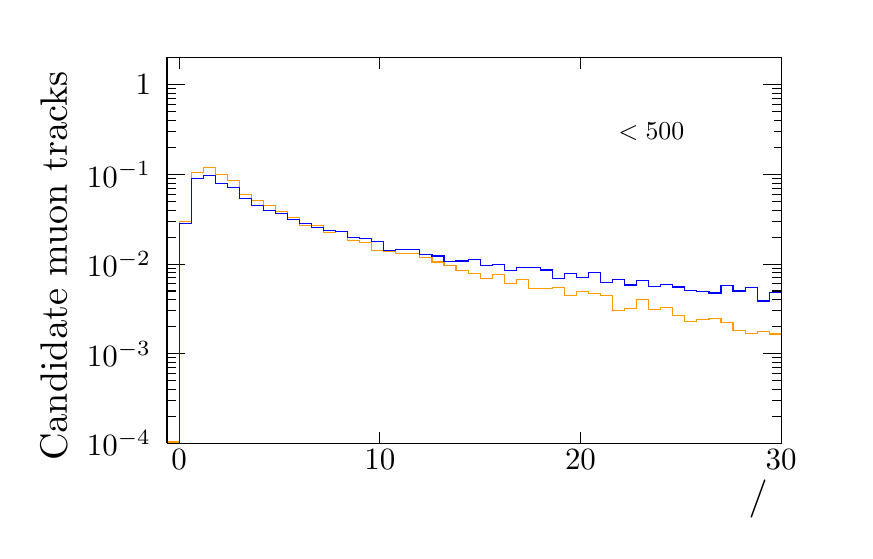
\begin{tikzpicture}
\pgfdeclareplotmark{cross} {
\pgfpathmoveto{\pgfpoint{-0.3\pgfplotmarksize}{\pgfplotmarksize}}
\pgfpathlineto{\pgfpoint{+0.3\pgfplotmarksize}{\pgfplotmarksize}}
\pgfpathlineto{\pgfpoint{+0.3\pgfplotmarksize}{0.3\pgfplotmarksize}}
\pgfpathlineto{\pgfpoint{+1\pgfplotmarksize}{0.3\pgfplotmarksize}}
\pgfpathlineto{\pgfpoint{+1\pgfplotmarksize}{-0.3\pgfplotmarksize}}
\pgfpathlineto{\pgfpoint{+0.3\pgfplotmarksize}{-0.3\pgfplotmarksize}}
\pgfpathlineto{\pgfpoint{+0.3\pgfplotmarksize}{-1.\pgfplotmarksize}}
\pgfpathlineto{\pgfpoint{-0.3\pgfplotmarksize}{-1.\pgfplotmarksize}}
\pgfpathlineto{\pgfpoint{-0.3\pgfplotmarksize}{-0.3\pgfplotmarksize}}
\pgfpathlineto{\pgfpoint{-1.\pgfplotmarksize}{-0.3\pgfplotmarksize}}
\pgfpathlineto{\pgfpoint{-1.\pgfplotmarksize}{0.3\pgfplotmarksize}}
\pgfpathlineto{\pgfpoint{-0.3\pgfplotmarksize}{0.3\pgfplotmarksize}}
\pgfpathclose
\pgfusepathqstroke
}
\pgfdeclareplotmark{cross*} {
\pgfpathmoveto{\pgfpoint{-0.3\pgfplotmarksize}{\pgfplotmarksize}}
\pgfpathlineto{\pgfpoint{+0.3\pgfplotmarksize}{\pgfplotmarksize}}
\pgfpathlineto{\pgfpoint{+0.3\pgfplotmarksize}{0.3\pgfplotmarksize}}
\pgfpathlineto{\pgfpoint{+1\pgfplotmarksize}{0.3\pgfplotmarksize}}
\pgfpathlineto{\pgfpoint{+1\pgfplotmarksize}{-0.3\pgfplotmarksize}}
\pgfpathlineto{\pgfpoint{+0.3\pgfplotmarksize}{-0.3\pgfplotmarksize}}
\pgfpathlineto{\pgfpoint{+0.3\pgfplotmarksize}{-1.\pgfplotmarksize}}
\pgfpathlineto{\pgfpoint{-0.3\pgfplotmarksize}{-1.\pgfplotmarksize}}
\pgfpathlineto{\pgfpoint{-0.3\pgfplotmarksize}{-0.3\pgfplotmarksize}}
\pgfpathlineto{\pgfpoint{-1.\pgfplotmarksize}{-0.3\pgfplotmarksize}}
\pgfpathlineto{\pgfpoint{-1.\pgfplotmarksize}{0.3\pgfplotmarksize}}
\pgfpathlineto{\pgfpoint{-0.3\pgfplotmarksize}{0.3\pgfplotmarksize}}
\pgfpathclose
\pgfusepathqfillstroke
}
\pgfdeclareplotmark{newstar} {
\pgfpathmoveto{\pgfqpoint{0pt}{\pgfplotmarksize}}
\pgfpathlineto{\pgfqpointpolar{44}{0.5\pgfplotmarksize}}
\pgfpathlineto{\pgfqpointpolar{18}{\pgfplotmarksize}}
\pgfpathlineto{\pgfqpointpolar{-20}{0.5\pgfplotmarksize}}
\pgfpathlineto{\pgfqpointpolar{-54}{\pgfplotmarksize}}
\pgfpathlineto{\pgfqpointpolar{-90}{0.5\pgfplotmarksize}}
\pgfpathlineto{\pgfqpointpolar{234}{\pgfplotmarksize}}
\pgfpathlineto{\pgfqpointpolar{198}{0.5\pgfplotmarksize}}
\pgfpathlineto{\pgfqpointpolar{162}{\pgfplotmarksize}}
\pgfpathlineto{\pgfqpointpolar{134}{0.5\pgfplotmarksize}}
\pgfpathclose
\pgfusepathqstroke
}
\pgfdeclareplotmark{newstar*} {
\pgfpathmoveto{\pgfqpoint{0pt}{\pgfplotmarksize}}
\pgfpathlineto{\pgfqpointpolar{44}{0.5\pgfplotmarksize}}
\pgfpathlineto{\pgfqpointpolar{18}{\pgfplotmarksize}}
\pgfpathlineto{\pgfqpointpolar{-20}{0.5\pgfplotmarksize}}
\pgfpathlineto{\pgfqpointpolar{-54}{\pgfplotmarksize}}
\pgfpathlineto{\pgfqpointpolar{-90}{0.5\pgfplotmarksize}}
\pgfpathlineto{\pgfqpointpolar{234}{\pgfplotmarksize}}
\pgfpathlineto{\pgfqpointpolar{198}{0.5\pgfplotmarksize}}
\pgfpathlineto{\pgfqpointpolar{162}{\pgfplotmarksize}}
\pgfpathlineto{\pgfqpointpolar{134}{0.5\pgfplotmarksize}}
\pgfpathclose
\pgfusepathqfillstroke
}
\definecolor{c}{rgb}{1,1,1};
\draw [color=c, fill=c] (0,0) rectangle (10,6.27517);
\draw [color=c, fill=c] (1.4,1.00403) rectangle (9.2,5.89866);
\definecolor{c}{rgb}{0,0,0};
\draw [c] (1.4,1.00403) -- (1.4,5.89866) -- (9.2,5.89866) -- (9.2,1.00403) -- (1.4,1.00403);
\definecolor{c}{rgb}{1,1,1};
\draw [color=c, fill=c] (1.4,1.00403) rectangle (9.2,5.89866);
\definecolor{c}{rgb}{0,0,0};
\draw [c] (1.4,1.00403) -- (1.4,5.89866) -- (9.2,5.89866) -- (9.2,1.00403) -- (1.4,1.00403);
\definecolor{c}{rgb}{1,0.6,0};
\draw [c,line width=0.4] (1.41678,1.02081) -- (1.41678,1.02081) -- (1.55294,1.02081) -- (1.55294,3.82277) -- (1.70588,3.82277) -- (1.70588,4.43859) -- (1.85882,4.43859) -- (1.85882,4.50284) -- (2.01176,4.50284) -- (2.01176,4.41416) --
 (2.16471,4.41416) -- (2.16471,4.3398) -- (2.31765,4.3398) -- (2.31765,4.16077) -- (2.47059,4.16077) -- (2.47059,4.08455) -- (2.62353,4.08455) -- (2.62353,4.0208) -- (2.77647,4.0208) -- (2.77647,3.95189) -- (2.92941,3.95189) -- (2.92941,3.8718) --
 (3.08235,3.8718) -- (3.08235,3.77058) -- (3.23529,3.77058) -- (3.23529,3.77338) -- (3.38824,3.77338) -- (3.38824,3.68092) -- (3.54118,3.68092) -- (3.54118,3.68894) -- (3.69412,3.68894) -- (3.69412,3.57799) -- (3.84706,3.57799) -- (3.84706,3.55246)
 -- (4,3.55246) -- (4,3.45638) -- (4.15294,3.45638) -- (4.15294,3.44021) -- (4.30588,3.44021) -- (4.30588,3.41202) -- (4.45882,3.41202) -- (4.45882,3.41086) -- (4.61176,3.41086) -- (4.61176,3.36201) -- (4.76471,3.36201) -- (4.76471,3.30636) --
 (4.91765,3.30636) -- (4.91765,3.26126) -- (5.07059,3.26126) -- (5.07059,3.19751) -- (5.22353,3.19751) -- (5.22353,3.16418) -- (5.37647,3.16418) -- (5.37647,3.09212) -- (5.52941,3.09212) -- (5.52941,3.14861) -- (5.68235,3.14861) -- (5.68235,3.02834)
 -- (5.83529,3.02834) -- (5.83529,3.08318) -- (5.98824,3.08318) -- (5.98824,2.97233) -- (6.14118,2.97233) -- (6.14118,2.96665) -- (6.29412,2.96665) -- (6.29412,2.98073) -- (6.44706,2.98073) -- (6.44706,2.88616) -- (6.6,2.88616) -- (6.6,2.93722) --
 (6.75294,2.93722) -- (6.75294,2.90269) -- (6.90588,2.90269) -- (6.90588,2.88278) -- (7.05882,2.88278) -- (7.05882,2.69575) -- (7.21176,2.69575) -- (7.21176,2.71986) -- (7.36471,2.71986) -- (7.36471,2.8292) -- (7.51765,2.8292) -- (7.51765,2.70067) --
 (7.67059,2.70067) -- (7.67059,2.72919) -- (7.82353,2.72919) -- (7.82353,2.62692) -- (7.97647,2.62692) -- (7.97647,2.55357) -- (8.12941,2.55357) -- (8.12941,2.57925) -- (8.28235,2.57925) -- (8.28235,2.58546) -- (8.43529,2.58546) -- (8.43529,2.54021)
 -- (8.58823,2.54021) -- (8.58823,2.43497) -- (8.74118,2.43497) -- (8.74118,2.40028) -- (8.89412,2.40028) -- (8.89412,2.42653) -- (9.04706,2.42653) -- (9.04706,2.39121) -- (9.2,2.39121) -- (9.2,1.02081);
\definecolor{c}{rgb}{0,0,0};
\draw [c,line width=0.4] (1.4,1.00403) -- (9.2,1.00403);
\draw [anchor= east] (9.2,0.301208) node[scale=1.37879, rotate=0]{$\chisq/\nDoF$};
\draw [c,line width=0.4] (1.55294,1.15087) -- (1.55294,1.00403);
\draw [c,line width=0.4] (4.10196,1.15087) -- (4.10196,1.00403);
\draw [c,line width=0.4] (6.65098,1.15087) -- (6.65098,1.00403);
\draw [c,line width=0.4] (9.2,1.15087) -- (9.2,1.00403);
\draw [c,line width=0.4] (1.55294,1.15087) -- (1.55294,1.00403);
\draw [anchor=base] (1.55294,0.665168) node[scale=1.11794, rotate=0]{0};
\draw [anchor=base] (4.10196,0.665168) node[scale=1.11794, rotate=0]{10};
\draw [anchor=base] (6.65098,0.665168) node[scale=1.11794, rotate=0]{20};
\draw [anchor=base] (9.2,0.665168) node[scale=1.11794, rotate=0]{30};
\draw [c,line width=0.4] (1.4,5.89866) -- (9.2,5.89866);
\draw [c,line width=0.4] (1.55294,5.75182) -- (1.55294,5.89866);
\draw [c,line width=0.4] (4.10196,5.75182) -- (4.10196,5.89866);
\draw [c,line width=0.4] (6.65098,5.75182) -- (6.65098,5.89866);
\draw [c,line width=0.4] (9.2,5.75182) -- (9.2,5.89866);
\draw [c,line width=0.4] (1.55294,5.75182) -- (1.55294,5.89866);
\draw [c,line width=0.4] (1.4,1.00403) -- (1.4,5.89866);
\draw [anchor= east] (-0.04,5.89866) node[scale=1.37879, rotate=90]{Candidate muon tracks};
\draw [c,line width=0.4] (1.634,1.00403) -- (1.4,1.00403);
\draw [anchor= east] (1.336,1.00403) node[scale=1.11794, rotate=0]{$10^{-4}$};
\draw [c,line width=0.4] (1.517,1.3466) -- (1.4,1.3466);
\draw [c,line width=0.4] (1.517,1.547) -- (1.4,1.547);
\draw [c,line width=0.4] (1.517,1.68918) -- (1.4,1.68918);
\draw [c,line width=0.4] (1.517,1.79947) -- (1.4,1.79947);
\draw [c,line width=0.4] (1.517,1.88957) -- (1.4,1.88957);
\draw [c,line width=0.4] (1.517,1.96576) -- (1.4,1.96576);
\draw [c,line width=0.4] (1.517,2.03176) -- (1.4,2.03176);
\draw [c,line width=0.4] (1.517,2.08997) -- (1.4,2.08997);
\draw [c,line width=0.4] (1.634,2.14204) -- (1.4,2.14204);
\draw [anchor= east] (1.336,2.14204) node[scale=1.11794, rotate=0]{$10^{-3}$};
\draw [c,line width=0.4] (1.517,2.48462) -- (1.4,2.48462);
\draw [c,line width=0.4] (1.517,2.68501) -- (1.4,2.68501);
\draw [c,line width=0.4] (1.517,2.82719) -- (1.4,2.82719);
\draw [c,line width=0.4] (1.517,2.93748) -- (1.4,2.93748);
\draw [c,line width=0.4] (1.517,3.02759) -- (1.4,3.02759);
\draw [c,line width=0.4] (1.517,3.10377) -- (1.4,3.10377);
\draw [c,line width=0.4] (1.517,3.16977) -- (1.4,3.16977);
\draw [c,line width=0.4] (1.517,3.22798) -- (1.4,3.22798);
\draw [c,line width=0.4] (1.634,3.28005) -- (1.4,3.28005);
\draw [anchor= east] (1.336,3.28005) node[scale=1.11794, rotate=0]{$10^{-2}$};
\draw [c,line width=0.4] (1.517,3.62263) -- (1.4,3.62263);
\draw [c,line width=0.4] (1.517,3.82303) -- (1.4,3.82303);
\draw [c,line width=0.4] (1.517,3.96521) -- (1.4,3.96521);
\draw [c,line width=0.4] (1.517,4.07549) -- (1.4,4.07549);
\draw [c,line width=0.4] (1.517,4.1656) -- (1.4,4.1656);
\draw [c,line width=0.4] (1.517,4.24179) -- (1.4,4.24179);
\draw [c,line width=0.4] (1.517,4.30778) -- (1.4,4.30778);
\draw [c,line width=0.4] (1.517,4.366) -- (1.4,4.366);
\draw [c,line width=0.4] (1.634,4.41807) -- (1.4,4.41807);
\draw [anchor= east] (1.336,4.41807) node[scale=1.11794, rotate=0]{$10^{-1}$};
\draw [c,line width=0.4] (1.517,4.76064) -- (1.4,4.76064);
\draw [c,line width=0.4] (1.517,4.96104) -- (1.4,4.96104);
\draw [c,line width=0.4] (1.517,5.10322) -- (1.4,5.10322);
\draw [c,line width=0.4] (1.517,5.21351) -- (1.4,5.21351);
\draw [c,line width=0.4] (1.517,5.30361) -- (1.4,5.30361);
\draw [c,line width=0.4] (1.517,5.3798) -- (1.4,5.3798);
\draw [c,line width=0.4] (1.517,5.4458) -- (1.4,5.4458);
\draw [c,line width=0.4] (1.517,5.50401) -- (1.4,5.50401);
\draw [c,line width=0.4] (1.634,5.55608) -- (1.4,5.55608);
\draw [anchor= east] (1.336,5.55608) node[scale=1.11794, rotate=0]{1};
\draw [c,line width=0.4] (1.517,5.89866) -- (1.4,5.89866);
\draw [c,line width=0.4] (9.2,1.00403) -- (9.2,5.89866);
\draw [c,line width=0.4] (8.966,1.00403) -- (9.2,1.00403);
\draw [c,line width=0.4] (9.083,1.3466) -- (9.2,1.3466);
\draw [c,line width=0.4] (9.083,1.547) -- (9.2,1.547);
\draw [c,line width=0.4] (9.083,1.68918) -- (9.2,1.68918);
\draw [c,line width=0.4] (9.083,1.79947) -- (9.2,1.79947);
\draw [c,line width=0.4] (9.083,1.88957) -- (9.2,1.88957);
\draw [c,line width=0.4] (9.083,1.96576) -- (9.2,1.96576);
\draw [c,line width=0.4] (9.083,2.03176) -- (9.2,2.03176);
\draw [c,line width=0.4] (9.083,2.08997) -- (9.2,2.08997);
\draw [c,line width=0.4] (8.966,2.14204) -- (9.2,2.14204);
\draw [c,line width=0.4] (9.083,2.48462) -- (9.2,2.48462);
\draw [c,line width=0.4] (9.083,2.68501) -- (9.2,2.68501);
\draw [c,line width=0.4] (9.083,2.82719) -- (9.2,2.82719);
\draw [c,line width=0.4] (9.083,2.93748) -- (9.2,2.93748);
\draw [c,line width=0.4] (9.083,3.02759) -- (9.2,3.02759);
\draw [c,line width=0.4] (9.083,3.10377) -- (9.2,3.10377);
\draw [c,line width=0.4] (9.083,3.16977) -- (9.2,3.16977);
\draw [c,line width=0.4] (9.083,3.22798) -- (9.2,3.22798);
\draw [c,line width=0.4] (8.966,3.28005) -- (9.2,3.28005);
\draw [c,line width=0.4] (9.083,3.62263) -- (9.2,3.62263);
\draw [c,line width=0.4] (9.083,3.82303) -- (9.2,3.82303);
\draw [c,line width=0.4] (9.083,3.96521) -- (9.2,3.96521);
\draw [c,line width=0.4] (9.083,4.07549) -- (9.2,4.07549);
\draw [c,line width=0.4] (9.083,4.1656) -- (9.2,4.1656);
\draw [c,line width=0.4] (9.083,4.24179) -- (9.2,4.24179);
\draw [c,line width=0.4] (9.083,4.30778) -- (9.2,4.30778);
\draw [c,line width=0.4] (9.083,4.366) -- (9.2,4.366);
\draw [c,line width=0.4] (8.966,4.41807) -- (9.2,4.41807);
\draw [c,line width=0.4] (9.083,4.76064) -- (9.2,4.76064);
\draw [c,line width=0.4] (9.083,4.96104) -- (9.2,4.96104);
\draw [c,line width=0.4] (9.083,5.10322) -- (9.2,5.10322);
\draw [c,line width=0.4] (9.083,5.21351) -- (9.2,5.21351);
\draw [c,line width=0.4] (9.083,5.30361) -- (9.2,5.30361);
\draw [c,line width=0.4] (9.083,5.3798) -- (9.2,5.3798);
\draw [c,line width=0.4] (9.083,5.4458) -- (9.2,5.4458);
\draw [c,line width=0.4] (9.083,5.50401) -- (9.2,5.50401);
\draw [c,line width=0.4] (8.966,5.55608) -- (9.2,5.55608);
\draw [c,line width=0.4] (9.083,5.89866) -- (9.2,5.89866);
\definecolor{c}{rgb}{0,0,1};
\draw [c,line width=0.4] (1.55294,1.02081) -- (1.55294,3.79674) -- (1.70588,3.79674) -- (1.70588,4.36712) -- (1.85882,4.36712) -- (1.85882,4.40799) -- (2.01176,4.40799) -- (2.01176,4.30465) -- (2.16471,4.30465) -- (2.16471,4.2558) -- (2.31765,4.2558)
 -- (2.31765,4.11481) -- (2.47059,4.11481) -- (2.47059,4.01966) -- (2.62353,4.01966) -- (2.62353,3.96151) -- (2.77647,3.96151) -- (2.77647,3.92204) -- (2.92941,3.92204) -- (2.92941,3.84845) -- (3.08235,3.84845) -- (3.08235,3.78957) --
 (3.23529,3.78957) -- (3.23529,3.74471) -- (3.38824,3.74471) -- (3.38824,3.70354) -- (3.54118,3.70354) -- (3.54118,3.69922) -- (3.69412,3.69922) -- (3.69412,3.62063) -- (3.84706,3.62063) -- (3.84706,3.59989) -- (4,3.59989) -- (4,3.56389) --
 (4.15294,3.56389) -- (4.15294,3.4474) -- (4.30588,3.4474) -- (4.30588,3.46857) -- (4.45882,3.46857) -- (4.45882,3.46083) -- (4.61176,3.46083) -- (4.61176,3.39595) -- (4.76471,3.39595) -- (4.76471,3.38243) -- (4.91765,3.38243) -- (4.91765,3.31604) --
 (5.07059,3.31604) -- (5.07059,3.31917) -- (5.22353,3.31917) -- (5.22353,3.33249) -- (5.37647,3.33249) -- (5.37647,3.25966) -- (5.52941,3.25966) -- (5.52941,3.27918) -- (5.68235,3.27918) -- (5.68235,3.19998) -- (5.83529,3.19998) -- (5.83529,3.23566)
 -- (5.98824,3.23566) -- (5.98824,3.23072) -- (6.14118,3.23072) -- (6.14118,3.20524) -- (6.29412,3.20524) -- (6.29412,3.09918) -- (6.44706,3.09918) -- (6.44706,3.16295) -- (6.6,3.16295) -- (6.6,3.11356) -- (6.75294,3.11356) -- (6.75294,3.17282) --
 (6.90588,3.17282) -- (6.90588,3.0444) -- (7.05882,3.0444) -- (7.05882,3.08438) -- (7.21176,3.08438) -- (7.21176,3.01455) -- (7.36471,3.01455) -- (7.36471,3.06912) -- (7.51765,3.06912) -- (7.51765,2.99892) -- (7.67059,2.99892) -- (7.67059,3.01647) --
 (7.82353,3.01647) -- (7.82353,2.9889) -- (7.97647,2.9889) -- (7.97647,2.94663) -- (8.12941,2.94663) -- (8.12941,2.93094) -- (8.28235,2.93094) -- (8.28235,2.91237) -- (8.43529,2.91237) -- (8.43529,3.01069) -- (8.58823,3.01069) -- (8.58823,2.93773) --
 (8.74118,2.93773) -- (8.74118,2.98483) -- (8.89412,2.98483) -- (8.89412,2.8103) -- (9.04706,2.8103) -- (9.04706,2.92174) -- (9.2,2.92174);
\definecolor{c}{rgb}{1,1,1};
\draw [color=c, fill=c] (6,4.70638) rectangle (9.1,5.20839);
\draw (7.55,4.95738) node[scale=0.931615, rotate=0]{$\pt < 500 \mevc$};
\end{tikzpicture}
}
    \caption{}
    \label{mvTTm_chi2}
  \end{subfigure}%
  \hfill%
  \begin{subfigure}{0.5\textwidth}
    \raggedleft
    \tikzsetnextfilename{mvTTm_chi2_sigpt_smaller}
    \scalebox{.55}{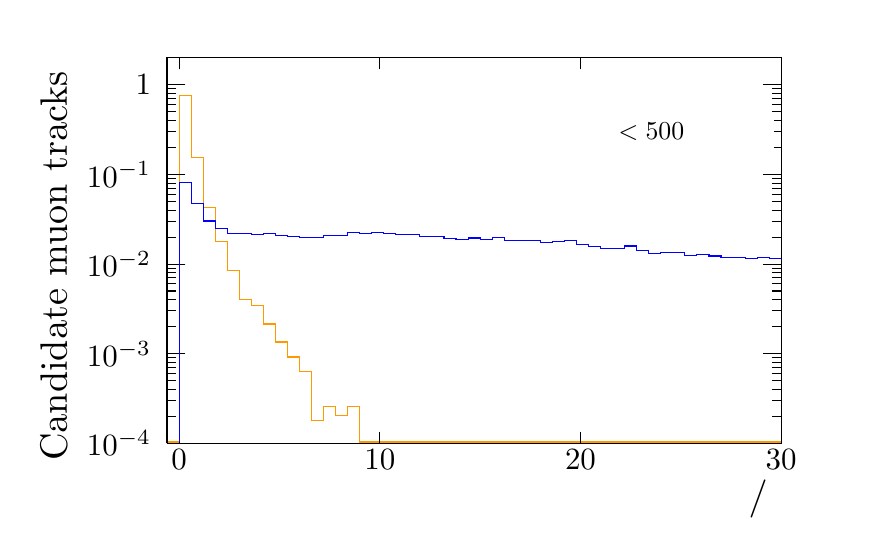
\begin{tikzpicture}
\pgfdeclareplotmark{cross} {
\pgfpathmoveto{\pgfpoint{-0.3\pgfplotmarksize}{\pgfplotmarksize}}
\pgfpathlineto{\pgfpoint{+0.3\pgfplotmarksize}{\pgfplotmarksize}}
\pgfpathlineto{\pgfpoint{+0.3\pgfplotmarksize}{0.3\pgfplotmarksize}}
\pgfpathlineto{\pgfpoint{+1\pgfplotmarksize}{0.3\pgfplotmarksize}}
\pgfpathlineto{\pgfpoint{+1\pgfplotmarksize}{-0.3\pgfplotmarksize}}
\pgfpathlineto{\pgfpoint{+0.3\pgfplotmarksize}{-0.3\pgfplotmarksize}}
\pgfpathlineto{\pgfpoint{+0.3\pgfplotmarksize}{-1.\pgfplotmarksize}}
\pgfpathlineto{\pgfpoint{-0.3\pgfplotmarksize}{-1.\pgfplotmarksize}}
\pgfpathlineto{\pgfpoint{-0.3\pgfplotmarksize}{-0.3\pgfplotmarksize}}
\pgfpathlineto{\pgfpoint{-1.\pgfplotmarksize}{-0.3\pgfplotmarksize}}
\pgfpathlineto{\pgfpoint{-1.\pgfplotmarksize}{0.3\pgfplotmarksize}}
\pgfpathlineto{\pgfpoint{-0.3\pgfplotmarksize}{0.3\pgfplotmarksize}}
\pgfpathclose
\pgfusepathqstroke
}
\pgfdeclareplotmark{cross*} {
\pgfpathmoveto{\pgfpoint{-0.3\pgfplotmarksize}{\pgfplotmarksize}}
\pgfpathlineto{\pgfpoint{+0.3\pgfplotmarksize}{\pgfplotmarksize}}
\pgfpathlineto{\pgfpoint{+0.3\pgfplotmarksize}{0.3\pgfplotmarksize}}
\pgfpathlineto{\pgfpoint{+1\pgfplotmarksize}{0.3\pgfplotmarksize}}
\pgfpathlineto{\pgfpoint{+1\pgfplotmarksize}{-0.3\pgfplotmarksize}}
\pgfpathlineto{\pgfpoint{+0.3\pgfplotmarksize}{-0.3\pgfplotmarksize}}
\pgfpathlineto{\pgfpoint{+0.3\pgfplotmarksize}{-1.\pgfplotmarksize}}
\pgfpathlineto{\pgfpoint{-0.3\pgfplotmarksize}{-1.\pgfplotmarksize}}
\pgfpathlineto{\pgfpoint{-0.3\pgfplotmarksize}{-0.3\pgfplotmarksize}}
\pgfpathlineto{\pgfpoint{-1.\pgfplotmarksize}{-0.3\pgfplotmarksize}}
\pgfpathlineto{\pgfpoint{-1.\pgfplotmarksize}{0.3\pgfplotmarksize}}
\pgfpathlineto{\pgfpoint{-0.3\pgfplotmarksize}{0.3\pgfplotmarksize}}
\pgfpathclose
\pgfusepathqfillstroke
}
\pgfdeclareplotmark{newstar} {
\pgfpathmoveto{\pgfqpoint{0pt}{\pgfplotmarksize}}
\pgfpathlineto{\pgfqpointpolar{44}{0.5\pgfplotmarksize}}
\pgfpathlineto{\pgfqpointpolar{18}{\pgfplotmarksize}}
\pgfpathlineto{\pgfqpointpolar{-20}{0.5\pgfplotmarksize}}
\pgfpathlineto{\pgfqpointpolar{-54}{\pgfplotmarksize}}
\pgfpathlineto{\pgfqpointpolar{-90}{0.5\pgfplotmarksize}}
\pgfpathlineto{\pgfqpointpolar{234}{\pgfplotmarksize}}
\pgfpathlineto{\pgfqpointpolar{198}{0.5\pgfplotmarksize}}
\pgfpathlineto{\pgfqpointpolar{162}{\pgfplotmarksize}}
\pgfpathlineto{\pgfqpointpolar{134}{0.5\pgfplotmarksize}}
\pgfpathclose
\pgfusepathqstroke
}
\pgfdeclareplotmark{newstar*} {
\pgfpathmoveto{\pgfqpoint{0pt}{\pgfplotmarksize}}
\pgfpathlineto{\pgfqpointpolar{44}{0.5\pgfplotmarksize}}
\pgfpathlineto{\pgfqpointpolar{18}{\pgfplotmarksize}}
\pgfpathlineto{\pgfqpointpolar{-20}{0.5\pgfplotmarksize}}
\pgfpathlineto{\pgfqpointpolar{-54}{\pgfplotmarksize}}
\pgfpathlineto{\pgfqpointpolar{-90}{0.5\pgfplotmarksize}}
\pgfpathlineto{\pgfqpointpolar{234}{\pgfplotmarksize}}
\pgfpathlineto{\pgfqpointpolar{198}{0.5\pgfplotmarksize}}
\pgfpathlineto{\pgfqpointpolar{162}{\pgfplotmarksize}}
\pgfpathlineto{\pgfqpointpolar{134}{0.5\pgfplotmarksize}}
\pgfpathclose
\pgfusepathqfillstroke
}
\definecolor{c}{rgb}{1,1,1};
\draw [color=c, fill=c] (0,0) rectangle (10,6.27517);
\draw [color=c, fill=c] (1.4,1.00403) rectangle (9.2,5.89866);
\definecolor{c}{rgb}{0,0,0};
\draw [c] (1.4,1.00403) -- (1.4,5.89866) -- (9.2,5.89866) -- (9.2,1.00403) -- (1.4,1.00403);
\definecolor{c}{rgb}{1,1,1};
\draw [color=c, fill=c] (1.4,1.00403) rectangle (9.2,5.89866);
\definecolor{c}{rgb}{0,0,0};
\draw [c] (1.4,1.00403) -- (1.4,5.89866) -- (9.2,5.89866) -- (9.2,1.00403) -- (1.4,1.00403);
\definecolor{c}{rgb}{1,0.6,0};
\draw [c,line width=0.4] (1.41678,1.02081) -- (1.41678,1.02081) -- (1.55294,1.02081) -- (1.55294,5.42255) -- (1.70588,5.42255) -- (1.70588,4.62973) -- (1.85882,4.62973) -- (1.85882,4.00033) -- (2.01176,4.00033) -- (2.01176,3.56618) --
 (2.16471,3.56618) -- (2.16471,3.20048) -- (2.31765,3.20048) -- (2.31765,2.83364) -- (2.47059,2.83364) -- (2.47059,2.75277) -- (2.62353,2.75277) -- (2.62353,2.51827) -- (2.77647,2.51827) -- (2.77647,2.29067) -- (2.92941,2.29067) -- (2.92941,2.09951)
 -- (3.08235,2.09951) -- (3.08235,1.91929) -- (3.23529,1.91929) -- (3.23529,1.29015) -- (3.38824,1.29015) -- (3.38824,1.46643) -- (3.54118,1.46643) -- (3.54118,1.35615) -- (3.69412,1.35615) -- (3.69412,1.46643) -- (3.84706,1.46643) --
 (3.84706,1.02081) -- (4,1.02081) -- (4,1.02081) -- (4.15294,1.02081) -- (4.15294,1.02081) -- (4.30588,1.02081) -- (4.30588,1.02081) -- (4.45882,1.02081) -- (4.45882,1.02081) -- (4.61176,1.02081) -- (4.61176,1.02081) -- (4.76471,1.02081) --
 (4.76471,1.02081) -- (4.91765,1.02081) -- (4.91765,1.02081) -- (5.07059,1.02081) -- (5.07059,1.02081) -- (5.22353,1.02081) -- (5.22353,1.02081) -- (5.37647,1.02081) -- (5.37647,1.02081) -- (5.52941,1.02081) -- (5.52941,1.02081) -- (5.68235,1.02081)
 -- (5.68235,1.02081) -- (5.83529,1.02081) -- (5.83529,1.02081) -- (5.98824,1.02081) -- (5.98824,1.02081) -- (6.14118,1.02081) -- (6.14118,1.02081) -- (6.29412,1.02081) -- (6.29412,1.02081) -- (6.44706,1.02081) -- (6.44706,1.02081) -- (6.6,1.02081)
 -- (6.6,1.02081) -- (6.75294,1.02081) -- (6.75294,1.02081) -- (6.90588,1.02081) -- (6.90588,1.02081) -- (7.05882,1.02081) -- (7.05882,1.02081) -- (7.21176,1.02081) -- (7.21176,1.02081) -- (7.36471,1.02081) -- (7.36471,1.02081) -- (7.51765,1.02081)
 -- (7.51765,1.02081) -- (7.67059,1.02081) -- (7.67059,1.02081) -- (7.82353,1.02081) -- (7.82353,1.02081) -- (7.97647,1.02081) -- (7.97647,1.02081) -- (8.12941,1.02081) -- (8.12941,1.02081) -- (8.28235,1.02081) -- (8.28235,1.02081) --
 (8.43529,1.02081) -- (8.43529,1.02081) -- (8.58823,1.02081) -- (8.58823,1.02081) -- (8.74118,1.02081) -- (8.74118,1.02081) -- (8.89412,1.02081) -- (8.89412,1.02081) -- (9.04706,1.02081) -- (9.04706,1.02081) -- (9.2,1.02081) -- (9.2,1.02081);
\definecolor{c}{rgb}{0,0,0};
\draw [c,line width=0.4] (1.4,1.00403) -- (9.2,1.00403);
\draw [anchor= east] (9.2,0.301208) node[scale=1.37879, rotate=0]{$\chisq/\nDoF$};
\draw [c,line width=0.4] (1.55294,1.15087) -- (1.55294,1.00403);
\draw [c,line width=0.4] (4.10196,1.15087) -- (4.10196,1.00403);
\draw [c,line width=0.4] (6.65098,1.15087) -- (6.65098,1.00403);
\draw [c,line width=0.4] (9.2,1.15087) -- (9.2,1.00403);
\draw [c,line width=0.4] (1.55294,1.15087) -- (1.55294,1.00403);
\draw [anchor=base] (1.55294,0.665168) node[scale=1.11794, rotate=0]{0};
\draw [anchor=base] (4.10196,0.665168) node[scale=1.11794, rotate=0]{10};
\draw [anchor=base] (6.65098,0.665168) node[scale=1.11794, rotate=0]{20};
\draw [anchor=base] (9.2,0.665168) node[scale=1.11794, rotate=0]{30};
\draw [c,line width=0.4] (1.4,5.89866) -- (9.2,5.89866);
\draw [c,line width=0.4] (1.55294,5.75182) -- (1.55294,5.89866);
\draw [c,line width=0.4] (4.10196,5.75182) -- (4.10196,5.89866);
\draw [c,line width=0.4] (6.65098,5.75182) -- (6.65098,5.89866);
\draw [c,line width=0.4] (9.2,5.75182) -- (9.2,5.89866);
\draw [c,line width=0.4] (1.55294,5.75182) -- (1.55294,5.89866);
\draw [c,line width=0.4] (1.4,1.00403) -- (1.4,5.89866);
\draw [anchor= east] (-0.04,5.89866) node[scale=1.37879, rotate=90]{Candidate muon tracks};
\draw [c,line width=0.4] (1.634,1.00403) -- (1.4,1.00403);
\draw [anchor= east] (1.336,1.00403) node[scale=1.11794, rotate=0]{$10^{-4}$};
\draw [c,line width=0.4] (1.517,1.3466) -- (1.4,1.3466);
\draw [c,line width=0.4] (1.517,1.547) -- (1.4,1.547);
\draw [c,line width=0.4] (1.517,1.68918) -- (1.4,1.68918);
\draw [c,line width=0.4] (1.517,1.79947) -- (1.4,1.79947);
\draw [c,line width=0.4] (1.517,1.88957) -- (1.4,1.88957);
\draw [c,line width=0.4] (1.517,1.96576) -- (1.4,1.96576);
\draw [c,line width=0.4] (1.517,2.03176) -- (1.4,2.03176);
\draw [c,line width=0.4] (1.517,2.08997) -- (1.4,2.08997);
\draw [c,line width=0.4] (1.634,2.14204) -- (1.4,2.14204);
\draw [anchor= east] (1.336,2.14204) node[scale=1.11794, rotate=0]{$10^{-3}$};
\draw [c,line width=0.4] (1.517,2.48462) -- (1.4,2.48462);
\draw [c,line width=0.4] (1.517,2.68501) -- (1.4,2.68501);
\draw [c,line width=0.4] (1.517,2.82719) -- (1.4,2.82719);
\draw [c,line width=0.4] (1.517,2.93748) -- (1.4,2.93748);
\draw [c,line width=0.4] (1.517,3.02759) -- (1.4,3.02759);
\draw [c,line width=0.4] (1.517,3.10377) -- (1.4,3.10377);
\draw [c,line width=0.4] (1.517,3.16977) -- (1.4,3.16977);
\draw [c,line width=0.4] (1.517,3.22798) -- (1.4,3.22798);
\draw [c,line width=0.4] (1.634,3.28005) -- (1.4,3.28005);
\draw [anchor= east] (1.336,3.28005) node[scale=1.11794, rotate=0]{$10^{-2}$};
\draw [c,line width=0.4] (1.517,3.62263) -- (1.4,3.62263);
\draw [c,line width=0.4] (1.517,3.82303) -- (1.4,3.82303);
\draw [c,line width=0.4] (1.517,3.96521) -- (1.4,3.96521);
\draw [c,line width=0.4] (1.517,4.07549) -- (1.4,4.07549);
\draw [c,line width=0.4] (1.517,4.1656) -- (1.4,4.1656);
\draw [c,line width=0.4] (1.517,4.24179) -- (1.4,4.24179);
\draw [c,line width=0.4] (1.517,4.30778) -- (1.4,4.30778);
\draw [c,line width=0.4] (1.517,4.366) -- (1.4,4.366);
\draw [c,line width=0.4] (1.634,4.41807) -- (1.4,4.41807);
\draw [anchor= east] (1.336,4.41807) node[scale=1.11794, rotate=0]{$10^{-1}$};
\draw [c,line width=0.4] (1.517,4.76064) -- (1.4,4.76064);
\draw [c,line width=0.4] (1.517,4.96104) -- (1.4,4.96104);
\draw [c,line width=0.4] (1.517,5.10322) -- (1.4,5.10322);
\draw [c,line width=0.4] (1.517,5.21351) -- (1.4,5.21351);
\draw [c,line width=0.4] (1.517,5.30361) -- (1.4,5.30361);
\draw [c,line width=0.4] (1.517,5.3798) -- (1.4,5.3798);
\draw [c,line width=0.4] (1.517,5.4458) -- (1.4,5.4458);
\draw [c,line width=0.4] (1.517,5.50401) -- (1.4,5.50401);
\draw [c,line width=0.4] (1.634,5.55608) -- (1.4,5.55608);
\draw [anchor= east] (1.336,5.55608) node[scale=1.11794, rotate=0]{1};
\draw [c,line width=0.4] (1.517,5.89866) -- (1.4,5.89866);
\draw [c,line width=0.4] (9.2,1.00403) -- (9.2,5.89866);
\draw [c,line width=0.4] (8.966,1.00403) -- (9.2,1.00403);
\draw [c,line width=0.4] (9.083,1.3466) -- (9.2,1.3466);
\draw [c,line width=0.4] (9.083,1.547) -- (9.2,1.547);
\draw [c,line width=0.4] (9.083,1.68918) -- (9.2,1.68918);
\draw [c,line width=0.4] (9.083,1.79947) -- (9.2,1.79947);
\draw [c,line width=0.4] (9.083,1.88957) -- (9.2,1.88957);
\draw [c,line width=0.4] (9.083,1.96576) -- (9.2,1.96576);
\draw [c,line width=0.4] (9.083,2.03176) -- (9.2,2.03176);
\draw [c,line width=0.4] (9.083,2.08997) -- (9.2,2.08997);
\draw [c,line width=0.4] (8.966,2.14204) -- (9.2,2.14204);
\draw [c,line width=0.4] (9.083,2.48462) -- (9.2,2.48462);
\draw [c,line width=0.4] (9.083,2.68501) -- (9.2,2.68501);
\draw [c,line width=0.4] (9.083,2.82719) -- (9.2,2.82719);
\draw [c,line width=0.4] (9.083,2.93748) -- (9.2,2.93748);
\draw [c,line width=0.4] (9.083,3.02759) -- (9.2,3.02759);
\draw [c,line width=0.4] (9.083,3.10377) -- (9.2,3.10377);
\draw [c,line width=0.4] (9.083,3.16977) -- (9.2,3.16977);
\draw [c,line width=0.4] (9.083,3.22798) -- (9.2,3.22798);
\draw [c,line width=0.4] (8.966,3.28005) -- (9.2,3.28005);
\draw [c,line width=0.4] (9.083,3.62263) -- (9.2,3.62263);
\draw [c,line width=0.4] (9.083,3.82303) -- (9.2,3.82303);
\draw [c,line width=0.4] (9.083,3.96521) -- (9.2,3.96521);
\draw [c,line width=0.4] (9.083,4.07549) -- (9.2,4.07549);
\draw [c,line width=0.4] (9.083,4.1656) -- (9.2,4.1656);
\draw [c,line width=0.4] (9.083,4.24179) -- (9.2,4.24179);
\draw [c,line width=0.4] (9.083,4.30778) -- (9.2,4.30778);
\draw [c,line width=0.4] (9.083,4.366) -- (9.2,4.366);
\draw [c,line width=0.4] (8.966,4.41807) -- (9.2,4.41807);
\draw [c,line width=0.4] (9.083,4.76064) -- (9.2,4.76064);
\draw [c,line width=0.4] (9.083,4.96104) -- (9.2,4.96104);
\draw [c,line width=0.4] (9.083,5.10322) -- (9.2,5.10322);
\draw [c,line width=0.4] (9.083,5.21351) -- (9.2,5.21351);
\draw [c,line width=0.4] (9.083,5.30361) -- (9.2,5.30361);
\draw [c,line width=0.4] (9.083,5.3798) -- (9.2,5.3798);
\draw [c,line width=0.4] (9.083,5.4458) -- (9.2,5.4458);
\draw [c,line width=0.4] (9.083,5.50401) -- (9.2,5.50401);
\draw [c,line width=0.4] (8.966,5.55608) -- (9.2,5.55608);
\draw [c,line width=0.4] (9.083,5.89866) -- (9.2,5.89866);
\definecolor{c}{rgb}{0,0,1};
\draw [c,line width=0.4] (1.55294,1.02081) -- (1.55294,4.31946) -- (1.70588,4.31946) -- (1.70588,4.04993) -- (1.85882,4.04993) -- (1.85882,3.82753) -- (2.01176,3.82753) -- (2.01176,3.73489) -- (2.16471,3.73489) -- (2.16471,3.6723) -- (2.31765,3.6723)
 -- (2.31765,3.66634) -- (2.47059,3.66634) -- (2.47059,3.65572) -- (2.62353,3.65572) -- (2.62353,3.66634) -- (2.77647,3.66634) -- (2.77647,3.64067) -- (2.92941,3.64067) -- (2.92941,3.63056) -- (3.08235,3.63056) -- (3.08235,3.61748) --
 (3.23529,3.61748) -- (3.23529,3.61526) -- (3.38824,3.61526) -- (3.38824,3.64434) -- (3.54118,3.64434) -- (3.54118,3.64747) -- (3.69412,3.64747) -- (3.69412,3.68451) -- (3.84706,3.68451) -- (3.84706,3.6723) -- (4,3.6723) -- (4,3.68451) --
 (4.15294,3.68451) -- (4.15294,3.6723) -- (4.30588,3.6723) -- (4.30588,3.65979) -- (4.45882,3.65979) -- (4.45882,3.65006) -- (4.61176,3.65006) -- (4.61176,3.62569) -- (4.76471,3.62569) -- (4.76471,3.62948) -- (4.91765,3.62948) -- (4.91765,3.60631) --
 (5.07059,3.60631) -- (5.07059,3.5943) -- (5.22353,3.5943) -- (5.22353,3.61137) -- (5.37647,3.61137) -- (5.37647,3.58789) -- (5.52941,3.58789) -- (5.52941,3.61526) -- (5.68235,3.61526) -- (5.68235,3.5814) -- (5.83529,3.5814) -- (5.83529,3.5814) --
 (5.98824,3.5814) -- (5.98824,3.57783) -- (6.14118,3.57783) -- (6.14118,3.55014) -- (6.29412,3.55014) -- (6.29412,3.56816) -- (6.44706,3.56816) -- (6.44706,3.57723) -- (6.6,3.57723) -- (6.6,3.53078) -- (6.75294,3.53078) -- (6.75294,3.50788) --
 (6.90588,3.50788) -- (6.90588,3.47732) -- (7.05882,3.47732) -- (7.05882,3.48024) -- (7.21176,3.48024) -- (7.21176,3.50926) -- (7.36471,3.50926) -- (7.36471,3.45251) -- (7.51765,3.45251) -- (7.51765,3.41404) -- (7.67059,3.41404) -- (7.67059,3.42882)
 -- (7.82353,3.42882) -- (7.82353,3.42312) -- (7.97647,3.42312) -- (7.97647,3.38397) -- (8.12941,3.38397) -- (8.12941,3.3988) -- (8.28235,3.3988) -- (8.28235,3.3822) -- (8.43529,3.3822) -- (8.43529,3.36132) -- (8.58823,3.36132) -- (8.58823,3.36317)
 -- (8.74118,3.36317) -- (8.74118,3.35195) -- (8.89412,3.35195) -- (8.89412,3.36501) -- (9.04706,3.36501) -- (9.04706,3.3453) -- (9.2,3.3453);
\definecolor{c}{rgb}{1,1,1};
\draw [color=c, fill=c] (6,4.70638) rectangle (9.1,5.20839);
\draw (7.55,4.95738) node[scale=0.931615, rotate=0]{$\pt < 500 \mevc$};
\end{tikzpicture}
}
    \caption{}
    \label{mvm_chi2}
  \end{subfigure}
  \caption{Distribution of the \chisq variable between the old (left) and the new (right) matching algorithms.
           Only low momentum muon tracks are considered. Matched (not matched) muon tracks are shown with orange (blue).}
 \label{mvm_chi2_comp}
\end{figure}

\subsubsection{z focal plane parametrization}
The empirical parametrization of the magnet focal plane $z$ coordinate already used in the old \mvm \cite{roelThesis},
is updated. Furthermore the uncertainties on the focal plane intersection estimate are empirically estimated using simulated data.
Specifically, since the true muon track is known it is possible to tune these uncertainties such that they yield the same momentum
estimation as the full computation of the muon trajectory would do. Note that a momentum estimate is available by the
\mvTTm algorithm as soon as a seed hit in M3 is found, using the kick method.

\begin{figure}[t]
  \centering
  \begin{subfigure}{0.5\textwidth}
    \raggedright
    \tikzsetnextfilename{mvTTm_wind_eff_total_x}
    \scalebox{.55}{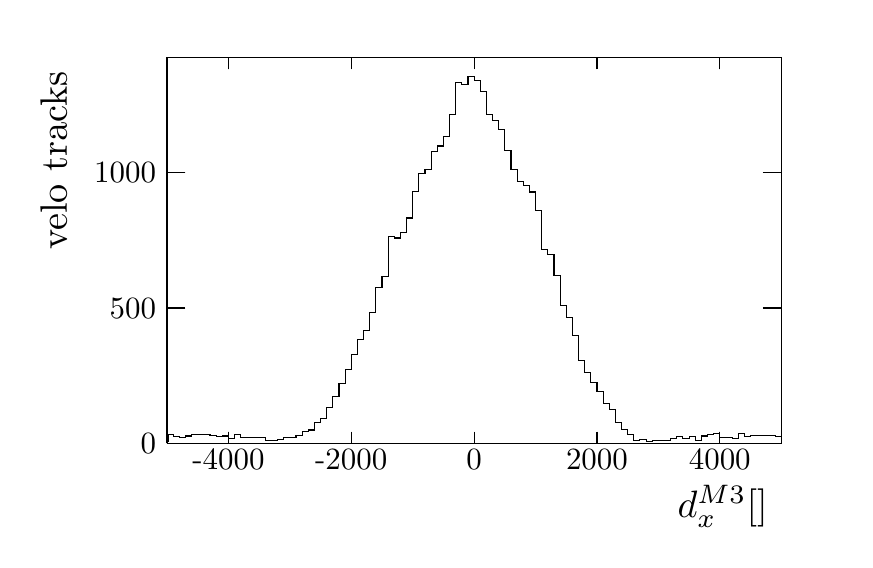
\begin{tikzpicture}
\pgfdeclareplotmark{cross} {
\pgfpathmoveto{\pgfpoint{-0.3\pgfplotmarksize}{\pgfplotmarksize}}
\pgfpathlineto{\pgfpoint{+0.3\pgfplotmarksize}{\pgfplotmarksize}}
\pgfpathlineto{\pgfpoint{+0.3\pgfplotmarksize}{0.3\pgfplotmarksize}}
\pgfpathlineto{\pgfpoint{+1\pgfplotmarksize}{0.3\pgfplotmarksize}}
\pgfpathlineto{\pgfpoint{+1\pgfplotmarksize}{-0.3\pgfplotmarksize}}
\pgfpathlineto{\pgfpoint{+0.3\pgfplotmarksize}{-0.3\pgfplotmarksize}}
\pgfpathlineto{\pgfpoint{+0.3\pgfplotmarksize}{-1.\pgfplotmarksize}}
\pgfpathlineto{\pgfpoint{-0.3\pgfplotmarksize}{-1.\pgfplotmarksize}}
\pgfpathlineto{\pgfpoint{-0.3\pgfplotmarksize}{-0.3\pgfplotmarksize}}
\pgfpathlineto{\pgfpoint{-1.\pgfplotmarksize}{-0.3\pgfplotmarksize}}
\pgfpathlineto{\pgfpoint{-1.\pgfplotmarksize}{0.3\pgfplotmarksize}}
\pgfpathlineto{\pgfpoint{-0.3\pgfplotmarksize}{0.3\pgfplotmarksize}}
\pgfpathclose
\pgfusepathqstroke
}
\pgfdeclareplotmark{cross*} {
\pgfpathmoveto{\pgfpoint{-0.3\pgfplotmarksize}{\pgfplotmarksize}}
\pgfpathlineto{\pgfpoint{+0.3\pgfplotmarksize}{\pgfplotmarksize}}
\pgfpathlineto{\pgfpoint{+0.3\pgfplotmarksize}{0.3\pgfplotmarksize}}
\pgfpathlineto{\pgfpoint{+1\pgfplotmarksize}{0.3\pgfplotmarksize}}
\pgfpathlineto{\pgfpoint{+1\pgfplotmarksize}{-0.3\pgfplotmarksize}}
\pgfpathlineto{\pgfpoint{+0.3\pgfplotmarksize}{-0.3\pgfplotmarksize}}
\pgfpathlineto{\pgfpoint{+0.3\pgfplotmarksize}{-1.\pgfplotmarksize}}
\pgfpathlineto{\pgfpoint{-0.3\pgfplotmarksize}{-1.\pgfplotmarksize}}
\pgfpathlineto{\pgfpoint{-0.3\pgfplotmarksize}{-0.3\pgfplotmarksize}}
\pgfpathlineto{\pgfpoint{-1.\pgfplotmarksize}{-0.3\pgfplotmarksize}}
\pgfpathlineto{\pgfpoint{-1.\pgfplotmarksize}{0.3\pgfplotmarksize}}
\pgfpathlineto{\pgfpoint{-0.3\pgfplotmarksize}{0.3\pgfplotmarksize}}
\pgfpathclose
\pgfusepathqfillstroke
}
\pgfdeclareplotmark{newstar} {
\pgfpathmoveto{\pgfqpoint{0pt}{\pgfplotmarksize}}
\pgfpathlineto{\pgfqpointpolar{44}{0.5\pgfplotmarksize}}
\pgfpathlineto{\pgfqpointpolar{18}{\pgfplotmarksize}}
\pgfpathlineto{\pgfqpointpolar{-20}{0.5\pgfplotmarksize}}
\pgfpathlineto{\pgfqpointpolar{-54}{\pgfplotmarksize}}
\pgfpathlineto{\pgfqpointpolar{-90}{0.5\pgfplotmarksize}}
\pgfpathlineto{\pgfqpointpolar{234}{\pgfplotmarksize}}
\pgfpathlineto{\pgfqpointpolar{198}{0.5\pgfplotmarksize}}
\pgfpathlineto{\pgfqpointpolar{162}{\pgfplotmarksize}}
\pgfpathlineto{\pgfqpointpolar{134}{0.5\pgfplotmarksize}}
\pgfpathclose
\pgfusepathqstroke
}
\pgfdeclareplotmark{newstar*} {
\pgfpathmoveto{\pgfqpoint{0pt}{\pgfplotmarksize}}
\pgfpathlineto{\pgfqpointpolar{44}{0.5\pgfplotmarksize}}
\pgfpathlineto{\pgfqpointpolar{18}{\pgfplotmarksize}}
\pgfpathlineto{\pgfqpointpolar{-20}{0.5\pgfplotmarksize}}
\pgfpathlineto{\pgfqpointpolar{-54}{\pgfplotmarksize}}
\pgfpathlineto{\pgfqpointpolar{-90}{0.5\pgfplotmarksize}}
\pgfpathlineto{\pgfqpointpolar{234}{\pgfplotmarksize}}
\pgfpathlineto{\pgfqpointpolar{198}{0.5\pgfplotmarksize}}
\pgfpathlineto{\pgfqpointpolar{162}{\pgfplotmarksize}}
\pgfpathlineto{\pgfqpointpolar{134}{0.5\pgfplotmarksize}}
\pgfpathclose
\pgfusepathqfillstroke
}
\definecolor{c}{rgb}{1,1,1};
\draw [color=c, fill=c] (0,0) rectangle (10,6.27517);
\draw [color=c, fill=c] (1.4,1.00403) rectangle (9.2,5.89866);
\definecolor{c}{rgb}{0,0,0};
\draw [c] (1.4,1.00403) -- (1.4,5.89866) -- (9.2,5.89866) -- (9.2,1.00403) -- (1.4,1.00403);
\definecolor{c}{rgb}{1,1,1};
\draw [color=c, fill=c] (1.4,1.00403) rectangle (9.2,5.89866);
\definecolor{c}{rgb}{0,0,0};
\draw [c] (1.4,1.00403) -- (1.4,5.89866) -- (9.2,5.89866) -- (9.2,1.00403) -- (1.4,1.00403);
\draw [c,line width=0.4] (1.41678,1.02081) -- (1.41678,1.12082) -- (1.478,1.12082) -- (1.478,1.08647) -- (1.556,1.08647) -- (1.556,1.07617) -- (1.634,1.07617) -- (1.634,1.09678) -- (1.712,1.09678) -- (1.712,1.11395) -- (1.79,1.11395) --
 (1.79,1.11739) -- (1.868,1.11739) -- (1.868,1.11395) -- (1.946,1.11395) -- (1.946,1.10708) -- (2.024,1.10708) -- (2.024,1.09334) -- (2.102,1.09334) -- (2.102,1.09678) -- (2.18,1.09678) -- (2.18,1.0693) -- (2.258,1.0693) -- (2.258,1.11052) --
 (2.336,1.11052) -- (2.336,1.07273) -- (2.414,1.07273) -- (2.414,1.08304) -- (2.492,1.08304) -- (2.492,1.07617) -- (2.57,1.07617) -- (2.57,1.07273) -- (2.648,1.07273) -- (2.648,1.03838) -- (2.726,1.03838) -- (2.726,1.03494) -- (2.804,1.03494) --
 (2.804,1.04868) -- (2.882,1.04868) -- (2.882,1.08304) -- (2.96,1.08304) -- (2.96,1.07617) -- (3.038,1.07617) -- (3.038,1.10708) -- (3.116,1.10708) -- (3.116,1.1483) -- (3.194,1.1483) -- (3.194,1.17235) -- (3.272,1.17235) -- (3.272,1.27197) --
 (3.35,1.27197) -- (3.35,1.31663) -- (3.428,1.31663) -- (3.428,1.45404) -- (3.506,1.45404) -- (3.506,1.59831) -- (3.584,1.59831) -- (3.584,1.76664) -- (3.662,1.76664) -- (3.662,1.94183) -- (3.74,1.94183) -- (3.74,2.1342) -- (3.818,2.1342) --
 (3.818,2.32314) -- (3.896,2.32314) -- (3.896,2.43307) -- (3.974,2.43307) -- (3.974,2.67009) -- (4.052,2.67009) -- (4.052,2.9827) -- (4.13,2.9827) -- (4.13,3.11667) -- (4.208,3.11667) -- (4.208,3.63195) -- (4.286,3.63195) -- (4.286,3.61134) --
 (4.364,3.61134) -- (4.364,3.6766) -- (4.442,3.6766) -- (4.442,3.86554) -- (4.52,3.86554) -- (4.52,4.20562) -- (4.598,4.20562) -- (4.598,4.42891) -- (4.676,4.42891) -- (4.676,4.477) -- (4.754,4.477) -- (4.754,4.7106) -- (4.832,4.7106) --
 (4.832,4.7793) -- (4.91,4.7793) -- (4.91,4.8961) -- (4.988,4.8961) -- (4.988,5.18465) -- (5.066,5.18465) -- (5.066,5.58314) -- (5.144,5.58314) -- (5.144,5.55565) -- (5.222,5.55565) -- (5.222,5.66558) -- (5.3,5.66558) -- (5.3,5.60718) --
 (5.378,5.60718) -- (5.378,5.46977) -- (5.456,5.46977) -- (5.456,5.18465) -- (5.534,5.18465) -- (5.534,5.10221) -- (5.612,5.10221) -- (5.612,4.99228) -- (5.69,4.99228) -- (5.69,4.72777) -- (5.768,4.72777) -- (5.768,4.477) -- (5.846,4.477) --
 (5.846,4.32929) -- (5.924,4.32929) -- (5.924,4.27776) -- (6.002,4.27776) -- (6.002,4.19532) -- (6.08,4.19532) -- (6.08,3.96173) -- (6.158,3.96173) -- (6.158,3.46706) -- (6.236,3.46706) -- (6.236,3.40179) -- (6.314,3.40179) -- (6.314,3.13041) --
 (6.392,3.13041) -- (6.392,2.75254) -- (6.47,2.75254) -- (6.47,2.60139) -- (6.548,2.60139) -- (6.548,2.3781) -- (6.626,2.3781) -- (6.626,2.05176) -- (6.704,2.05176) -- (6.704,1.90405) -- (6.782,1.90405) -- (6.782,1.77351) -- (6.86,1.77351) --
 (6.86,1.66358) -- (6.938,1.66358) -- (6.938,1.50556) -- (7.016,1.50556) -- (7.016,1.43686) -- (7.094,1.43686) -- (7.094,1.27197) -- (7.172,1.27197) -- (7.172,1.18266) -- (7.25,1.18266) -- (7.25,1.11395) -- (7.328,1.11395) -- (7.328,1.03838) --
 (7.406,1.03838) -- (7.406,1.04868) -- (7.484,1.04868) -- (7.484,1.0212) -- (7.562,1.0212) -- (7.562,1.04181) -- (7.64,1.04181) -- (7.64,1.03494) -- (7.718,1.03494) -- (7.718,1.03838) -- (7.796,1.03838) -- (7.796,1.06243) -- (7.874,1.06243) --
 (7.874,1.08647) -- (7.952,1.08647) -- (7.952,1.0693) -- (8.03,1.0693) -- (8.03,1.08647) -- (8.108,1.08647) -- (8.108,1.03494) -- (8.186,1.03494) -- (8.186,1.09678) -- (8.264,1.09678) -- (8.264,1.11395) -- (8.342,1.11395) -- (8.342,1.12769) --
 (8.42,1.12769) -- (8.42,1.08304) -- (8.498,1.08304) -- (8.498,1.07273) -- (8.576,1.07273) -- (8.576,1.06586) -- (8.654,1.06586) -- (8.654,1.12769) -- (8.732,1.12769) -- (8.732,1.08991) -- (8.81,1.08991) -- (8.81,1.10365) -- (8.888,1.10365) --
 (8.888,1.10365) -- (8.966,1.10365) -- (8.966,1.10021) -- (9.044,1.10021) -- (9.044,1.10365) -- (9.122,1.10365) -- (9.122,1.09334) -- (9.2,1.09334);
\draw [c,line width=0.4] (1.4,1.00403) -- (9.2,1.00403);
\draw [anchor= east] (9.2,0.200805) node[scale=1.37879, rotate=0]{$d^{\text{M3}}_x [\mm]$};
\draw [c,line width=0.4] (2.18,1.15087) -- (2.18,1.00403);
\draw [c,line width=0.4] (3.74,1.15087) -- (3.74,1.00403);
\draw [c,line width=0.4] (5.3,1.15087) -- (5.3,1.00403);
\draw [c,line width=0.4] (6.86,1.15087) -- (6.86,1.00403);
\draw [c,line width=0.4] (8.42,1.15087) -- (8.42,1.00403);
\draw [c,line width=0.4] (2.18,1.15087) -- (2.18,1.00403);
\draw [c,line width=0.4] (8.42,1.15087) -- (8.42,1.00403);
\draw [anchor=base] (2.18,0.665168) node[scale=1.11794, rotate=0]{-4000};
\draw [anchor=base] (3.74,0.665168) node[scale=1.11794, rotate=0]{-2000};
\draw [anchor=base] (5.3,0.665168) node[scale=1.11794, rotate=0]{0};
\draw [anchor=base] (6.86,0.665168) node[scale=1.11794, rotate=0]{2000};
\draw [anchor=base] (8.42,0.665168) node[scale=1.11794, rotate=0]{4000};
\draw [c,line width=0.4] (1.4,5.89866) -- (9.2,5.89866);
\draw [c,line width=0.4] (2.18,5.75182) -- (2.18,5.89866);
\draw [c,line width=0.4] (3.74,5.75182) -- (3.74,5.89866);
\draw [c,line width=0.4] (5.3,5.75182) -- (5.3,5.89866);
\draw [c,line width=0.4] (6.86,5.75182) -- (6.86,5.89866);
\draw [c,line width=0.4] (8.42,5.75182) -- (8.42,5.89866);
\draw [c,line width=0.4] (2.18,5.75182) -- (2.18,5.89866);
\draw [c,line width=0.4] (8.42,5.75182) -- (8.42,5.89866);
\draw [c,line width=0.4] (1.4,1.00403) -- (1.4,5.89866);
\draw [anchor= east] (-0.04,5.89866) node[scale=1.37879, rotate=90]{velo tracks};
\draw [c,line width=0.4] (1.634,1.00403) -- (1.4,1.00403);
\draw [c,line width=0.4] (1.634,2.72162) -- (1.4,2.72162);
\draw [c,line width=0.4] (1.634,4.43922) -- (1.4,4.43922);
\draw [c,line width=0.4] (1.634,4.43922) -- (1.4,4.43922);
\draw [anchor= east] (1.4,1.00403) node[scale=1.11794, rotate=0]{0};
\draw [anchor= east] (1.4,2.72162) node[scale=1.11794, rotate=0]{500};
\draw [anchor= east] (1.4,4.43922) node[scale=1.11794, rotate=0]{1000};
\draw [c,line width=0.4] (9.2,1.00403) -- (9.2,5.89866);
\draw [c,line width=0.4] (8.966,1.00403) -- (9.2,1.00403);
\draw [c,line width=0.4] (8.966,2.72162) -- (9.2,2.72162);
\draw [c,line width=0.4] (8.966,4.43922) -- (9.2,4.43922);
\draw [c,line width=0.4] (8.966,4.43922) -- (9.2,4.43922);
\end{tikzpicture}
}
    \caption{}
    \label{mvTTm_res_x}
  \end{subfigure}%
  \hfill%
  \begin{subfigure}{0.5\textwidth}
    \raggedleft
    \tikzsetnextfilename{mvTTm_wind_eff_total_y}
    \scalebox{.55}{\begin{tikzpicture}
\pgfdeclareplotmark{cross} {
\pgfpathmoveto{\pgfpoint{-0.3\pgfplotmarksize}{\pgfplotmarksize}}
\pgfpathlineto{\pgfpoint{+0.3\pgfplotmarksize}{\pgfplotmarksize}}
\pgfpathlineto{\pgfpoint{+0.3\pgfplotmarksize}{0.3\pgfplotmarksize}}
\pgfpathlineto{\pgfpoint{+1\pgfplotmarksize}{0.3\pgfplotmarksize}}
\pgfpathlineto{\pgfpoint{+1\pgfplotmarksize}{-0.3\pgfplotmarksize}}
\pgfpathlineto{\pgfpoint{+0.3\pgfplotmarksize}{-0.3\pgfplotmarksize}}
\pgfpathlineto{\pgfpoint{+0.3\pgfplotmarksize}{-1.\pgfplotmarksize}}
\pgfpathlineto{\pgfpoint{-0.3\pgfplotmarksize}{-1.\pgfplotmarksize}}
\pgfpathlineto{\pgfpoint{-0.3\pgfplotmarksize}{-0.3\pgfplotmarksize}}
\pgfpathlineto{\pgfpoint{-1.\pgfplotmarksize}{-0.3\pgfplotmarksize}}
\pgfpathlineto{\pgfpoint{-1.\pgfplotmarksize}{0.3\pgfplotmarksize}}
\pgfpathlineto{\pgfpoint{-0.3\pgfplotmarksize}{0.3\pgfplotmarksize}}
\pgfpathclose
\pgfusepathqstroke
}
\pgfdeclareplotmark{cross*} {
\pgfpathmoveto{\pgfpoint{-0.3\pgfplotmarksize}{\pgfplotmarksize}}
\pgfpathlineto{\pgfpoint{+0.3\pgfplotmarksize}{\pgfplotmarksize}}
\pgfpathlineto{\pgfpoint{+0.3\pgfplotmarksize}{0.3\pgfplotmarksize}}
\pgfpathlineto{\pgfpoint{+1\pgfplotmarksize}{0.3\pgfplotmarksize}}
\pgfpathlineto{\pgfpoint{+1\pgfplotmarksize}{-0.3\pgfplotmarksize}}
\pgfpathlineto{\pgfpoint{+0.3\pgfplotmarksize}{-0.3\pgfplotmarksize}}
\pgfpathlineto{\pgfpoint{+0.3\pgfplotmarksize}{-1.\pgfplotmarksize}}
\pgfpathlineto{\pgfpoint{-0.3\pgfplotmarksize}{-1.\pgfplotmarksize}}
\pgfpathlineto{\pgfpoint{-0.3\pgfplotmarksize}{-0.3\pgfplotmarksize}}
\pgfpathlineto{\pgfpoint{-1.\pgfplotmarksize}{-0.3\pgfplotmarksize}}
\pgfpathlineto{\pgfpoint{-1.\pgfplotmarksize}{0.3\pgfplotmarksize}}
\pgfpathlineto{\pgfpoint{-0.3\pgfplotmarksize}{0.3\pgfplotmarksize}}
\pgfpathclose
\pgfusepathqfillstroke
}
\pgfdeclareplotmark{newstar} {
\pgfpathmoveto{\pgfqpoint{0pt}{\pgfplotmarksize}}
\pgfpathlineto{\pgfqpointpolar{44}{0.5\pgfplotmarksize}}
\pgfpathlineto{\pgfqpointpolar{18}{\pgfplotmarksize}}
\pgfpathlineto{\pgfqpointpolar{-20}{0.5\pgfplotmarksize}}
\pgfpathlineto{\pgfqpointpolar{-54}{\pgfplotmarksize}}
\pgfpathlineto{\pgfqpointpolar{-90}{0.5\pgfplotmarksize}}
\pgfpathlineto{\pgfqpointpolar{234}{\pgfplotmarksize}}
\pgfpathlineto{\pgfqpointpolar{198}{0.5\pgfplotmarksize}}
\pgfpathlineto{\pgfqpointpolar{162}{\pgfplotmarksize}}
\pgfpathlineto{\pgfqpointpolar{134}{0.5\pgfplotmarksize}}
\pgfpathclose
\pgfusepathqstroke
}
\pgfdeclareplotmark{newstar*} {
\pgfpathmoveto{\pgfqpoint{0pt}{\pgfplotmarksize}}
\pgfpathlineto{\pgfqpointpolar{44}{0.5\pgfplotmarksize}}
\pgfpathlineto{\pgfqpointpolar{18}{\pgfplotmarksize}}
\pgfpathlineto{\pgfqpointpolar{-20}{0.5\pgfplotmarksize}}
\pgfpathlineto{\pgfqpointpolar{-54}{\pgfplotmarksize}}
\pgfpathlineto{\pgfqpointpolar{-90}{0.5\pgfplotmarksize}}
\pgfpathlineto{\pgfqpointpolar{234}{\pgfplotmarksize}}
\pgfpathlineto{\pgfqpointpolar{198}{0.5\pgfplotmarksize}}
\pgfpathlineto{\pgfqpointpolar{162}{\pgfplotmarksize}}
\pgfpathlineto{\pgfqpointpolar{134}{0.5\pgfplotmarksize}}
\pgfpathclose
\pgfusepathqfillstroke
}
\definecolor{c}{rgb}{1,1,1};
\draw [color=c, fill=c] (0,0) rectangle (10,6.27517);
\draw [color=c, fill=c] (1.4,1.00403) rectangle (9.2,5.89866);
\definecolor{c}{rgb}{0,0,0};
\draw [c] (1.4,1.00403) -- (1.4,5.89866) -- (9.2,5.89866) -- (9.2,1.00403) -- (1.4,1.00403);
\definecolor{c}{rgb}{1,1,1};
\draw [color=c, fill=c] (1.4,1.00403) rectangle (9.2,5.89866);
\definecolor{c}{rgb}{0,0,0};
\draw [c] (1.4,1.00403) -- (1.4,5.89866) -- (9.2,5.89866) -- (9.2,1.00403) -- (1.4,1.00403);
\draw [c,line width=0.4] (1.41678,1.02081) -- (1.41678,1.02081) -- (1.478,1.02081) -- (1.478,1.02081) -- (1.556,1.02081) -- (1.556,1.02081) -- (1.634,1.02081) -- (1.634,1.02081) -- (1.712,1.02081) -- (1.712,1.02081) -- (1.79,1.02081) --
 (1.79,1.02081) -- (1.868,1.02081) -- (1.868,1.02081) -- (1.946,1.02081) -- (1.946,1.02081) -- (2.024,1.02081) -- (2.024,1.02081) -- (2.102,1.02081) -- (2.102,1.02081) -- (2.18,1.02081) -- (2.18,1.02081) -- (2.258,1.02081) -- (2.258,1.02081) --
 (2.336,1.02081) -- (2.336,1.02081) -- (2.414,1.02081) -- (2.414,1.02081) -- (2.492,1.02081) -- (2.492,1.02081) -- (2.57,1.02081) -- (2.57,1.02081) -- (2.648,1.02081) -- (2.648,1.02081) -- (2.726,1.02081) -- (2.726,1.02081) -- (2.804,1.02081) --
 (2.804,1.02081) -- (2.882,1.02081) -- (2.882,1.02081) -- (2.96,1.02081) -- (2.96,1.02081) -- (3.038,1.02081) -- (3.038,1.02081) -- (3.116,1.02081) -- (3.116,1.02081) -- (3.194,1.02081) -- (3.194,1.02081) -- (3.272,1.02081) -- (3.272,1.02081) --
 (3.35,1.02081) -- (3.35,1.02081) -- (3.428,1.02081) -- (3.428,1.02081) -- (3.506,1.02081) -- (3.506,1.02081) -- (3.584,1.02081) -- (3.584,1.02081) -- (3.662,1.02081) -- (3.662,1.02081) -- (3.74,1.02081) -- (3.74,1.02081) -- (3.818,1.02081) --
 (3.818,1.02081) -- (3.896,1.02081) -- (3.896,1.02081) -- (3.974,1.02081) -- (3.974,1.02081) -- (4.052,1.02081) -- (4.052,1.02081) -- (4.13,1.02081) -- (4.13,1.02081) -- (4.208,1.02081) -- (4.208,1.02081) -- (4.286,1.02081) -- (4.286,1.02081) --
 (4.364,1.02081) -- (4.364,1.02081) -- (4.442,1.02081) -- (4.442,1.02081) -- (4.52,1.02081) -- (4.52,1.02081) -- (4.598,1.02081) -- (4.598,1.02081) -- (4.676,1.02081) -- (4.676,1.02114) -- (4.754,1.02114) -- (4.754,1.0394) -- (4.832,1.0394) --
 (4.832,1.06184) -- (4.91,1.06184) -- (4.91,1.10405) -- (4.988,1.10405) -- (4.988,1.22727) -- (5.066,1.22727) -- (5.066,1.55625) -- (5.144,1.55625) -- (5.144,2.62646) -- (5.222,2.62646) -- (5.222,5.66558) -- (5.3,5.66558) -- (5.3,5.5165) --
 (5.378,5.5165) -- (5.378,2.4268) -- (5.456,2.4268) -- (5.456,1.54484) -- (5.534,1.54484) -- (5.534,1.21739) -- (5.612,1.21739) -- (5.612,1.08922) -- (5.69,1.08922) -- (5.69,1.03521) -- (5.768,1.03521) -- (5.768,1.02081) -- (5.846,1.02081) --
 (5.846,1.02081) -- (5.924,1.02081) -- (5.924,1.02081) -- (6.002,1.02081) -- (6.002,1.02081) -- (6.08,1.02081) -- (6.08,1.02081) -- (6.158,1.02081) -- (6.158,1.02081) -- (6.236,1.02081) -- (6.236,1.02081) -- (6.314,1.02081) -- (6.314,1.02081) --
 (6.392,1.02081) -- (6.392,1.02081) -- (6.47,1.02081) -- (6.47,1.02081) -- (6.548,1.02081) -- (6.548,1.02081) -- (6.626,1.02081) -- (6.626,1.02081) -- (6.704,1.02081) -- (6.704,1.02081) -- (6.782,1.02081) -- (6.782,1.02081) -- (6.86,1.02081) --
 (6.86,1.02081) -- (6.938,1.02081) -- (6.938,1.02081) -- (7.016,1.02081) -- (7.016,1.02081) -- (7.094,1.02081) -- (7.094,1.02081) -- (7.172,1.02081) -- (7.172,1.02081) -- (7.25,1.02081) -- (7.25,1.02081) -- (7.328,1.02081) -- (7.328,1.02081) --
 (7.406,1.02081) -- (7.406,1.02081) -- (7.484,1.02081) -- (7.484,1.02081) -- (7.562,1.02081) -- (7.562,1.02081) -- (7.64,1.02081) -- (7.64,1.02081) -- (7.718,1.02081) -- (7.718,1.02081) -- (7.796,1.02081) -- (7.796,1.02081) -- (7.874,1.02081) --
 (7.874,1.02081) -- (7.952,1.02081) -- (7.952,1.02081) -- (8.03,1.02081) -- (8.03,1.02081) -- (8.108,1.02081) -- (8.108,1.02081) -- (8.186,1.02081) -- (8.186,1.02081) -- (8.264,1.02081) -- (8.264,1.02081) -- (8.342,1.02081) -- (8.342,1.02081) --
 (8.42,1.02081) -- (8.42,1.02081) -- (8.498,1.02081) -- (8.498,1.02081) -- (8.576,1.02081) -- (8.576,1.02081) -- (8.654,1.02081) -- (8.654,1.02081) -- (8.732,1.02081) -- (8.732,1.02081) -- (8.81,1.02081) -- (8.81,1.02081) -- (8.888,1.02081) --
 (8.888,1.02081) -- (8.966,1.02081) -- (8.966,1.02081) -- (9.044,1.02081) -- (9.044,1.02081) -- (9.122,1.02081) -- (9.122,1.02081) -- (9.2,1.02081);
\draw [c,line width=0.4] (1.4,1.00403) -- (9.2,1.00403);
\draw [anchor= east] (9.2,0.200805) node[scale=1.37879, rotate=0]{$d^{\text{M3}}_y [\mm]$};
\draw [c,line width=0.4] (2.18,1.15087) -- (2.18,1.00403);
\draw [c,line width=0.4] (3.74,1.15087) -- (3.74,1.00403);
\draw [c,line width=0.4] (5.3,1.15087) -- (5.3,1.00403);
\draw [c,line width=0.4] (6.86,1.15087) -- (6.86,1.00403);
\draw [c,line width=0.4] (8.42,1.15087) -- (8.42,1.00403);
\draw [c,line width=0.4] (2.18,1.15087) -- (2.18,1.00403);
\draw [c,line width=0.4] (8.42,1.15087) -- (8.42,1.00403);
\draw [anchor=base] (2.18,0.665168) node[scale=1.11794, rotate=0]{-4000};
\draw [anchor=base] (3.74,0.665168) node[scale=1.11794, rotate=0]{-2000};
\draw [anchor=base] (5.3,0.665168) node[scale=1.11794, rotate=0]{0};
\draw [anchor=base] (6.86,0.665168) node[scale=1.11794, rotate=0]{2000};
\draw [anchor=base] (8.42,0.665168) node[scale=1.11794, rotate=0]{4000};
\draw [c,line width=0.4] (1.4,5.89866) -- (9.2,5.89866);
\draw [c,line width=0.4] (2.18,5.75182) -- (2.18,5.89866);
\draw [c,line width=0.4] (3.74,5.75182) -- (3.74,5.89866);
\draw [c,line width=0.4] (5.3,5.75182) -- (5.3,5.89866);
\draw [c,line width=0.4] (6.86,5.75182) -- (6.86,5.89866);
\draw [c,line width=0.4] (8.42,5.75182) -- (8.42,5.89866);
\draw [c,line width=0.4] (2.18,5.75182) -- (2.18,5.89866);
\draw [c,line width=0.4] (8.42,5.75182) -- (8.42,5.89866);
\draw [c,line width=0.4] (1.4,1.00403) -- (1.4,5.89866);
\draw [anchor= east] (-0.04,5.89866) node[scale=1.37879, rotate=90]{velo tracks};
\draw [c,line width=0.4] (1.634,1.00403) -- (1.4,1.00403);
\draw [c,line width=0.4] (1.634,2.90562) -- (1.4,2.90562);
\draw [c,line width=0.4] (1.634,4.8072) -- (1.4,4.8072);
\draw [c,line width=0.4] (1.634,4.8072) -- (1.4,4.8072);
\draw [anchor= east] (1.4,1.00403) node[scale=1.11794, rotate=0]{0};
\draw [anchor= east] (1.4,2.90562) node[scale=1.11794, rotate=0]{5};
\draw [anchor= east] (1.4,4.8072) node[scale=1.11794, rotate=0]{10};
\draw [anchor=base west] (1.4,5.94886) node[scale=1.11794, rotate=0]{$\times10^{3}$};
\draw [c,line width=0.4] (9.2,1.00403) -- (9.2,5.89866);
\draw [c,line width=0.4] (8.966,1.00403) -- (9.2,1.00403);
\draw [c,line width=0.4] (8.966,2.90562) -- (9.2,2.90562);
\draw [c,line width=0.4] (8.966,4.8072) -- (9.2,4.8072);
\draw [c,line width=0.4] (8.966,4.8072) -- (9.2,4.8072);
\end{tikzpicture}
}
    \caption{}
    \label{mvm_res_y}
  \end{subfigure}
  \caption{Hit pseudo-residuals in M3. The distributions correspond to the distance between the center of the FoI and the true M3 hit
           in the $x$ (left) and $y$ (right) planes respectively.}
 \label{mvm_res}
\end{figure}

\subsubsection{M3 Field of Interest}
As explained in \secref{sec:muon_matching} the M3 FoI $x$ coordinates are computed assuming a minimum track momentum, of $6\gevc$,
and thus maximum deflection. For a $6\gevc$ muon the deflection caused by the \lhcb magnet is computed using the empirical
parametrization mentioned in Section 3.2.2 of \cite{roelThesis}. Using this technique makes it possible to estimate the region
in M3 that a muon track will arrive at without performing the computation
expensive calculation of its trajectory through the \lhcb magnet, also referred to track {\it extrapolation}. In order to visualize the FoI sizes,
simulated events are used to compute the distance of the true hit in M3 from the middle of the FoI, respectively in the $x$ and $y$ planes.
The results are shown in \figref{mvm_res}. The average FoI half-width is $2.7\m$ and $0.4\m$ respectively for the $x$ and $y$ planes.
This implies that most of the times the true hit is inside the FoI. The outliers in the \figref{mvTTm_res_x} in with $|d^{M3}|>3\m$
correspond to cases were the track charge estimate by the \ttracker is wrong. Remember that charge information is used to
look for hits only in the one side of the M3 station. Lastly the y plane is the non-bending plane hence the FoI sizes
are smaller, compared to the ones for the $x$ plane, since only multiple scattering is present in that plane.

\begin{figure}[t]
  \centering
  \begin{subfigure}{0.5\textwidth}
    \raggedright
    \tikzsetnextfilename{cdf_sig_bkg_mvm}
    \scalebox{0.55}{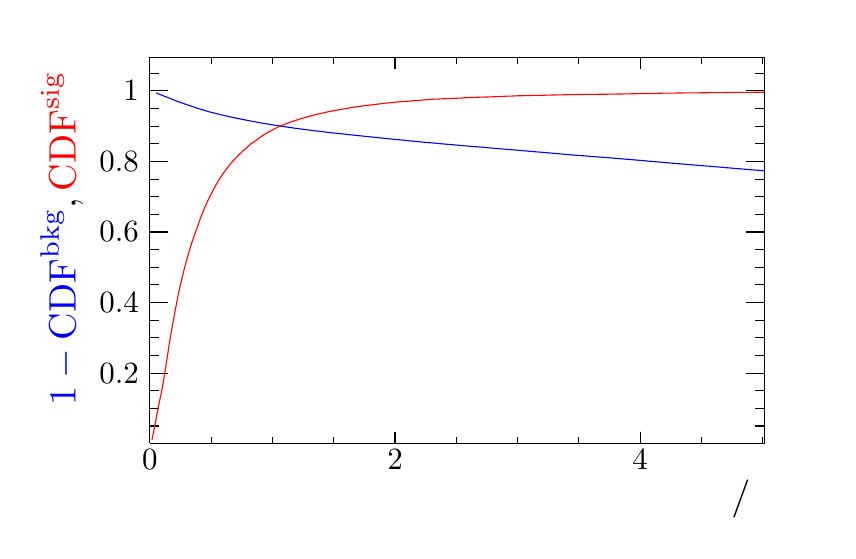
\begin{tikzpicture}
\pgfdeclareplotmark{cross} {
\pgfpathmoveto{\pgfpoint{-0.3\pgfplotmarksize}{\pgfplotmarksize}}
\pgfpathlineto{\pgfpoint{+0.3\pgfplotmarksize}{\pgfplotmarksize}}
\pgfpathlineto{\pgfpoint{+0.3\pgfplotmarksize}{0.3\pgfplotmarksize}}
\pgfpathlineto{\pgfpoint{+1\pgfplotmarksize}{0.3\pgfplotmarksize}}
\pgfpathlineto{\pgfpoint{+1\pgfplotmarksize}{-0.3\pgfplotmarksize}}
\pgfpathlineto{\pgfpoint{+0.3\pgfplotmarksize}{-0.3\pgfplotmarksize}}
\pgfpathlineto{\pgfpoint{+0.3\pgfplotmarksize}{-1.\pgfplotmarksize}}
\pgfpathlineto{\pgfpoint{-0.3\pgfplotmarksize}{-1.\pgfplotmarksize}}
\pgfpathlineto{\pgfpoint{-0.3\pgfplotmarksize}{-0.3\pgfplotmarksize}}
\pgfpathlineto{\pgfpoint{-1.\pgfplotmarksize}{-0.3\pgfplotmarksize}}
\pgfpathlineto{\pgfpoint{-1.\pgfplotmarksize}{0.3\pgfplotmarksize}}
\pgfpathlineto{\pgfpoint{-0.3\pgfplotmarksize}{0.3\pgfplotmarksize}}
\pgfpathclose
\pgfusepathqstroke
}
\pgfdeclareplotmark{cross*} {
\pgfpathmoveto{\pgfpoint{-0.3\pgfplotmarksize}{\pgfplotmarksize}}
\pgfpathlineto{\pgfpoint{+0.3\pgfplotmarksize}{\pgfplotmarksize}}
\pgfpathlineto{\pgfpoint{+0.3\pgfplotmarksize}{0.3\pgfplotmarksize}}
\pgfpathlineto{\pgfpoint{+1\pgfplotmarksize}{0.3\pgfplotmarksize}}
\pgfpathlineto{\pgfpoint{+1\pgfplotmarksize}{-0.3\pgfplotmarksize}}
\pgfpathlineto{\pgfpoint{+0.3\pgfplotmarksize}{-0.3\pgfplotmarksize}}
\pgfpathlineto{\pgfpoint{+0.3\pgfplotmarksize}{-1.\pgfplotmarksize}}
\pgfpathlineto{\pgfpoint{-0.3\pgfplotmarksize}{-1.\pgfplotmarksize}}
\pgfpathlineto{\pgfpoint{-0.3\pgfplotmarksize}{-0.3\pgfplotmarksize}}
\pgfpathlineto{\pgfpoint{-1.\pgfplotmarksize}{-0.3\pgfplotmarksize}}
\pgfpathlineto{\pgfpoint{-1.\pgfplotmarksize}{0.3\pgfplotmarksize}}
\pgfpathlineto{\pgfpoint{-0.3\pgfplotmarksize}{0.3\pgfplotmarksize}}
\pgfpathclose
\pgfusepathqfillstroke
}
\pgfdeclareplotmark{newstar} {
\pgfpathmoveto{\pgfqpoint{0pt}{\pgfplotmarksize}}
\pgfpathlineto{\pgfqpointpolar{44}{0.5\pgfplotmarksize}}
\pgfpathlineto{\pgfqpointpolar{18}{\pgfplotmarksize}}
\pgfpathlineto{\pgfqpointpolar{-20}{0.5\pgfplotmarksize}}
\pgfpathlineto{\pgfqpointpolar{-54}{\pgfplotmarksize}}
\pgfpathlineto{\pgfqpointpolar{-90}{0.5\pgfplotmarksize}}
\pgfpathlineto{\pgfqpointpolar{234}{\pgfplotmarksize}}
\pgfpathlineto{\pgfqpointpolar{198}{0.5\pgfplotmarksize}}
\pgfpathlineto{\pgfqpointpolar{162}{\pgfplotmarksize}}
\pgfpathlineto{\pgfqpointpolar{134}{0.5\pgfplotmarksize}}
\pgfpathclose
\pgfusepathqstroke
}
\pgfdeclareplotmark{newstar*} {
\pgfpathmoveto{\pgfqpoint{0pt}{\pgfplotmarksize}}
\pgfpathlineto{\pgfqpointpolar{44}{0.5\pgfplotmarksize}}
\pgfpathlineto{\pgfqpointpolar{18}{\pgfplotmarksize}}
\pgfpathlineto{\pgfqpointpolar{-20}{0.5\pgfplotmarksize}}
\pgfpathlineto{\pgfqpointpolar{-54}{\pgfplotmarksize}}
\pgfpathlineto{\pgfqpointpolar{-90}{0.5\pgfplotmarksize}}
\pgfpathlineto{\pgfqpointpolar{234}{\pgfplotmarksize}}
\pgfpathlineto{\pgfqpointpolar{198}{0.5\pgfplotmarksize}}
\pgfpathlineto{\pgfqpointpolar{162}{\pgfplotmarksize}}
\pgfpathlineto{\pgfqpointpolar{134}{0.5\pgfplotmarksize}}
\pgfpathclose
\pgfusepathqfillstroke
}
\definecolor{c}{rgb}{1,1,1};
\draw [color=c, fill=c] (0,0) rectangle (10,6.27517);
\draw [color=c, fill=c] (1.4,1.00403) rectangle (9.2,5.89866);
\definecolor{c}{rgb}{0,0,0};
\draw [c] (1.4,1.00403) -- (1.4,5.89866) -- (9.2,5.89866) -- (9.2,1.00403) -- (1.4,1.00403);
\definecolor{c}{rgb}{1,1,1};
\draw [color=c, fill=c] (1.4,1.00403) rectangle (9.2,5.89866);
\definecolor{c}{rgb}{0,0,0};
\draw [c] (1.4,1.00403) -- (1.4,5.89866) -- (9.2,5.89866) -- (9.2,1.00403) -- (1.4,1.00403);
\draw [c,line width=0.4] (1.4,1.00403) -- (9.2,1.00403);
\draw [anchor= east] (9.2,0.301208) node[scale=1.37879, rotate=0]{$\chisq/\nDoF$};
\draw [c,line width=0.4] (1.4,1.15087) -- (1.4,1.00403);
\draw [c,line width=0.4] (2.17838,1.07745) -- (2.17838,1.00403);
\draw [c,line width=0.4] (2.95677,1.07745) -- (2.95677,1.00403);
\draw [c,line width=0.4] (3.73515,1.07745) -- (3.73515,1.00403);
\draw [c,line width=0.4] (4.51354,1.15087) -- (4.51354,1.00403);
\draw [c,line width=0.4] (5.29192,1.07745) -- (5.29192,1.00403);
\draw [c,line width=0.4] (6.07031,1.07745) -- (6.07031,1.00403);
\draw [c,line width=0.4] (6.84869,1.07745) -- (6.84869,1.00403);
\draw [c,line width=0.4] (7.62707,1.15087) -- (7.62707,1.00403);
\draw [c,line width=0.4] (7.62707,1.15087) -- (7.62707,1.00403);
\draw [c,line width=0.4] (8.40546,1.07745) -- (8.40546,1.00403);
\draw [c,line width=0.4] (9.18384,1.07745) -- (9.18384,1.00403);
\draw [anchor=base] (1.4,0.665168) node[scale=1.11794, rotate=0]{0};
\draw [anchor=base] (4.51354,0.665168) node[scale=1.11794, rotate=0]{2};
\draw [anchor=base] (7.62707,0.665168) node[scale=1.11794, rotate=0]{4};
\draw [c,line width=0.4] (1.4,5.89866) -- (9.2,5.89866);
\draw [c,line width=0.4] (1.4,5.75182) -- (1.4,5.89866);
\draw [c,line width=0.4] (2.17838,5.82524) -- (2.17838,5.89866);
\draw [c,line width=0.4] (2.95677,5.82524) -- (2.95677,5.89866);
\draw [c,line width=0.4] (3.73515,5.82524) -- (3.73515,5.89866);
\draw [c,line width=0.4] (4.51354,5.75182) -- (4.51354,5.89866);
\draw [c,line width=0.4] (5.29192,5.82524) -- (5.29192,5.89866);
\draw [c,line width=0.4] (6.07031,5.82524) -- (6.07031,5.89866);
\draw [c,line width=0.4] (6.84869,5.82524) -- (6.84869,5.89866);
\draw [c,line width=0.4] (7.62707,5.75182) -- (7.62707,5.89866);
\draw [c,line width=0.4] (7.62707,5.75182) -- (7.62707,5.89866);
\draw [c,line width=0.4] (8.40546,5.82524) -- (8.40546,5.89866);
\draw [c,line width=0.4] (9.18384,5.82524) -- (9.18384,5.89866);
\draw [c,line width=0.4] (1.4,1.00403) -- (1.4,5.89866);
\draw [anchor= east] (0.28,5.89866) node[scale=1.37879, rotate=90]{${\color{blue} 1-{\rm CDF}^{\rm bkg}}, {\color{red} {\rm CDF}^{\rm sig}}$};
\draw [c,line width=0.4] (1.634,1.89519) -- (1.4,1.89519);
\draw [c,line width=0.4] (1.517,2.11921) -- (1.4,2.11921);
\draw [c,line width=0.4] (1.517,2.34323) -- (1.4,2.34323);
\draw [c,line width=0.4] (1.517,2.56724) -- (1.4,2.56724);
\draw [c,line width=0.4] (1.634,2.79126) -- (1.4,2.79126);
\draw [c,line width=0.4] (1.517,3.01528) -- (1.4,3.01528);
\draw [c,line width=0.4] (1.517,3.23929) -- (1.4,3.23929);
\draw [c,line width=0.4] (1.517,3.46331) -- (1.4,3.46331);
\draw [c,line width=0.4] (1.634,3.68733) -- (1.4,3.68733);
\draw [c,line width=0.4] (1.517,3.91134) -- (1.4,3.91134);
\draw [c,line width=0.4] (1.517,4.13536) -- (1.4,4.13536);
\draw [c,line width=0.4] (1.517,4.35938) -- (1.4,4.35938);
\draw [c,line width=0.4] (1.634,4.58339) -- (1.4,4.58339);
\draw [c,line width=0.4] (1.517,4.80741) -- (1.4,4.80741);
\draw [c,line width=0.4] (1.517,5.03143) -- (1.4,5.03143);
\draw [c,line width=0.4] (1.517,5.25544) -- (1.4,5.25544);
\draw [c,line width=0.4] (1.634,5.47946) -- (1.4,5.47946);
\draw [c,line width=0.4] (1.634,1.89519) -- (1.4,1.89519);
\draw [c,line width=0.4] (1.517,1.67118) -- (1.4,1.67118);
\draw [c,line width=0.4] (1.517,1.44716) -- (1.4,1.44716);
\draw [c,line width=0.4] (1.517,1.22314) -- (1.4,1.22314);
\draw [c,line width=0.4] (1.634,5.47946) -- (1.4,5.47946);
\draw [c,line width=0.4] (1.517,5.70348) -- (1.4,5.70348);
\draw [anchor= east] (1.4,1.89519) node[scale=1.11794, rotate=0]{0.2};
\draw [anchor= east] (1.4,2.79126) node[scale=1.11794, rotate=0]{0.4};
\draw [anchor= east] (1.4,3.68733) node[scale=1.11794, rotate=0]{0.6};
\draw [anchor= east] (1.4,4.58339) node[scale=1.11794, rotate=0]{0.8};
\draw [anchor= east] (1.4,5.47946) node[scale=1.11794, rotate=0]{1};
\draw [c,line width=0.4] (9.2,1.00403) -- (9.2,5.89866);
\draw [c,line width=0.4] (8.966,1.89519) -- (9.2,1.89519);
\draw [c,line width=0.4] (9.083,2.11921) -- (9.2,2.11921);
\draw [c,line width=0.4] (9.083,2.34323) -- (9.2,2.34323);
\draw [c,line width=0.4] (9.083,2.56724) -- (9.2,2.56724);
\draw [c,line width=0.4] (8.966,2.79126) -- (9.2,2.79126);
\draw [c,line width=0.4] (9.083,3.01528) -- (9.2,3.01528);
\draw [c,line width=0.4] (9.083,3.23929) -- (9.2,3.23929);
\draw [c,line width=0.4] (9.083,3.46331) -- (9.2,3.46331);
\draw [c,line width=0.4] (8.966,3.68733) -- (9.2,3.68733);
\draw [c,line width=0.4] (9.083,3.91134) -- (9.2,3.91134);
\draw [c,line width=0.4] (9.083,4.13536) -- (9.2,4.13536);
\draw [c,line width=0.4] (9.083,4.35938) -- (9.2,4.35938);
\draw [c,line width=0.4] (8.966,4.58339) -- (9.2,4.58339);
\draw [c,line width=0.4] (9.083,4.80741) -- (9.2,4.80741);
\draw [c,line width=0.4] (9.083,5.03143) -- (9.2,5.03143);
\draw [c,line width=0.4] (9.083,5.25544) -- (9.2,5.25544);
\draw [c,line width=0.4] (8.966,5.47946) -- (9.2,5.47946);
\draw [c,line width=0.4] (8.966,1.89519) -- (9.2,1.89519);
\draw [c,line width=0.4] (9.083,1.67118) -- (9.2,1.67118);
\draw [c,line width=0.4] (9.083,1.44716) -- (9.2,1.44716);
\draw [c,line width=0.4] (9.083,1.22314) -- (9.2,1.22314);
\draw [c,line width=0.4] (8.966,5.47946) -- (9.2,5.47946);
\draw [c,line width=0.4] (9.083,5.70348) -- (9.2,5.70348);
\definecolor{c}{rgb}{0,0,1};
\draw [c] (1.47874,5.45325) -- (1.61517,5.3993) -- (1.7516,5.34519) -- (1.88803,5.29811) -- (2.02445,5.252) -- (2.16088,5.21131) -- (2.29731,5.17735) -- (2.43374,5.14578) -- (2.57017,5.11844) -- (2.7066,5.09159) -- (2.84302,5.06689) --
 (2.97945,5.04451) -- (3.11588,5.02373) -- (3.25231,5.00407) -- (3.38874,4.98609) -- (3.52517,4.96962) -- (3.6616,4.95276) -- (3.79802,4.93781) -- (3.93445,4.92311) -- (4.07088,4.90872) -- (4.20731,4.89457) -- (4.34374,4.88067) -- (4.48017,4.86668)
 -- (4.6166,4.85381) -- (4.75302,4.83934) -- (4.88945,4.82656) -- (5.02588,4.81521) -- (5.16231,4.80242) -- (5.29874,4.79091) -- (5.43517,4.77796) -- (5.57159,4.76821) -- (5.70802,4.7563) -- (5.84445,4.74439) -- (5.98088,4.73328) -- (6.11731,4.72202)
 -- (6.25374,4.70955) -- (6.39017,4.69852) -- (6.52659,4.68661) -- (6.66302,4.67462) -- (6.79945,4.66271) -- (6.93588,4.6528) -- (7.07231,4.64169) -- (7.20874,4.63202) -- (7.34517,4.62043) -- (7.48159,4.60884) -- (7.61802,4.59773) --
 (7.75445,4.58566) -- (7.89088,4.57368) -- (8.02731,4.56145) -- (8.16374,4.55026) -- (8.30017,4.53883) -- (8.43659,4.52772) -- (8.57302,4.51709) -- (8.70945,4.50494) -- (8.84588,4.49359) -- (8.98231,4.48216) -- (9.11874,4.47089) -- (9.2,4.46456);
\definecolor{c}{rgb}{1,0,0};
\draw [c] (1.4261,1.04823) -- (1.45017,1.16505) -- (1.47424,1.28769) -- (1.49831,1.41856) -- (1.52238,1.53823) -- (1.54645,1.64968) -- (1.57052,1.77997) -- (1.59459,1.93162) -- (1.61866,2.08612) -- (1.64273,2.24428) -- (1.6668,2.38885) --
 (1.69087,2.52291) -- (1.71493,2.65674) -- (1.739,2.78292) -- (1.76307,2.90317) -- (1.78714,3.01245) -- (1.81121,3.11465) -- (1.83528,3.21103) -- (1.85935,3.30022) -- (1.88342,3.38986) -- (1.90749,3.47242) -- (1.93156,3.54836) -- (1.95563,3.61778) --
 (1.9797,3.68596) -- (2.00377,3.75196) -- (2.02784,3.82082) -- (2.05191,3.88853) -- (2.07597,3.94814) -- (2.10004,4.00764) -- (2.12411,4.05868) -- (2.14818,4.10881) -- (2.17225,4.15677) -- (2.19632,4.2045) -- (2.22039,4.25052) -- (2.24446,4.29392) --
 (2.26853,4.33571) -- (2.2926,4.37454) -- (2.31667,4.41051) -- (2.34074,4.44431) -- (2.36481,4.4756) -- (2.38888,4.507) -- (2.41295,4.53806) -- (2.43701,4.56992) -- (2.46108,4.59447) -- (2.48515,4.62074) -- (2.50922,4.64529) -- (2.53329,4.66961) --
 (2.55736,4.69222) -- (2.58143,4.71552) -- (2.6055,4.73847) -- (2.62957,4.75868) -- (2.65364,4.77981) -- (2.67771,4.80356) -- (2.70178,4.8192) -- (2.72585,4.83519) -- (2.74992,4.85106) -- (2.77399,4.86956) -- (2.79805,4.88772) -- (2.82212,4.90427) --
 (2.84619,4.92106) -- (2.87026,4.93511) -- (2.89433,4.94915) -- (2.9184,4.96217) -- (2.94247,4.97439) -- (2.96654,4.98889) -- (2.99061,5.00088) -- (3.01468,5.01299) -- (3.03875,5.02486) -- (3.06282,5.03651) -- (3.08689,5.04599) -- (3.11096,5.05512)
 -- (3.13503,5.06369) -- (3.1591,5.07294) -- (3.18316,5.08116) -- (3.20723,5.09018) -- (3.2313,5.09829) -- (3.25537,5.10617) -- (3.27944,5.11393) -- (3.30351,5.12181) -- (3.32758,5.12878) -- (3.35165,5.1362) -- (3.37572,5.14248) -- (3.39979,5.14945)
 -- (3.42386,5.15584) -- (3.44793,5.16155) -- (3.472,5.16932) -- (3.49607,5.17617) -- (3.52014,5.18302) -- (3.5442,5.18667) -- (3.56827,5.19147) -- (3.59234,5.19706) -- (3.61641,5.20266) -- (3.64048,5.20917) -- (3.66455,5.21442) -- (3.68862,5.2191)
 -- (3.71269,5.22333) -- (3.73676,5.22801) -- (3.76083,5.23223) -- (3.7849,5.23669) -- (3.80897,5.24091) -- (3.83304,5.24457) -- (3.85711,5.24936) -- (3.88118,5.25359) -- (3.90524,5.25713) -- (3.92931,5.2625) -- (3.95338,5.26661) -- (3.97745,5.27038)
 -- (4.00152,5.27437) -- (4.02559,5.2778) -- (4.04966,5.28054) -- (4.07373,5.28385) -- (4.0978,5.28728) -- (4.12187,5.29127) -- (4.14594,5.29378) -- (4.17001,5.2963) -- (4.19408,5.29927) -- (4.21815,5.30178) -- (4.24222,5.30498) -- (4.26628,5.30794)
 -- (4.29035,5.31091) -- (4.31442,5.31343) -- (4.33849,5.31662) -- (4.36256,5.31959) -- (4.38663,5.32279) -- (4.4107,5.32542) -- (4.43477,5.32701) -- (4.45884,5.32964) -- (4.48291,5.33192) -- (4.50698,5.33489) -- (4.53105,5.33752) --
 (4.55512,5.33946) -- (4.57919,5.34186) -- (4.60326,5.34403) -- (4.62732,5.34551) -- (4.65139,5.34654) -- (4.67546,5.34814) -- (4.69953,5.35031) -- (4.7236,5.35214) -- (4.74767,5.35408) -- (4.77174,5.35568) -- (4.79581,5.35739) -- (4.81988,5.35922)
 -- (4.84395,5.36116) -- (4.86802,5.36299) -- (4.89209,5.3647) -- (4.91616,5.36675) -- (4.94023,5.36961) -- (4.9643,5.37109) -- (4.98836,5.37292) -- (5.01243,5.37395) -- (5.0365,5.37486) -- (5.06057,5.37555) -- (5.08464,5.37703) -- (5.10871,5.37794)
 -- (5.13278,5.3792) -- (5.15685,5.38057) -- (5.18092,5.38137) -- (5.20499,5.3824) -- (5.22906,5.38274) -- (5.25313,5.38434) -- (5.2772,5.3856) -- (5.30127,5.38617) -- (5.32534,5.38731) -- (5.34941,5.38799) -- (5.37347,5.38971) -- (5.39754,5.39165)
 -- (5.42161,5.39302) -- (5.44568,5.39416) -- (5.46975,5.39496) -- (5.49382,5.39576) -- (5.51789,5.39656) -- (5.54196,5.3977) -- (5.56603,5.3985) -- (5.5901,5.39953) -- (5.61417,5.4001) -- (5.63824,5.40067) -- (5.66231,5.40135) -- (5.68638,5.40193)
 -- (5.71045,5.40272) -- (5.73451,5.40318) -- (5.75858,5.40444) -- (5.78265,5.40546) -- (5.80672,5.40604) -- (5.83079,5.40695) -- (5.85486,5.40798) -- (5.87893,5.40946) -- (5.903,5.41003) -- (5.92707,5.41186) -- (5.95114,5.41254) -- (5.97521,5.413)
 -- (5.99928,5.4138) -- (6.02335,5.41471) -- (6.04742,5.41643) -- (6.07149,5.417) -- (6.09555,5.41723) -- (6.11962,5.4178) -- (6.14369,5.41848) -- (6.16776,5.41928) -- (6.19183,5.42042) -- (6.2159,5.42099) -- (6.23997,5.42122) -- (6.26404,5.42157) --
 (6.28811,5.42191) -- (6.31218,5.42237) -- (6.33625,5.42271) -- (6.36032,5.42305) -- (6.38439,5.42351) -- (6.40846,5.42408) -- (6.43253,5.42499) -- (6.45659,5.42591) -- (6.48066,5.42625) -- (6.50473,5.42648) -- (6.5288,5.42705) -- (6.55287,5.42773)
 -- (6.57694,5.42796) -- (6.60101,5.42807) -- (6.62508,5.42865) -- (6.64915,5.42945) -- (6.67322,5.43013) -- (6.69729,5.43082) -- (6.72136,5.4315) -- (6.74543,5.43161) -- (6.7695,5.43207) -- (6.79357,5.43241) -- (6.81764,5.43276) -- (6.8417,5.43298)
 -- (6.86577,5.4331) -- (6.88984,5.43356) -- (6.91391,5.43424) -- (6.93798,5.43447) -- (6.96205,5.43458) -- (6.98612,5.43481) -- (7.01019,5.43515) -- (7.03426,5.43538) -- (7.05833,5.43573) -- (7.0824,5.43584) -- (7.10647,5.43607) -- (7.13054,5.43618)
 -- (7.15461,5.4363) -- (7.17868,5.43664) -- (7.20274,5.43721) -- (7.22681,5.43755) -- (7.25088,5.43801) -- (7.27495,5.43835) -- (7.29902,5.43881) -- (7.32309,5.43927) -- (7.34716,5.43972) -- (7.37123,5.44006) -- (7.3953,5.44029) -- (7.41937,5.44064)
 -- (7.44344,5.44098) -- (7.46751,5.44121) -- (7.49158,5.44178) -- (7.51565,5.44258) -- (7.53972,5.44258) -- (7.56378,5.4436) -- (7.58785,5.44372) -- (7.61192,5.44452) -- (7.63599,5.44486) -- (7.66006,5.44532) -- (7.68413,5.44577) -- (7.7082,5.44646)
 -- (7.73227,5.44657) -- (7.75634,5.44669) -- (7.78041,5.44703) -- (7.80448,5.4476) -- (7.82855,5.44794) -- (7.85262,5.44874) -- (7.87669,5.44931) -- (7.90076,5.44977) -- (7.92483,5.45034) -- (7.94889,5.45034) -- (7.97296,5.45034) --
 (7.99703,5.45046) -- (8.0211,5.45114) -- (8.04517,5.45148) -- (8.06924,5.45171) -- (8.09331,5.45194) -- (8.11738,5.45274) -- (8.14145,5.45274) -- (8.16552,5.4532) -- (8.18959,5.45331) -- (8.21366,5.45343) -- (8.23773,5.45354) -- (8.2618,5.45377) --
 (8.28587,5.454) -- (8.30993,5.45411) -- (8.334,5.45434) -- (8.35807,5.45457) -- (8.38214,5.45502) -- (8.40621,5.45537) -- (8.43028,5.45548) -- (8.45435,5.45571) -- (8.47842,5.45605) -- (8.50249,5.45639) -- (8.52656,5.45651) -- (8.55063,5.45685) --
 (8.5747,5.45697) -- (8.59877,5.45708) -- (8.62284,5.45742) -- (8.6469,5.45765) -- (8.67097,5.45799) -- (8.69504,5.45811) -- (8.71911,5.45868) -- (8.74318,5.45891) -- (8.76725,5.45925) -- (8.79132,5.45936) -- (8.81539,5.45948) -- (8.83946,5.45971) --
 (8.86353,5.45993) -- (8.8876,5.46016) -- (8.91167,5.46028) -- (8.93574,5.46051) -- (8.95981,5.46051) -- (8.98388,5.46073) -- (9.00795,5.46085) -- (9.03201,5.46096) -- (9.05608,5.46119) -- (9.08015,5.46153) -- (9.10422,5.46153) -- (9.12829,5.46153)
 -- (9.15236,5.46165) -- (9.17643,5.46199) -- (9.2,5.46233) -- (9.2,5.46233);
\end{tikzpicture}
}
    \caption{}
    \label{mvm_cdf}
  \end{subfigure}%
  \hfill%
  \begin{subfigure}{0.5\textwidth}
    \raggedleft
    \tikzsetnextfilename{roc_curve_mvm}
    \scalebox{0.55}{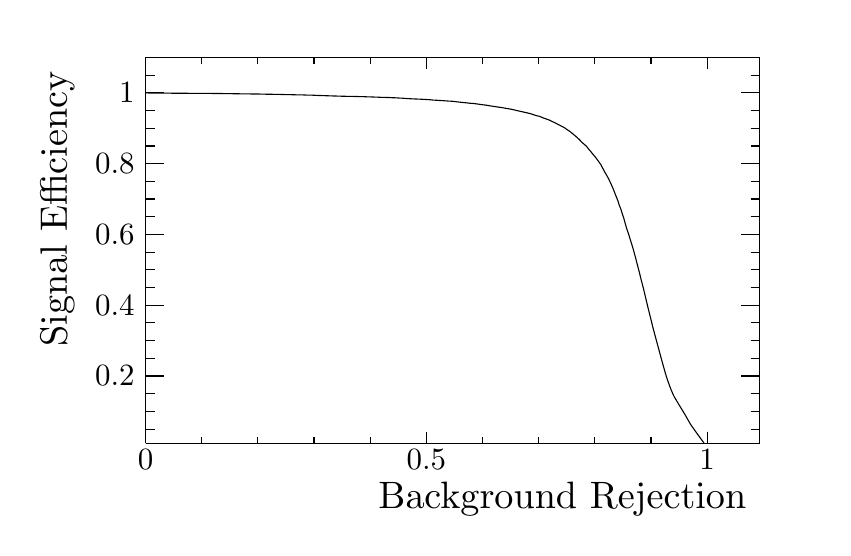
\begin{tikzpicture}
\pgfdeclareplotmark{cross} {
\pgfpathmoveto{\pgfpoint{-0.3\pgfplotmarksize}{\pgfplotmarksize}}
\pgfpathlineto{\pgfpoint{+0.3\pgfplotmarksize}{\pgfplotmarksize}}
\pgfpathlineto{\pgfpoint{+0.3\pgfplotmarksize}{0.3\pgfplotmarksize}}
\pgfpathlineto{\pgfpoint{+1\pgfplotmarksize}{0.3\pgfplotmarksize}}
\pgfpathlineto{\pgfpoint{+1\pgfplotmarksize}{-0.3\pgfplotmarksize}}
\pgfpathlineto{\pgfpoint{+0.3\pgfplotmarksize}{-0.3\pgfplotmarksize}}
\pgfpathlineto{\pgfpoint{+0.3\pgfplotmarksize}{-1.\pgfplotmarksize}}
\pgfpathlineto{\pgfpoint{-0.3\pgfplotmarksize}{-1.\pgfplotmarksize}}
\pgfpathlineto{\pgfpoint{-0.3\pgfplotmarksize}{-0.3\pgfplotmarksize}}
\pgfpathlineto{\pgfpoint{-1.\pgfplotmarksize}{-0.3\pgfplotmarksize}}
\pgfpathlineto{\pgfpoint{-1.\pgfplotmarksize}{0.3\pgfplotmarksize}}
\pgfpathlineto{\pgfpoint{-0.3\pgfplotmarksize}{0.3\pgfplotmarksize}}
\pgfpathclose
\pgfusepathqstroke
}
\pgfdeclareplotmark{cross*} {
\pgfpathmoveto{\pgfpoint{-0.3\pgfplotmarksize}{\pgfplotmarksize}}
\pgfpathlineto{\pgfpoint{+0.3\pgfplotmarksize}{\pgfplotmarksize}}
\pgfpathlineto{\pgfpoint{+0.3\pgfplotmarksize}{0.3\pgfplotmarksize}}
\pgfpathlineto{\pgfpoint{+1\pgfplotmarksize}{0.3\pgfplotmarksize}}
\pgfpathlineto{\pgfpoint{+1\pgfplotmarksize}{-0.3\pgfplotmarksize}}
\pgfpathlineto{\pgfpoint{+0.3\pgfplotmarksize}{-0.3\pgfplotmarksize}}
\pgfpathlineto{\pgfpoint{+0.3\pgfplotmarksize}{-1.\pgfplotmarksize}}
\pgfpathlineto{\pgfpoint{-0.3\pgfplotmarksize}{-1.\pgfplotmarksize}}
\pgfpathlineto{\pgfpoint{-0.3\pgfplotmarksize}{-0.3\pgfplotmarksize}}
\pgfpathlineto{\pgfpoint{-1.\pgfplotmarksize}{-0.3\pgfplotmarksize}}
\pgfpathlineto{\pgfpoint{-1.\pgfplotmarksize}{0.3\pgfplotmarksize}}
\pgfpathlineto{\pgfpoint{-0.3\pgfplotmarksize}{0.3\pgfplotmarksize}}
\pgfpathclose
\pgfusepathqfillstroke
}
\pgfdeclareplotmark{newstar} {
\pgfpathmoveto{\pgfqpoint{0pt}{\pgfplotmarksize}}
\pgfpathlineto{\pgfqpointpolar{44}{0.5\pgfplotmarksize}}
\pgfpathlineto{\pgfqpointpolar{18}{\pgfplotmarksize}}
\pgfpathlineto{\pgfqpointpolar{-20}{0.5\pgfplotmarksize}}
\pgfpathlineto{\pgfqpointpolar{-54}{\pgfplotmarksize}}
\pgfpathlineto{\pgfqpointpolar{-90}{0.5\pgfplotmarksize}}
\pgfpathlineto{\pgfqpointpolar{234}{\pgfplotmarksize}}
\pgfpathlineto{\pgfqpointpolar{198}{0.5\pgfplotmarksize}}
\pgfpathlineto{\pgfqpointpolar{162}{\pgfplotmarksize}}
\pgfpathlineto{\pgfqpointpolar{134}{0.5\pgfplotmarksize}}
\pgfpathclose
\pgfusepathqstroke
}
\pgfdeclareplotmark{newstar*} {
\pgfpathmoveto{\pgfqpoint{0pt}{\pgfplotmarksize}}
\pgfpathlineto{\pgfqpointpolar{44}{0.5\pgfplotmarksize}}
\pgfpathlineto{\pgfqpointpolar{18}{\pgfplotmarksize}}
\pgfpathlineto{\pgfqpointpolar{-20}{0.5\pgfplotmarksize}}
\pgfpathlineto{\pgfqpointpolar{-54}{\pgfplotmarksize}}
\pgfpathlineto{\pgfqpointpolar{-90}{0.5\pgfplotmarksize}}
\pgfpathlineto{\pgfqpointpolar{234}{\pgfplotmarksize}}
\pgfpathlineto{\pgfqpointpolar{198}{0.5\pgfplotmarksize}}
\pgfpathlineto{\pgfqpointpolar{162}{\pgfplotmarksize}}
\pgfpathlineto{\pgfqpointpolar{134}{0.5\pgfplotmarksize}}
\pgfpathclose
\pgfusepathqfillstroke
}
\definecolor{c}{rgb}{1,1,1};
\draw [color=c, fill=c] (0,0) rectangle (10,6.27517);
\draw [color=c, fill=c] (1.4,1.00403) rectangle (9.2,5.89866);
\definecolor{c}{rgb}{0,0,0};
\draw [c] (1.4,1.00403) -- (1.4,5.89866) -- (9.2,5.89866) -- (9.2,1.00403) -- (1.4,1.00403);
\draw [c,line width=0.4] (1.4,1.00403) -- (9.2,1.00403);
\draw [anchor= east] (9.2,0.301208) node[scale=1.37879, rotate=0]{Background Rejection};
\draw [c,line width=0.4] (1.4,1.15087) -- (1.4,1.00403);
\draw [c,line width=0.4] (2.11326,1.07745) -- (2.11326,1.00403);
\draw [c,line width=0.4] (2.82653,1.07745) -- (2.82653,1.00403);
\draw [c,line width=0.4] (3.53979,1.07745) -- (3.53979,1.00403);
\draw [c,line width=0.4] (4.25306,1.07745) -- (4.25306,1.00403);
\draw [c,line width=0.4] (4.96632,1.15087) -- (4.96632,1.00403);
\draw [c,line width=0.4] (5.67959,1.07745) -- (5.67959,1.00403);
\draw [c,line width=0.4] (6.39285,1.07745) -- (6.39285,1.00403);
\draw [c,line width=0.4] (7.10611,1.07745) -- (7.10611,1.00403);
\draw [c,line width=0.4] (7.81938,1.07745) -- (7.81938,1.00403);
\draw [c,line width=0.4] (8.53264,1.15087) -- (8.53264,1.00403);
\draw [c,line width=0.4] (8.53264,1.15087) -- (8.53264,1.00403);
\draw [anchor=base] (1.4,0.665168) node[scale=1.11794, rotate=0]{0};
\draw [anchor=base] (4.96632,0.665168) node[scale=1.11794, rotate=0]{0.5};
\draw [anchor=base] (8.53264,0.665168) node[scale=1.11794, rotate=0]{1};
\draw [c,line width=0.4] (1.4,5.89866) -- (9.2,5.89866);
\draw [c,line width=0.4] (1.4,5.75182) -- (1.4,5.89866);
\draw [c,line width=0.4] (2.11326,5.82524) -- (2.11326,5.89866);
\draw [c,line width=0.4] (2.82653,5.82524) -- (2.82653,5.89866);
\draw [c,line width=0.4] (3.53979,5.82524) -- (3.53979,5.89866);
\draw [c,line width=0.4] (4.25306,5.82524) -- (4.25306,5.89866);
\draw [c,line width=0.4] (4.96632,5.75182) -- (4.96632,5.89866);
\draw [c,line width=0.4] (5.67959,5.82524) -- (5.67959,5.89866);
\draw [c,line width=0.4] (6.39285,5.82524) -- (6.39285,5.89866);
\draw [c,line width=0.4] (7.10611,5.82524) -- (7.10611,5.89866);
\draw [c,line width=0.4] (7.81938,5.82524) -- (7.81938,5.89866);
\draw [c,line width=0.4] (8.53264,5.75182) -- (8.53264,5.89866);
\draw [c,line width=0.4] (8.53264,5.75182) -- (8.53264,5.89866);
\draw [c,line width=0.4] (1.4,1.00403) -- (1.4,5.89866);
\draw [anchor= east] (0.28,5.89866) node[scale=1.37879, rotate=90]{Signal Efficiency};
\draw [c,line width=0.4] (1.634,1.85858) -- (1.4,1.85858);
\draw [c,line width=0.4] (1.517,2.08331) -- (1.4,2.08331);
\draw [c,line width=0.4] (1.517,2.30803) -- (1.4,2.30803);
\draw [c,line width=0.4] (1.517,2.53275) -- (1.4,2.53275);
\draw [c,line width=0.4] (1.634,2.75747) -- (1.4,2.75747);
\draw [c,line width=0.4] (1.517,2.9822) -- (1.4,2.9822);
\draw [c,line width=0.4] (1.517,3.20692) -- (1.4,3.20692);
\draw [c,line width=0.4] (1.517,3.43164) -- (1.4,3.43164);
\draw [c,line width=0.4] (1.634,3.65636) -- (1.4,3.65636);
\draw [c,line width=0.4] (1.517,3.88108) -- (1.4,3.88108);
\draw [c,line width=0.4] (1.517,4.10581) -- (1.4,4.10581);
\draw [c,line width=0.4] (1.517,4.33053) -- (1.4,4.33053);
\draw [c,line width=0.4] (1.634,4.55525) -- (1.4,4.55525);
\draw [c,line width=0.4] (1.517,4.77997) -- (1.4,4.77997);
\draw [c,line width=0.4] (1.517,5.00469) -- (1.4,5.00469);
\draw [c,line width=0.4] (1.517,5.22942) -- (1.4,5.22942);
\draw [c,line width=0.4] (1.634,5.45414) -- (1.4,5.45414);
\draw [c,line width=0.4] (1.634,1.85858) -- (1.4,1.85858);
\draw [c,line width=0.4] (1.517,1.63386) -- (1.4,1.63386);
\draw [c,line width=0.4] (1.517,1.40914) -- (1.4,1.40914);
\draw [c,line width=0.4] (1.517,1.18442) -- (1.4,1.18442);
\draw [c,line width=0.4] (1.634,5.45414) -- (1.4,5.45414);
\draw [c,line width=0.4] (1.517,5.67886) -- (1.4,5.67886);
\draw [anchor= east] (1.4,1.85858) node[scale=1.11794, rotate=0]{0.2};
\draw [anchor= east] (1.4,2.75747) node[scale=1.11794, rotate=0]{0.4};
\draw [anchor= east] (1.4,3.65636) node[scale=1.11794, rotate=0]{0.6};
\draw [anchor= east] (1.4,4.55525) node[scale=1.11794, rotate=0]{0.8};
\draw [anchor= east] (1.4,5.45414) node[scale=1.11794, rotate=0]{1};
\draw [c,line width=0.4] (9.2,1.00403) -- (9.2,5.89866);
\draw [c,line width=0.4] (8.966,1.85858) -- (9.2,1.85858);
\draw [c,line width=0.4] (9.083,2.08331) -- (9.2,2.08331);
\draw [c,line width=0.4] (9.083,2.30803) -- (9.2,2.30803);
\draw [c,line width=0.4] (9.083,2.53275) -- (9.2,2.53275);
\draw [c,line width=0.4] (8.966,2.75747) -- (9.2,2.75747);
\draw [c,line width=0.4] (9.083,2.9822) -- (9.2,2.9822);
\draw [c,line width=0.4] (9.083,3.20692) -- (9.2,3.20692);
\draw [c,line width=0.4] (9.083,3.43164) -- (9.2,3.43164);
\draw [c,line width=0.4] (8.966,3.65636) -- (9.2,3.65636);
\draw [c,line width=0.4] (9.083,3.88108) -- (9.2,3.88108);
\draw [c,line width=0.4] (9.083,4.10581) -- (9.2,4.10581);
\draw [c,line width=0.4] (9.083,4.33053) -- (9.2,4.33053);
\draw [c,line width=0.4] (8.966,4.55525) -- (9.2,4.55525);
\draw [c,line width=0.4] (9.083,4.77997) -- (9.2,4.77997);
\draw [c,line width=0.4] (9.083,5.00469) -- (9.2,5.00469);
\draw [c,line width=0.4] (9.083,5.22942) -- (9.2,5.22942);
\draw [c,line width=0.4] (8.966,5.45414) -- (9.2,5.45414);
\draw [c,line width=0.4] (8.966,1.85858) -- (9.2,1.85858);
\draw [c,line width=0.4] (9.083,1.63386) -- (9.2,1.63386);
\draw [c,line width=0.4] (9.083,1.40914) -- (9.2,1.40914);
\draw [c,line width=0.4] (9.083,1.18442) -- (9.2,1.18442);
\draw [c,line width=0.4] (8.966,5.45414) -- (9.2,5.45414);
\draw [c,line width=0.4] (9.083,5.67886) -- (9.2,5.67886);
\draw [c] (8.49091,1.00895) -- (8.40502,1.12614) -- (8.32591,1.23809) -- (8.31888,1.24917) -- (8.24394,1.38044) -- (8.17052,1.50049) -- (8.11658,1.59074) -- (8.10576,1.6123) -- (8.07195,1.69003) -- (8.05168,1.743) -- (8.01718,1.84432) --
 (8.00142,1.89513) -- (7.9579,2.05011) -- (7.91515,2.20877) -- (7.87584,2.35379) -- (7.84021,2.48828) -- (7.80713,2.62253) -- (7.77583,2.74911) -- (7.7472,2.86973) -- (7.72099,2.97936) -- (7.69414,3.08188) -- (7.67034,3.17857) -- (7.64693,3.26803) --
 (7.62403,3.35795) -- (7.60151,3.44078) -- (7.57937,3.51695) -- (7.5571,3.5866) -- (7.53662,3.65499) -- (7.51359,3.7212) -- (7.49323,3.79027) -- (7.47516,3.8582) -- (7.4548,3.918) -- (7.43648,3.97768) -- (7.41587,4.02888) -- (7.40034,4.07917) --
 (7.38138,4.12728) -- (7.36243,4.17517) -- (7.34474,4.22133) -- (7.3268,4.26486) -- (7.30695,4.30679) -- (7.28939,4.34574) -- (7.27043,4.38182) -- (7.25135,4.41573) -- (7.23239,4.44711) -- (7.21661,4.47862) -- (7.19892,4.50977) -- (7.18353,4.54173)
 -- (7.16508,4.56636) -- (7.14663,4.59271) -- (7.12894,4.61734) -- (7.10973,4.64174) -- (7.09064,4.66442) -- (7.07118,4.68779) -- (7.05336,4.71081) -- (7.03517,4.73109) -- (7.01748,4.75228) -- (7.00056,4.77611) -- (6.98122,4.7918) --
 (6.96315,4.80784) -- (6.94495,4.82376) -- (6.92701,4.84232) -- (6.91009,4.86053) -- (6.89177,4.87714) -- (6.87319,4.89398) -- (6.8583,4.90807) -- (6.83947,4.92216) -- (6.82471,4.93522) -- (6.80906,4.94748) -- (6.79125,4.96202) -- (6.7742,4.97405) --
 (6.75549,4.98619) -- (6.73819,4.99811) -- (6.72318,5.00979) -- (6.706,5.0193) -- (6.68882,5.02846) -- (6.67101,5.03706) -- (6.65421,5.04633) -- (6.63525,5.05458) -- (6.62088,5.06363) -- (6.60497,5.07176) -- (6.58843,5.07967) -- (6.57036,5.08746) --
 (6.55433,5.09536) -- (6.53855,5.10235) -- (6.5243,5.1098) -- (6.50611,5.1161) -- (6.48804,5.12308) -- (6.46984,5.1295) -- (6.45178,5.13523) -- (6.43523,5.14302) -- (6.41844,5.14989) -- (6.40126,5.15676) -- (6.38294,5.16043) -- (6.36411,5.16524) --
 (6.34578,5.17085) -- (6.32861,5.17647) -- (6.31067,5.18299) -- (6.29349,5.18826) -- (6.27644,5.19296) -- (6.25875,5.1972) -- (6.24005,5.2019) -- (6.21816,5.20613) -- (6.19921,5.2106) -- (6.18254,5.21484) -- (6.16269,5.21851) -- (6.14487,5.22332) --
 (6.12553,5.22756) -- (6.10785,5.23111) -- (6.08749,5.23649) -- (6.07006,5.24061) -- (6.05275,5.24439) -- (6.03239,5.2484) -- (6.01344,5.25184) -- (5.9946,5.25459) -- (5.97603,5.25791) -- (5.95707,5.26135) -- (5.93798,5.26536) -- (5.92119,5.26788) --
 (5.90108,5.2704) -- (5.88187,5.27338) -- (5.86177,5.2759) -- (5.84294,5.2791) -- (5.82372,5.28208) -- (5.80336,5.28506) -- (5.78631,5.28758) -- (5.76774,5.29079) -- (5.75107,5.29377) -- (5.73198,5.29697) -- (5.71315,5.29961) -- (5.6961,5.30121) --
 (5.67816,5.30385) -- (5.65755,5.30614) -- (5.64101,5.30912) -- (5.62396,5.31175) -- (5.60703,5.3137) -- (5.59037,5.3161) -- (5.5737,5.31828) -- (5.55538,5.31977) -- (5.53705,5.3208) -- (5.51873,5.3224) -- (5.50028,5.32458) -- (5.48527,5.32641) --
 (5.46898,5.32836) -- (5.45078,5.32996) -- (5.43246,5.33168) -- (5.41579,5.33352) -- (5.39811,5.33546) -- (5.3822,5.3373) -- (5.36681,5.33901) -- (5.34683,5.34108) -- (5.32965,5.34394) -- (5.31324,5.34543) -- (5.29683,5.34726) -- (5.27876,5.34829) --
 (5.26158,5.34921) -- (5.24529,5.3499) -- (5.22888,5.35139) -- (5.21552,5.3523) -- (5.19961,5.35356) -- (5.18295,5.35494) -- (5.16577,5.35574) -- (5.15037,5.35677) -- (5.13485,5.35711) -- (5.11729,5.35872) -- (5.10329,5.35998) -- (5.08446,5.36055) --
 (5.06792,5.3617) -- (5.05342,5.36238) -- (5.03866,5.3641) -- (5.02326,5.36605) -- (5.00647,5.36742) -- (4.98852,5.36857) -- (4.97313,5.36937) -- (4.9571,5.37017) -- (4.93839,5.37097) -- (4.92312,5.37212) -- (4.90773,5.37292) -- (4.89081,5.37395) --
 (4.87528,5.37453) -- (4.86014,5.3751) -- (4.84487,5.37579) -- (4.82897,5.37636) -- (4.81077,5.37716) -- (4.79512,5.37762) -- (4.77616,5.37888) -- (4.7614,5.37991) -- (4.74346,5.38048) -- (4.72845,5.3814) -- (4.71292,5.38243) -- (4.69664,5.38392) --
 (4.68175,5.38449) -- (4.66483,5.38632) -- (4.65096,5.38701) -- (4.63556,5.38747) -- (4.62208,5.38827) -- (4.60592,5.38919) -- (4.5909,5.39091) -- (4.57385,5.39148) -- (4.55731,5.39171) -- (4.54204,5.39228) -- (4.5269,5.39297) -- (4.51138,5.39377) --
 (4.49675,5.39492) -- (4.48288,5.39549) -- (4.46545,5.39572) -- (4.45094,5.39606) -- (4.43554,5.3964) -- (4.42015,5.39686) -- (4.40361,5.39721) -- (4.39025,5.39755) -- (4.37714,5.39801) -- (4.3634,5.39858) -- (4.34877,5.3995) -- (4.33375,5.40041) --
 (4.31798,5.40076) -- (4.30322,5.40099) -- (4.28909,5.40156) -- (4.27637,5.40225) -- (4.25995,5.40248) -- (4.24278,5.40259) -- (4.22713,5.40316) -- (4.21237,5.40397) -- (4.19748,5.40465) -- (4.18081,5.40534) -- (4.16402,5.40603) -- (4.149,5.40614) --
 (4.135,5.4066) -- (4.12012,5.40694) -- (4.10587,5.40729) -- (4.08971,5.40752) -- (4.0752,5.40763) -- (4.0607,5.40809) -- (4.04797,5.40878) -- (4.0336,5.40901) -- (4.02011,5.40912) -- (4.00522,5.40935) -- (3.99275,5.40969) -- (3.97926,5.40992) --
 (3.96692,5.41027) -- (3.95229,5.41038) -- (3.93791,5.41061) -- (3.92506,5.41072) -- (3.91335,5.41084) -- (3.89974,5.41118) -- (3.88778,5.41176) -- (3.87658,5.4121) -- (3.86259,5.41256) -- (3.84884,5.4129) -- (3.83714,5.41336) -- (3.82403,5.41382) --
 (3.81258,5.41428) -- (3.79897,5.41462) -- (3.78599,5.41485) -- (3.77161,5.41519) -- (3.76054,5.41554) -- (3.74896,5.41576) -- (3.73687,5.41634) -- (3.72186,5.41714) -- (3.70837,5.41714) -- (3.69616,5.41817) -- (3.68203,5.41828) -- (3.66804,5.41909)
 -- (3.65519,5.41943) -- (3.64272,5.41989) -- (3.62948,5.42035) -- (3.61676,5.42103) -- (3.60722,5.42115) -- (3.59475,5.42126) -- (3.58164,5.42161) -- (3.57045,5.42218) -- (3.55988,5.42252) -- (3.55021,5.42332) -- (3.53991,5.4239) --
 (3.52744,5.42436) -- (3.517,5.42493) -- (3.50454,5.42493) -- (3.49321,5.42493) -- (3.48303,5.42504) -- (3.4698,5.42573) -- (3.45669,5.42607) -- (3.44613,5.4263) -- (3.43532,5.42653) -- (3.42463,5.42733) -- (3.4128,5.42733) -- (3.40376,5.42779) --
 (3.39435,5.42791) -- (3.38264,5.42802) -- (3.37043,5.42814) -- (3.35948,5.42837) -- (3.3465,5.42859) -- (3.3348,5.42871) -- (3.32449,5.42894) -- (3.31329,5.42917) -- (3.30286,5.42963) -- (3.29243,5.42997) -- (3.28123,5.43008) -- (3.27118,5.43031) --
 (3.26176,5.43066) -- (3.25273,5.431) -- (3.24408,5.43111) -- (3.23275,5.43146) -- (3.22092,5.43157) -- (3.20743,5.43169) -- (3.19942,5.43203) -- (3.18771,5.43226) -- (3.17842,5.4326) -- (3.16837,5.43272) -- (3.15577,5.43329) -- (3.14661,5.43352) --
 (3.13707,5.43386) -- (3.12689,5.43398) -- (3.11557,5.43409) -- (3.10768,5.43432) -- (3.09877,5.43455) -- (3.08783,5.43478) -- (3.07727,5.43489) -- (3.06658,5.43512) -- (3.05551,5.43512) -- (3.0466,5.43535) -- (3.03744,5.43547) -- (3.02777,5.43558)
 -- (3.01645,5.43581) -- (3.00779,5.43615) -- (2.99774,5.43615) -- (2.98629,5.43615) -- (2.97726,5.43627) -- (2.96848,5.43661) -- (2.95855,5.43696) -- (2.94761,5.43707) -- (2.9373,5.43707) -- (2.92763,5.43719) -- (2.91796,5.43753) --
 (2.90982,5.43776) -- (2.90028,5.43799) -- (2.8901,5.43822) -- (2.88005,5.43845) -- (2.86732,5.43867) -- (2.85702,5.4389) -- (2.84798,5.43913) -- (2.83882,5.43913) -- (2.83042,5.43936) -- (2.82012,5.43971) -- (2.80981,5.43971) -- (2.80039,5.43971) --
 (2.78996,5.43982) -- (2.78042,5.43993) -- (2.77316,5.44005) -- (2.76477,5.44005) -- (2.75764,5.44016) -- (2.74835,5.44039) -- (2.73957,5.44039) -- (2.73118,5.44062) -- (2.7224,5.44062) -- (2.7126,5.44085) -- (2.70535,5.44085) -- (2.69631,5.44085) --
 (2.6883,5.44085) -- (2.68066,5.44085) -- (2.67188,5.44097) -- (2.66399,5.44108) -- (2.65521,5.4412) -- (2.6472,5.44131) -- (2.63893,5.44131) -- (2.63167,5.44154) -- (2.62442,5.44165) -- (2.61539,5.44188) -- (2.60839,5.442) -- (2.60101,5.442) --
 (2.59478,5.44234) -- (2.58625,5.44234) -- (2.57645,5.44234) -- (2.56844,5.44257) -- (2.56106,5.44257) -- (2.55228,5.4428) -- (2.5449,5.4428) -- (2.53714,5.44291) -- (2.52899,5.44314) -- (2.52314,5.44337) -- (2.51589,5.44349) -- (2.50825,5.4436) --
 (2.50011,5.44372) -- (2.4926,5.44394) -- (2.48497,5.44406) -- (2.47784,5.44406) -- (2.4697,5.44406) -- (2.46245,5.44417) -- (2.45825,5.44417) -- (2.45061,5.44429) -- (2.44451,5.44429) -- (2.43687,5.44452) -- (2.43102,5.44475) -- (2.42504,5.44475) --
 (2.41817,5.44486) -- (2.41041,5.44497) -- (2.40239,5.44509) -- (2.39488,5.4452) -- (2.38687,5.4452) -- (2.38178,5.44543) -- (2.37503,5.44555) -- (2.3688,5.44555) -- (2.36206,5.44566) -- (2.35468,5.44578) -- (2.34844,5.44578) -- (2.34144,5.44589) --
 (2.33304,5.44589) -- (2.3235,5.44589) -- (2.31752,5.44589) -- (2.31103,5.44589) -- (2.30543,5.44589) -- (2.29996,5.44589) -- (2.29347,5.44589) -- (2.28737,5.44601) -- (2.28011,5.44624) -- (2.27413,5.44635) -- (2.26853,5.44635) -- (2.26268,5.44635)
 -- (2.25645,5.44658) -- (2.25059,5.44669) -- (2.24207,5.44681) -- (2.23558,5.44692) -- (2.22884,5.44692) -- (2.22387,5.44692) -- (2.21967,5.44692) -- (2.21382,5.44692) -- (2.20657,5.44704) -- (2.20072,5.44727) -- (2.19435,5.4475) --
 (2.18659,5.44761) -- (2.17947,5.44761) -- (2.17476,5.44761) -- (2.16891,5.44761) -- (2.16407,5.44761) -- (2.1586,5.44761) -- (2.15287,5.44772) -- (2.14791,5.44795) -- (2.14142,5.44807) -- (2.13481,5.44807) -- (2.12984,5.44807) -- (2.1259,5.44807) --
 (2.11941,5.44807) -- (2.11381,5.44807) -- (2.10834,5.44807) -- (2.10249,5.44818) -- (2.09714,5.44818) -- (2.09142,5.44818) -- (2.08671,5.44818) -- (2.08111,5.44818) -- (2.07602,5.44818) -- (2.06979,5.44818) -- (2.06317,5.44818) -- (2.05655,5.44818)
 -- (2.05223,5.44818) -- (2.0479,5.44818) -- (2.04103,5.44818) -- (2.03734,5.44818) -- (2.0334,5.44818) -- (2.02983,5.4483) -- (2.02563,5.4483) -- (2.01838,5.4483) -- (2.01253,5.4483) -- (2.00655,5.44841) -- (2.0012,5.44841) -- (1.99675,5.44841) --
 (1.99306,5.44841) -- (1.98772,5.44841) -- (1.98237,5.44841) -- (1.97792,5.44841) -- (1.97347,5.44841) -- (1.96901,5.44841) -- (1.96418,5.44853) -- (1.95922,5.44853) -- (1.95451,5.44864) -- (1.95005,5.44864) -- (1.94535,5.44864) -- (1.93975,5.44864)
 -- (1.93479,5.44876) -- (1.92957,5.44887) -- (1.92359,5.44887) -- (1.91901,5.44887) -- (1.9129,5.44887) -- (1.90718,5.44887) -- (1.90259,5.44887) -- (1.89903,5.44898) -- (1.89445,5.4491) -- (1.89038,5.44921) -- (1.88644,5.44921) -- (1.88236,5.44933)
 -- (1.8774,5.44933) -- (1.87397,5.44933) -- (1.87028,5.44933) -- (1.86748,5.44944) -- (1.86239,5.44944) -- (1.85819,5.44944) -- (1.85501,5.44944) -- (1.85068,5.44944) -- (1.84661,5.44956) -- (1.84356,5.44956) -- (1.83999,5.44956) -- (1.8363,5.44956)
 -- (1.83223,5.44956) -- (1.82867,5.44956) -- (1.82371,5.44956) -- (1.82002,5.44956) -- (1.81709,5.44956) -- (1.81264,5.44956) -- (1.80844,5.44956) -- (1.80513,5.44956) -- (1.80208,5.44956) -- (1.79788,5.44956) -- (1.79342,5.44956) --
 (1.78973,5.44967) -- (1.78541,5.44967) -- (1.78184,5.44967) -- (1.77968,5.44967) -- (1.77625,5.44967) -- (1.77319,5.44967) -- (1.77001,5.44979) -- (1.76632,5.44979) -- (1.76429,5.44979) -- (1.76085,5.44979) -- (1.75754,5.4499) -- (1.7522,5.4499) --
 (1.75016,5.4499) -- (1.74647,5.4499) -- (1.74316,5.4499) -- (1.74024,5.4499) -- (1.73578,5.4499) -- (1.73235,5.4499) -- (1.72866,5.45002) -- (1.72548,5.45013) -- (1.72331,5.45013) -- (1.72052,5.45013) -- (1.71733,5.45013) -- (1.71568,5.45013) --
 (1.71212,5.45013) -- (1.70881,5.45013) -- (1.70563,5.45024) -- (1.70143,5.45047) -- (1.6985,5.45047) -- (1.69545,5.45047) -- (1.6924,5.45047) -- (1.68985,5.45047) -- (1.68629,5.45047) -- (1.68285,5.45047) -- (1.68043,5.45047) -- (1.67751,5.45047) --
 (1.67573,5.45047) -- (1.67242,5.45047) -- (1.67026,5.45059) -- (1.66784,5.45059) -- (1.66542,5.45059) -- (1.66275,5.45059) -- (1.65944,5.45059) -- (1.65753,5.45059) -- (1.65511,5.45082) -- (1.65282,5.45082) -- (1.65053,5.45082) -- (1.64875,5.45082)
 -- (1.64544,5.45093) -- (1.64265,5.45093) -- (1.6401,5.45105) -- (1.63781,5.45105) -- (1.6359,5.45105) -- (1.63336,5.45105) -- (1.62979,5.45105) -- (1.62789,5.45116) -- (1.62623,5.45116) -- (1.62318,5.45116) -- (1.62127,5.45116) -- (1.61936,5.45116)
 -- (1.61669,5.45116) -- (1.61363,5.45128) -- (1.61147,5.45139) -- (1.60931,5.45139) -- (1.60689,5.45139) -- (1.60511,5.45139) -- (1.60282,5.45139) -- (1.60117,5.45139) -- (1.59875,5.45139) -- (1.59709,5.45139) -- (1.5948,5.45139) --
 (1.59251,5.45139) -- (1.59086,5.45139) -- (1.58793,5.45162) -- (1.58564,5.45162) -- (1.58272,5.45162) -- (1.58157,5.45162) -- (1.57992,5.45162) -- (1.57839,5.45162) -- (1.57597,5.45162) -- (1.57394,5.45162) -- (1.57165,5.45162) -- (1.56961,5.45162)
 -- (1.5677,5.45162) -- (1.56668,5.45173) -- (1.56554,5.45173) -- (1.56388,5.45173) -- (1.56261,5.45173) -- (1.5607,5.45173) -- (1.55841,5.45173) -- (1.55727,5.45173) -- (1.55587,5.45173) -- (1.55396,5.45173) -- (1.55154,5.45173) -- (1.54963,5.45173)
 -- (1.54849,5.45173) -- (1.54632,5.45173) -- (1.54556,5.45173) -- (1.54391,5.45173) -- (1.54251,5.45173) -- (1.54124,5.45173) -- (1.53945,5.45173) -- (1.53729,5.45173) -- (1.535,5.45173) -- (1.53373,5.45185) -- (1.53106,5.45185) -- (1.52978,5.45185)
 -- (1.52851,5.45196) -- (1.52686,5.45208) -- (1.52571,5.45208) -- (1.52406,5.45208) -- (1.52202,5.45208) -- (1.52075,5.45208) -- (1.51999,5.45208) -- (1.5191,5.45208) -- (1.5177,5.45208) -- (1.51668,5.45208) -- (1.51541,5.45208) -- (1.51388,5.45208)
 -- (1.51248,5.45208) -- (1.51121,5.45219) -- (1.51019,5.45219) -- (1.50853,5.45219) -- (1.50752,5.45219) -- (1.5051,5.45219) -- (1.50421,5.45219) -- (1.50281,5.45219) -- (1.50128,5.45219) -- (1.49963,5.45219) -- (1.49797,5.45219) --
 (1.49683,5.45219) -- (1.49594,5.45219) -- (1.49416,5.45231) -- (1.49314,5.45231) -- (1.49276,5.45231) -- (1.49136,5.45231) -- (1.49072,5.45231) -- (1.49034,5.45231) -- (1.48919,5.45231) -- (1.48805,5.45231) -- (1.48703,5.45231) -- (1.48589,5.45231)
 -- (1.48538,5.45231) -- (1.485,5.45231) -- (1.4841,5.45231) -- (1.48347,5.45231) -- (1.48271,5.45231) -- (1.48181,5.45231) -- (1.48067,5.45231) -- (1.47978,5.45231) -- (1.47851,5.45231) -- (1.47762,5.45231) -- (1.47673,5.45242) -- (1.47571,5.45242)
 -- (1.47405,5.45242) -- (1.47291,5.45242) -- (1.47138,5.45242) -- (1.4696,5.45242) -- (1.46909,5.45242) -- (1.46782,5.45242) -- (1.46655,5.45265) -- (1.46527,5.45276) -- (1.46438,5.45276) -- (1.46324,5.45276) -- (1.46273,5.45276) --
 (1.46184,5.45276) -- (1.46133,5.45276) -- (1.46069,5.45276) -- (1.4598,5.45276) -- (1.45929,5.45276) -- (1.45904,5.45276) -- (1.4584,5.45276) -- (1.45777,5.45276) -- (1.45624,5.45276) -- (1.4556,5.45276) -- (1.45522,5.45276) -- (1.45408,5.45276) --
 (1.45357,5.45276) -- (1.45268,5.45276) -- (1.45179,5.45276) -- (1.45128,5.45276) -- (1.4509,5.45276) -- (1.45051,5.45276) -- (1.45039,5.45276) -- (1.44911,5.45276) -- (1.44886,5.45276) -- (1.44822,5.45276) -- (1.44733,5.45276) -- (1.44682,5.45276)
 -- (1.44593,5.45276) -- (1.44517,5.45276) -- (1.44479,5.45276) -- (1.44441,5.45288) -- (1.44377,5.45288) -- (1.44313,5.45288) -- (1.44199,5.45288) -- (1.44186,5.45288) -- (1.44135,5.45288) -- (1.44072,5.45299) -- (1.44021,5.45299) --
 (1.43932,5.45299) -- (1.43919,5.45299) -- (1.43868,5.45299) -- (1.43855,5.45299) -- (1.43817,5.45311) -- (1.43792,5.45311) -- (1.43766,5.45311) -- (1.43728,5.45311) -- (1.43652,5.45311) -- (1.43614,5.45311) -- (1.43563,5.45322) -- (1.43537,5.45322)
 -- (1.43512,5.45322) -- (1.43499,5.45322) -- (1.43435,5.45322) -- (1.43397,5.45322) -- (1.43359,5.45322) -- (1.43321,5.45322) -- (1.43295,5.45322) -- (1.43232,5.45322) -- (1.43194,5.45322) -- (1.43156,5.45322) -- (1.43143,5.45322) --
 (1.43117,5.45322) -- (1.43079,5.45322) -- (1.43054,5.45322) -- (1.43003,5.45322) -- (1.42927,5.45322) -- (1.42901,5.45322) -- (1.4285,5.45322) -- (1.42787,5.45322) -- (1.42774,5.45322) -- (1.42736,5.45322) -- (1.42697,5.45322) -- (1.42685,5.45322)
 -- (1.42659,5.45322) -- (1.42621,5.45322) -- (1.42596,5.45322) -- (1.42583,5.45322) -- (1.4257,5.45322) -- (1.42532,5.45322) -- (1.42519,5.45322) -- (1.42507,5.45322) -- (1.42494,5.45322) -- (1.42468,5.45322) -- (1.42456,5.45322) --
 (1.42443,5.45322) -- (1.4243,5.45322) -- (1.42379,5.45322) -- (1.42367,5.45322) -- (1.42316,5.45322) -- (1.42278,5.45322) -- (1.42252,5.45322) -- (1.42189,5.45322) -- (1.4215,5.45334) -- (1.42087,5.45334) -- (1.42061,5.45334) -- (1.42049,5.45345) --
 (1.4201,5.45345) -- (1.41998,5.45345) -- (1.41947,5.45345) -- (1.41921,5.45345) -- (1.41896,5.45345) -- (1.41883,5.45345) -- (1.41858,5.45345) -- (1.4182,5.45345) -- (1.41807,5.45345) -- (1.41781,5.45345) -- (1.4173,5.45345) -- (1.41705,5.45345) --
 (1.4168,5.45345) -- (1.41667,5.45345) -- (1.41654,5.45345) -- (1.41603,5.45345) -- (1.4159,5.45345) -- (1.41552,5.45345) -- (1.41527,5.45345) -- (1.41501,5.45345) -- (1.41463,5.45345) -- (1.41412,5.45345) -- (1.41387,5.45345) -- (1.41361,5.45345) --
 (1.41349,5.45345) -- (1.41336,5.45345) -- (1.41311,5.45345) -- (1.41298,5.45345) -- (1.41272,5.45345) -- (1.41247,5.45345) -- (1.41221,5.45357) -- (1.41196,5.45357) -- (1.41183,5.45357) -- (1.41171,5.45357) -- (1.41145,5.45357) -- (1.4112,5.45357)
 -- (1.41082,5.45357) -- (1.41069,5.45357) -- (1.41043,5.45357) -- (1.41031,5.45368) -- (1.41018,5.45368) -- (1.41005,5.45368) -- (1.4098,5.45368) -- (1.40967,5.45368) -- (1.40942,5.45368) -- (1.40929,5.45368) -- (1.40916,5.45368) --
 (1.40891,5.45368) -- (1.40865,5.45368) -- (1.40827,5.45368) -- (1.40802,5.45368) -- (1.40789,5.45368) -- (1.40776,5.45368) -- (1.40763,5.45368) -- (1.40751,5.45368) -- (1.40725,5.45368) -- (1.40713,5.45368) -- (1.407,5.45368) -- (1.40662,5.45368) --
 (1.40649,5.45368) -- (1.40623,5.45368) -- (1.40611,5.45368) -- (1.40598,5.45368) -- (1.40585,5.45368) -- (1.4056,5.45368) -- (1.40534,5.45368) -- (1.40522,5.45368) -- (1.40509,5.45368) -- (1.40496,5.45368) -- (1.40484,5.45368) -- (1.40471,5.45368)
 -- (1.40458,5.45368) -- (1.40445,5.4538) -- (1.40407,5.4538) -- (1.40394,5.4538) -- (1.40382,5.4538) -- (1.40356,5.4538) -- (1.40344,5.4538) -- (1.40331,5.4538) -- (1.40318,5.4538) -- (1.40305,5.4538) -- (1.40293,5.4538) -- (1.4028,5.4538) --
 (1.40267,5.4538) -- (1.40242,5.4538) -- (1.40229,5.4538) -- (1.40216,5.4538) -- (1.40204,5.4538) -- (1.40204,5.45391) -- (1.40191,5.45391) -- (1.40178,5.45391) -- (1.40165,5.45402) -- (1.40153,5.45402) -- (1.4014,5.45402) -- (1.40127,5.45402) --
 (1.40115,5.45402) -- (1.40102,5.45402) -- (1.40089,5.45402) -- (1.4,5.45402) -- (1.4,5.45402) -- (1.4,5.45402) -- (1.4,5.45402) -- (1.4,5.45414);
\end{tikzpicture}
}
    \caption{}
    \label{mvm_roc}
  \end{subfigure}
  \caption{Tuning of the \mvTTm algorithm. Left: \chisq Cumulative Distribution Function, \cdf,
           of matched (orange) and not matched (blue) muon tracks (the blue curve is actually $1-\cdf$).
           Right: ROC curve made from the previous \chisq \cdf. Only soft muon tracks are considered. }
 \label{mvm_tuning}
\end{figure}

\subsubsection{\hltone timing and rate considerations}
After all the improvements the \mvTTm algorithm needs to be tuned to comply with the \hltone output rate of 12
\khz mentioned in \secref{sec:muon_matching}. Given the cutoff $\chisq/\nDoF$ value of the upgraded \mvTTm is chosen to be 2.
Based on the signal and background distributions of \figref{mvTTm_chi2} and \figref{mvm_cdf}, the previous cutoff implies that;
A \velo track which is accepted by the \mvTTm algorithm has $97\%$ probability of being a real muon against originating from
random combinations in the muon stations.
Furthermore the ROC curve of \figref{mvm_roc} is made from the \cdf distributions of \figref{mvm_cdf}, illustrating
the discriminating power of the \chisq computed from the \mvTTm algorithm.
The overall \mvTTm efficiency in the $\pt<0.5\gevc$ region for the above cutoff value is $\epsilon = 55 \pm 1.5 \%$.
In addition it was checked that the changes introduced in the upgraded \mvTTm algorithm
do not increase the algorithm's running time.

\subsubsection{Possible improvements}
The most straightforward way to improve the matching algorithm in terms of efficiency is
by relaxing the value of the $\chisq/\nDoF$ cut-off value. On the other hand, doing so will increase the number
of output tracks to the point that the \hltone rate requirement of 12 \khz is not fulfilled.
Alternatively, one might attempt to improve the $\chisq/\nDoF$ discriminating variable itself,
by finding a better parametrization for the magnet hit position and uncertainty. However the current
parametrization seems to be quite good with respect to the one present in the old \mvm algorithm.
Lastly, in case the momentum estimate of \ttracker improves, for example the UT tracker
that will replace the \ttracker in the \lhcb upgrade, then it is worth trying the FoI used in the \muonID code
mentioned in \secref{muid_hlt1}. The previous FoIs are momentum dependant search windows, implying
that smaller FoIs are more suitable for height momentum muons and \viceversa for low momentum ones.
This effectively reduces the number of M3 seed hits and thus increasing the purity of output tracks
which might allow to relax the $\chisq/\nDoF$ requirement.

